\documentclass[aspectratio=169]{beamer}
%\usetheme{Boadilla}
%\usetheme{default}
%\usecolortheme[snowy]{owl}
\usecolortheme{owl}
\usepackage{color}
\usepackage{fontawesome}
\usepackage{tikz}
\usetikzlibrary{arrows,calc,positioning}
\usepackage{hyperref}
\hypersetup{
    colorlinks=true,
    linkcolor=blue,
    filecolor=magenta,      
    urlcolor=blue,
}

\urlstyle{same}



\newcommand{\exurl}[1]{\texttt{www.shop.xyz/#1}}
\newcommand{\attacker}{the attacker}
\newcommand{\Attacker}{The attacker}
\newcommand{\eve}{Eve\ }
\newcommand{\alice}{Alice\ }

\title{\textbf{You've Been Hacked}}
\subtitle{An (Interactive) Course on Web Security\newline\vfill}
\author{\textbf{Paul Duplys}}
\institute[]{\faTwitter\hspace{0.1cm} @duplys \hspace{1cm} \faGithub\hspace{0.1cm} duplys \hspace{1cm} \faLinkedinSquare\hspace{0.1cm} linkedin.com/in/paulduplys/}
\date{}

\begin{document}

{
\usebackgroundtemplate{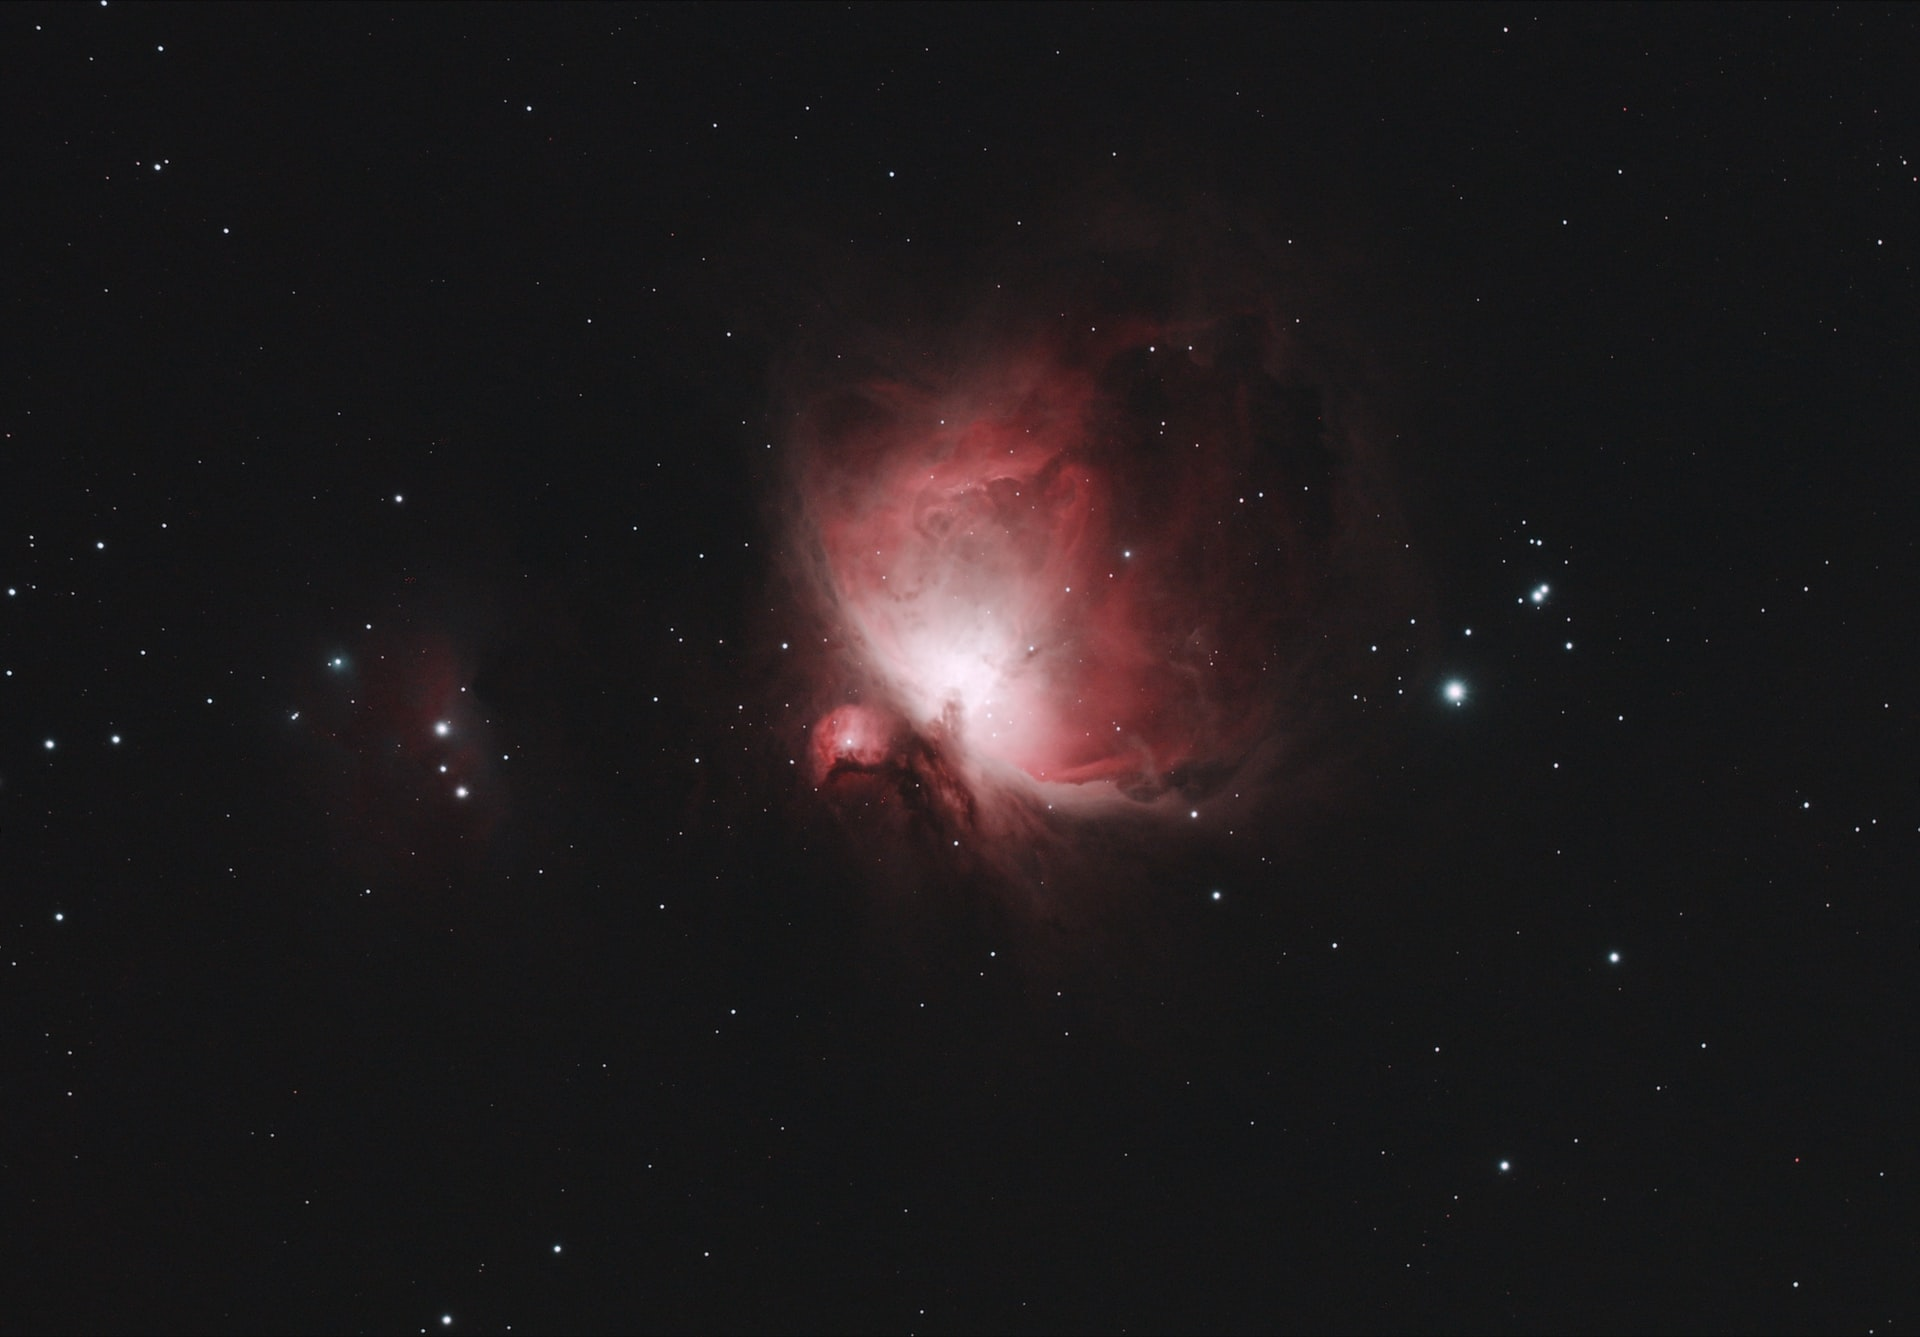
\includegraphics[width=\paperwidth]{./img/orion-nebula.jpg}}
\begin{frame}
    \titlepage
\end{frame}
}

\begin{frame}
    %\frametitle{Outline}
    \tableofcontents
\end{frame}

\begin{frame}
    \frametitle{\texttt{man slides}}

    (Interactive) course on web security based on Carsten Eiler's book "You've Been Hacked".
    
    Who is the audience? How can I use the book? How can I explore the app?
\end{frame}

\begin{frame}
    \frametitle{\texttt{whoami}}
    short intro/bio.
\end{frame}

\section{0x0: Preliminaries}

{
%\usebackgroundtemplate{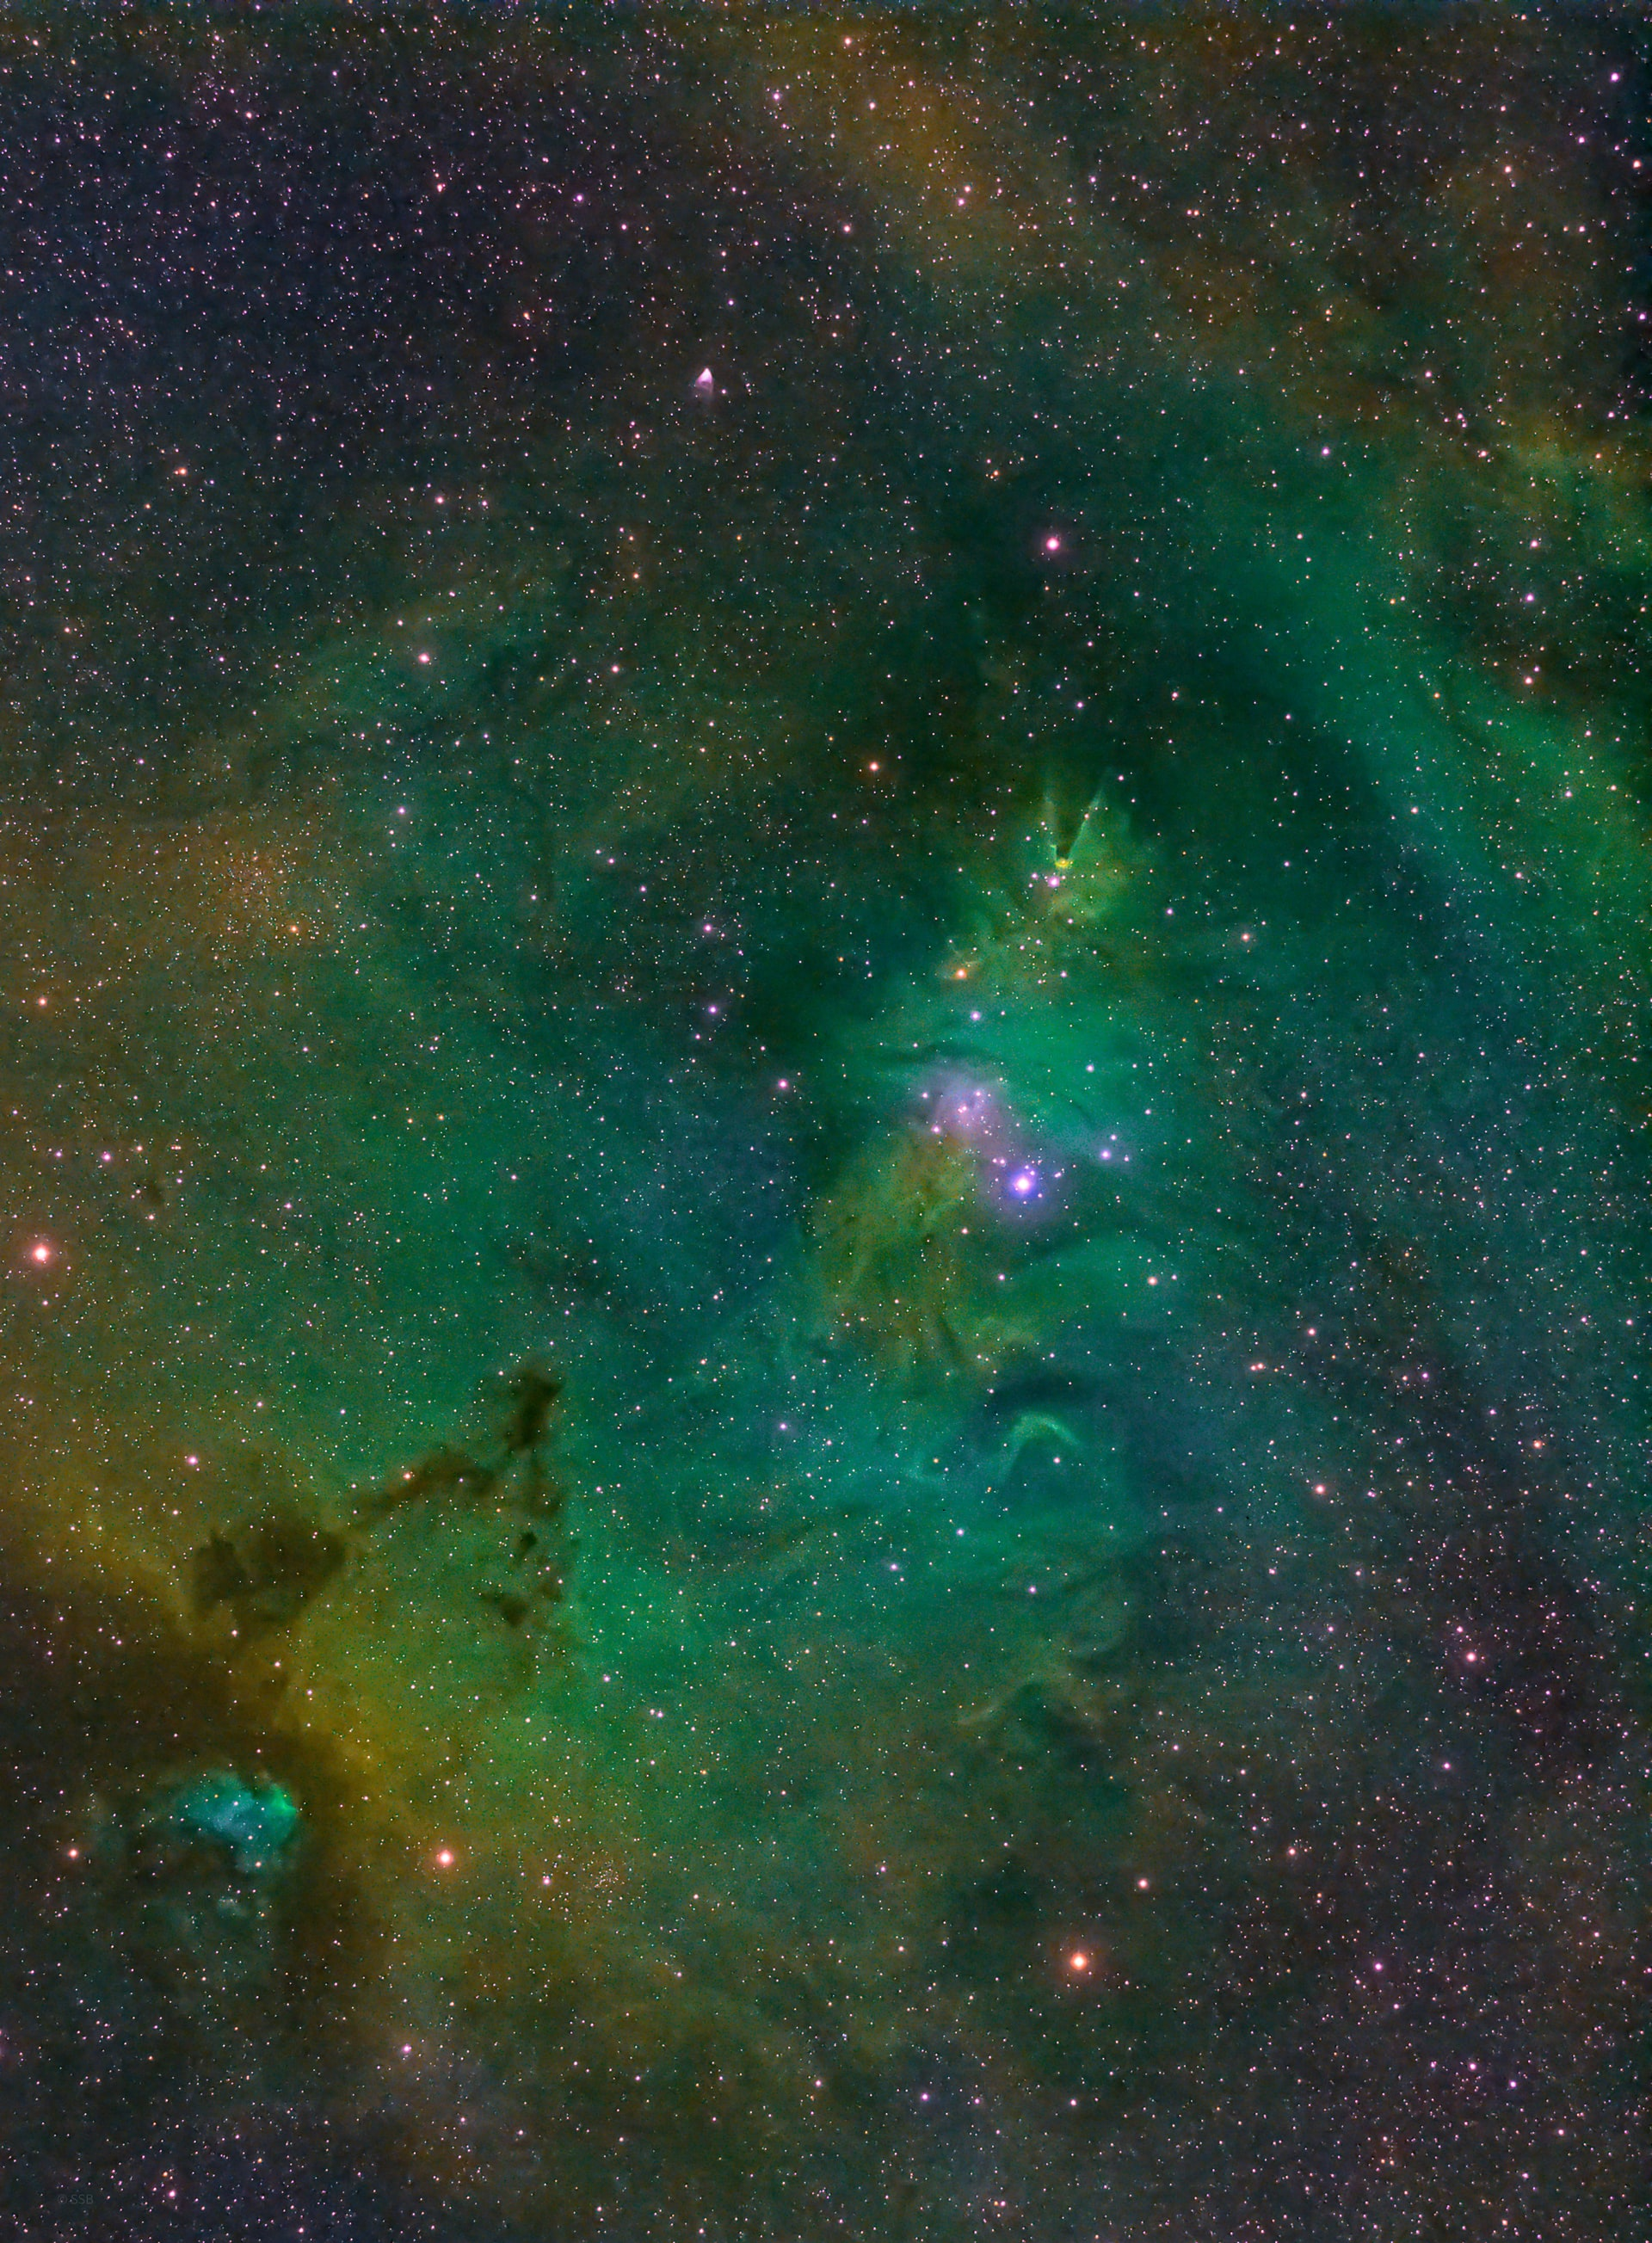
\includegraphics[width=\paperwidth]{./img/aldebaran.jpg}}
\begin{frame}
\huge{\textcolor{white}{\textbf{0x0: Preliminaries}}}
\end{frame}
}

%\begin{frame}
	\frametitle{Conventions}
	\begin{itemize}
		\item Alice, Bob: legitimate users
		\item Eve: malicious user, attacker
		\item Server: web server running a web application
		\item Client: web browser (or computer running the web browser)
	\end{itemize}
\end{frame}

\begin{frame}
	\frametitle{GitHub Repo}
	\begin{itemize}
		\item \url{https://github.com/duplys/youve-been-hacked}
		\item Dockerfile \& setup instructions
		\item Write-ups
		\item Code
	\end{itemize}
\end{frame}

\begin{frame}
	\frametitle{Build Docker Image}
	\begin{itemize}
		\item Running the demo web application in a Docker container is the easiest way to get started
		\item \texttt{Docker} dir contains \texttt{Dockerfile} for the vulnerable web application
		\item \texttt{Makefile} (\texttt{make build}) or \texttt{docker-compose}
	\end{itemize}
	
\end{frame}

\begin{frame}[fragile]
	\frametitle{Starting Docker Containers}
	\begin{itemize}
        \item You'll need an empty directory \texttt{tmp} in the \texttt{Docker} dir
		\item In \texttt{Docker} dir, run \verb|$ docker-compose up|
	\end{itemize}
\end{frame}

\begin{frame}[fragile]
	\frametitle{Accessing ZAProxy}
	\begin{itemize}
		\item In your web browser, hit \verb|http://127.0.0.1:8080/zap/|
        \item For documentation, see \url{https://www.zaproxy.org/docs/docker/webswing/}
	\end{itemize}
\end{frame}

\begin{frame}[fragile]
	\frametitle{Accesing the vulnerable Web application}
	\begin{itemize}
		\item \verb|$ docker container inspect docker_vulnapp_1 | grep "IPAddress"|
	\end{itemize}
\end{frame}

\begin{frame}[fragile]
	\frametitle{Cleaning Up}
	\begin{itemize}
		\item Run \verb|$ docker-compose down|
	\end{itemize}
\end{frame}


% Next, go your web browser and visit `http://127.0.0.1:8080/zap/` (as [described here](https://www.zaproxy.org/docs/docker/webswing/))

Next, you'll need the IP address of the Docker container running the vulnerable application. To extract this, do:

```shell
$ % docker container inspect exciting_maxwell
[
	{
		"Id": "9ea057ec1cea78eb1ab3abe4ba9f1cadb42ab751bf7bc1c9b0f277a286eeeddf",
		"Created": "2020-11-20T19:35:08.9811261Z",
		
		-- snip --
		
		"Networks": {
			"hack-network": {
				"IPAMConfig": null,
				"Links": null,
				"Aliases": [
					"9ea057ec1cea"
				],
				"NetworkID": "84aadd9f11e09968530e5093bdb8c95df7f30aa7efa7526ab315e30558126e03",
				"EndpointID": "adc8e373fe433540b208498a592d3598d79cb46ab860d1a302301ae9378136b2",
				"Gateway": "172.19.0.1",
				"IPAddress": "172.19.0.2",
				"IPPrefixLen": 16,
				"IPv6Gateway": "",
				
				-- snip --
				```
				
				You'll need to import the dynamic SSL certificate into Firefox. (go to ZAP --> Option -> Dynamic SSL Certificates and download one...). 
				
				Now, in your Firefox browser you need to enter the following URL: `http://host.docker.internal:8888/daten/kapitel1.html`. The reason for this is that if you use `127.0.0.1` together with the ZAP proxy, once that HTTP request arrives at the proxy, the proxy running in a docker container tries to resolve it and hits itself. So you get a "connection refused" warning and a Bad Gateway HTML response.







\section{0x1: Web Security 101}

{
\usebackgroundtemplate{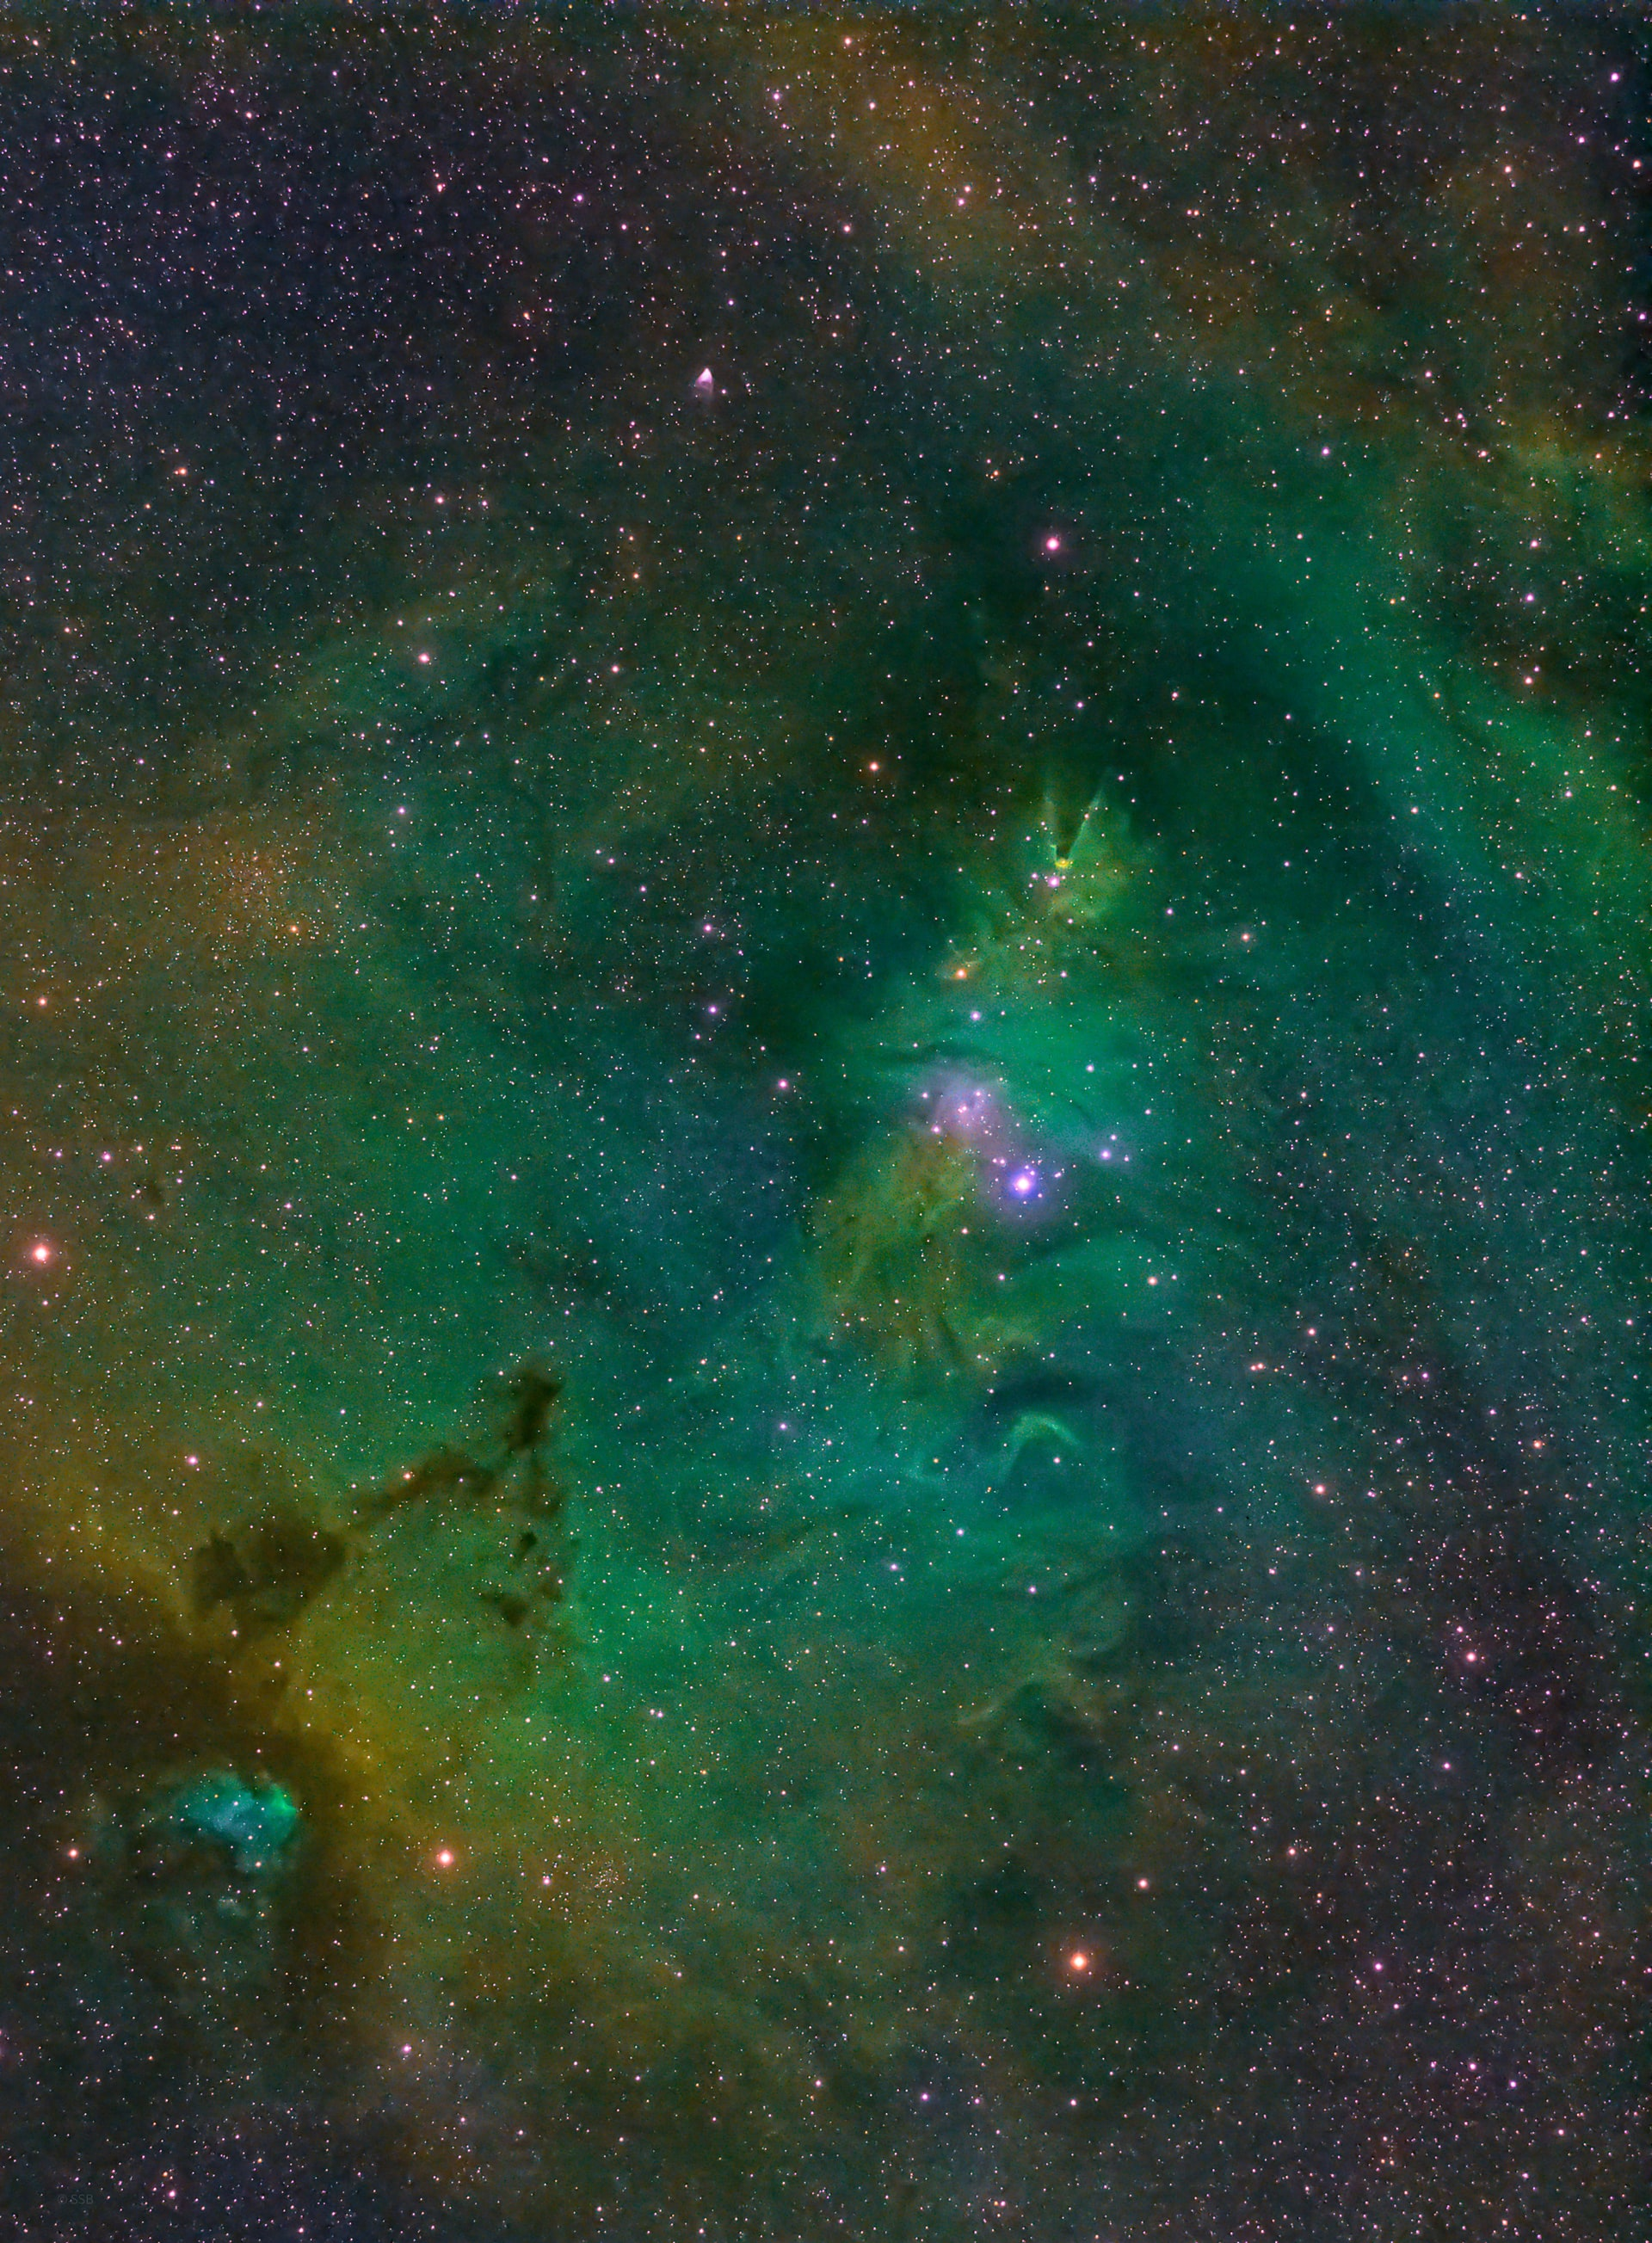
\includegraphics[width=\paperwidth]{./img/aldebaran.jpg}}
\begin{frame}
\huge{\textcolor{white}{\textbf{0x1: Web Security 101}}}
\end{frame}
}

\begin{frame}
    %\frametitle{How Do You Find Vulnerabilities in Web Applications?}
    In a nutshell, \textbf{to find vulnerabilities in your web application}, ...
    \begin{enumerate}
        \item ... test various values for parameters used by the web application and see what happens (conceptually similar to fuzzing)
        \item ... check web application code for bugs that may lead to security vulnerabilities (typically missing checks of input values or missing countermeasures against certain types of attacks)
    \end{enumerate}
\end{frame}

\begin{frame}
    %\frametitle{OWASP TOP 10}

    The \href{https://owasp.org/www-project-top-ten/}{Open Web Application Security Project (OWASP)} maintains a list of Top 10 vulnerabilities in web applications.

    \begin{center}
        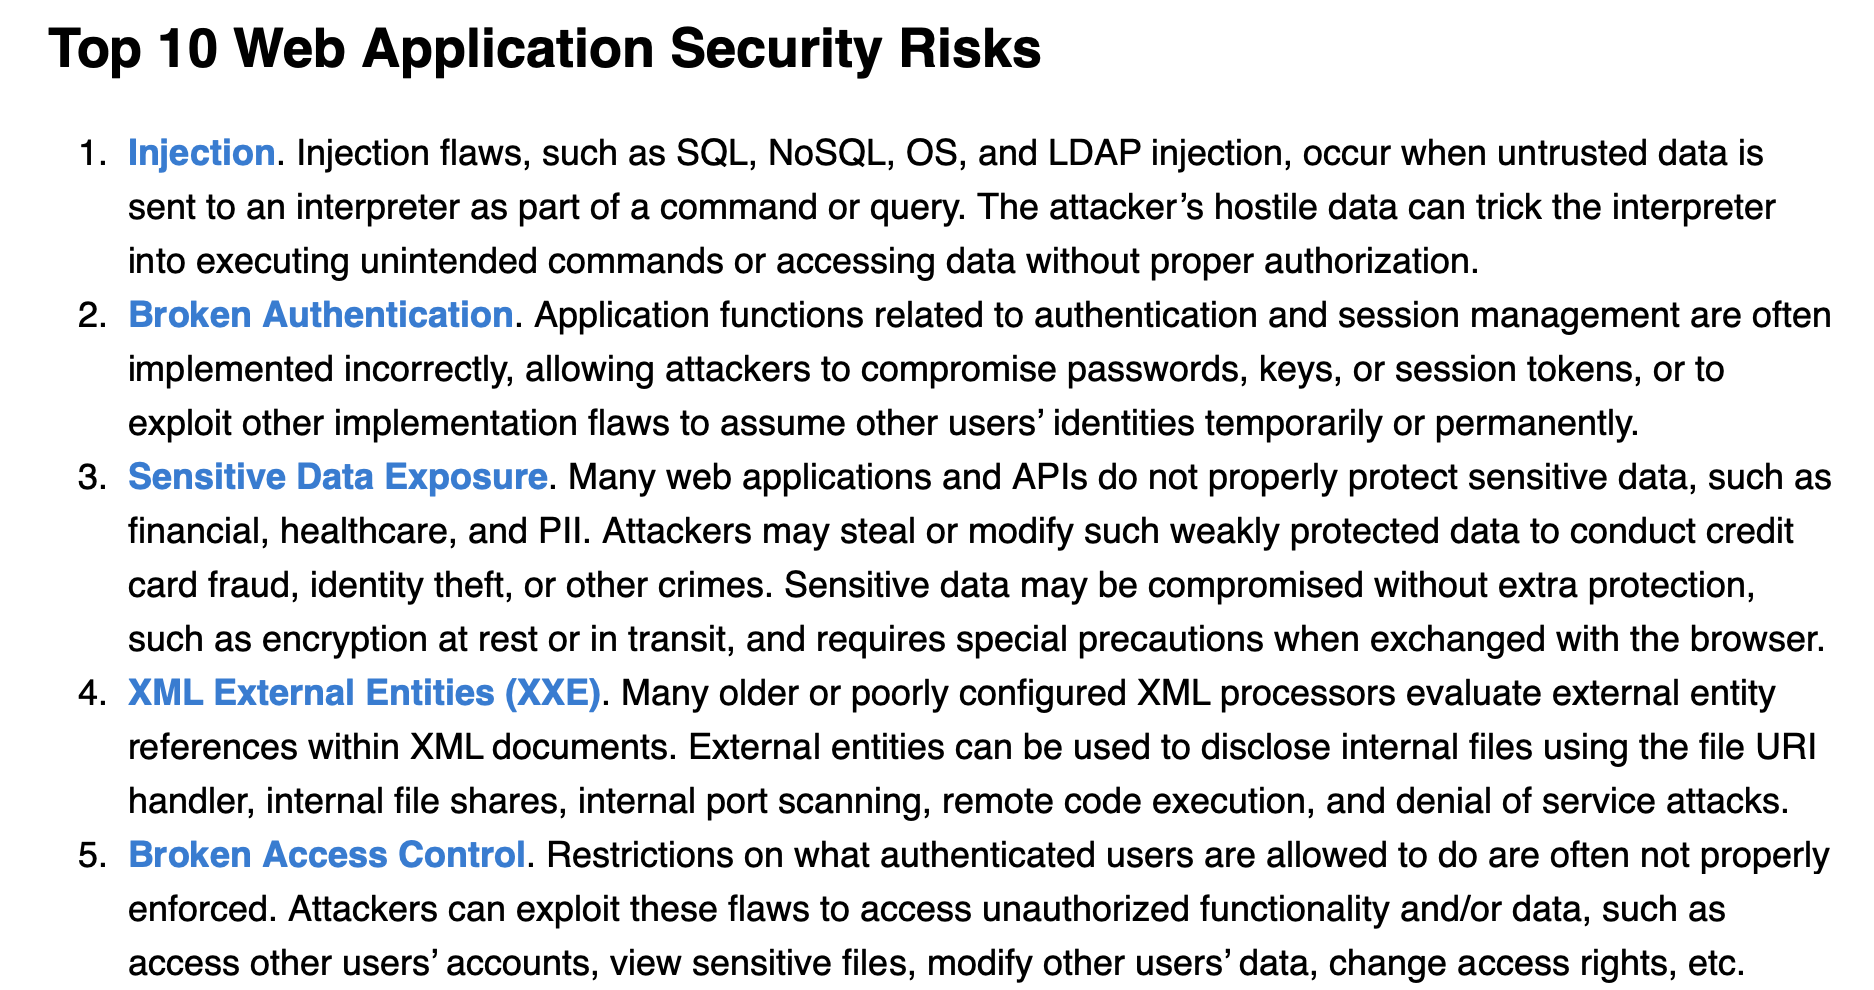
\includegraphics[scale=.35,angle=2]{img/owasp-top10.png}    
    \end{center}
\end{frame}

\begin{frame}
    \frametitle{Fahrplan}

    \begin{itemize}
        \item Get to know your target
        \item Test for attacks on web application's state
        \item Test for attacks on authentication
        \item Test for cross-site-scripting (XSS)
        \item Test for SQL injection
        \item Test for other injection-based vulnerabilities
        \item Test for attacks on file operations
        \item Test for buffer overflows, format strings and integer bugs
        \item Test for architectural attacks
        \item Test for attacks on the web server 
    \end{itemize}

\end{frame}

\section{0x2: Recon}

{
%\setbeamercolor{background canvas}{bg=yellow}
\usebackgroundtemplate{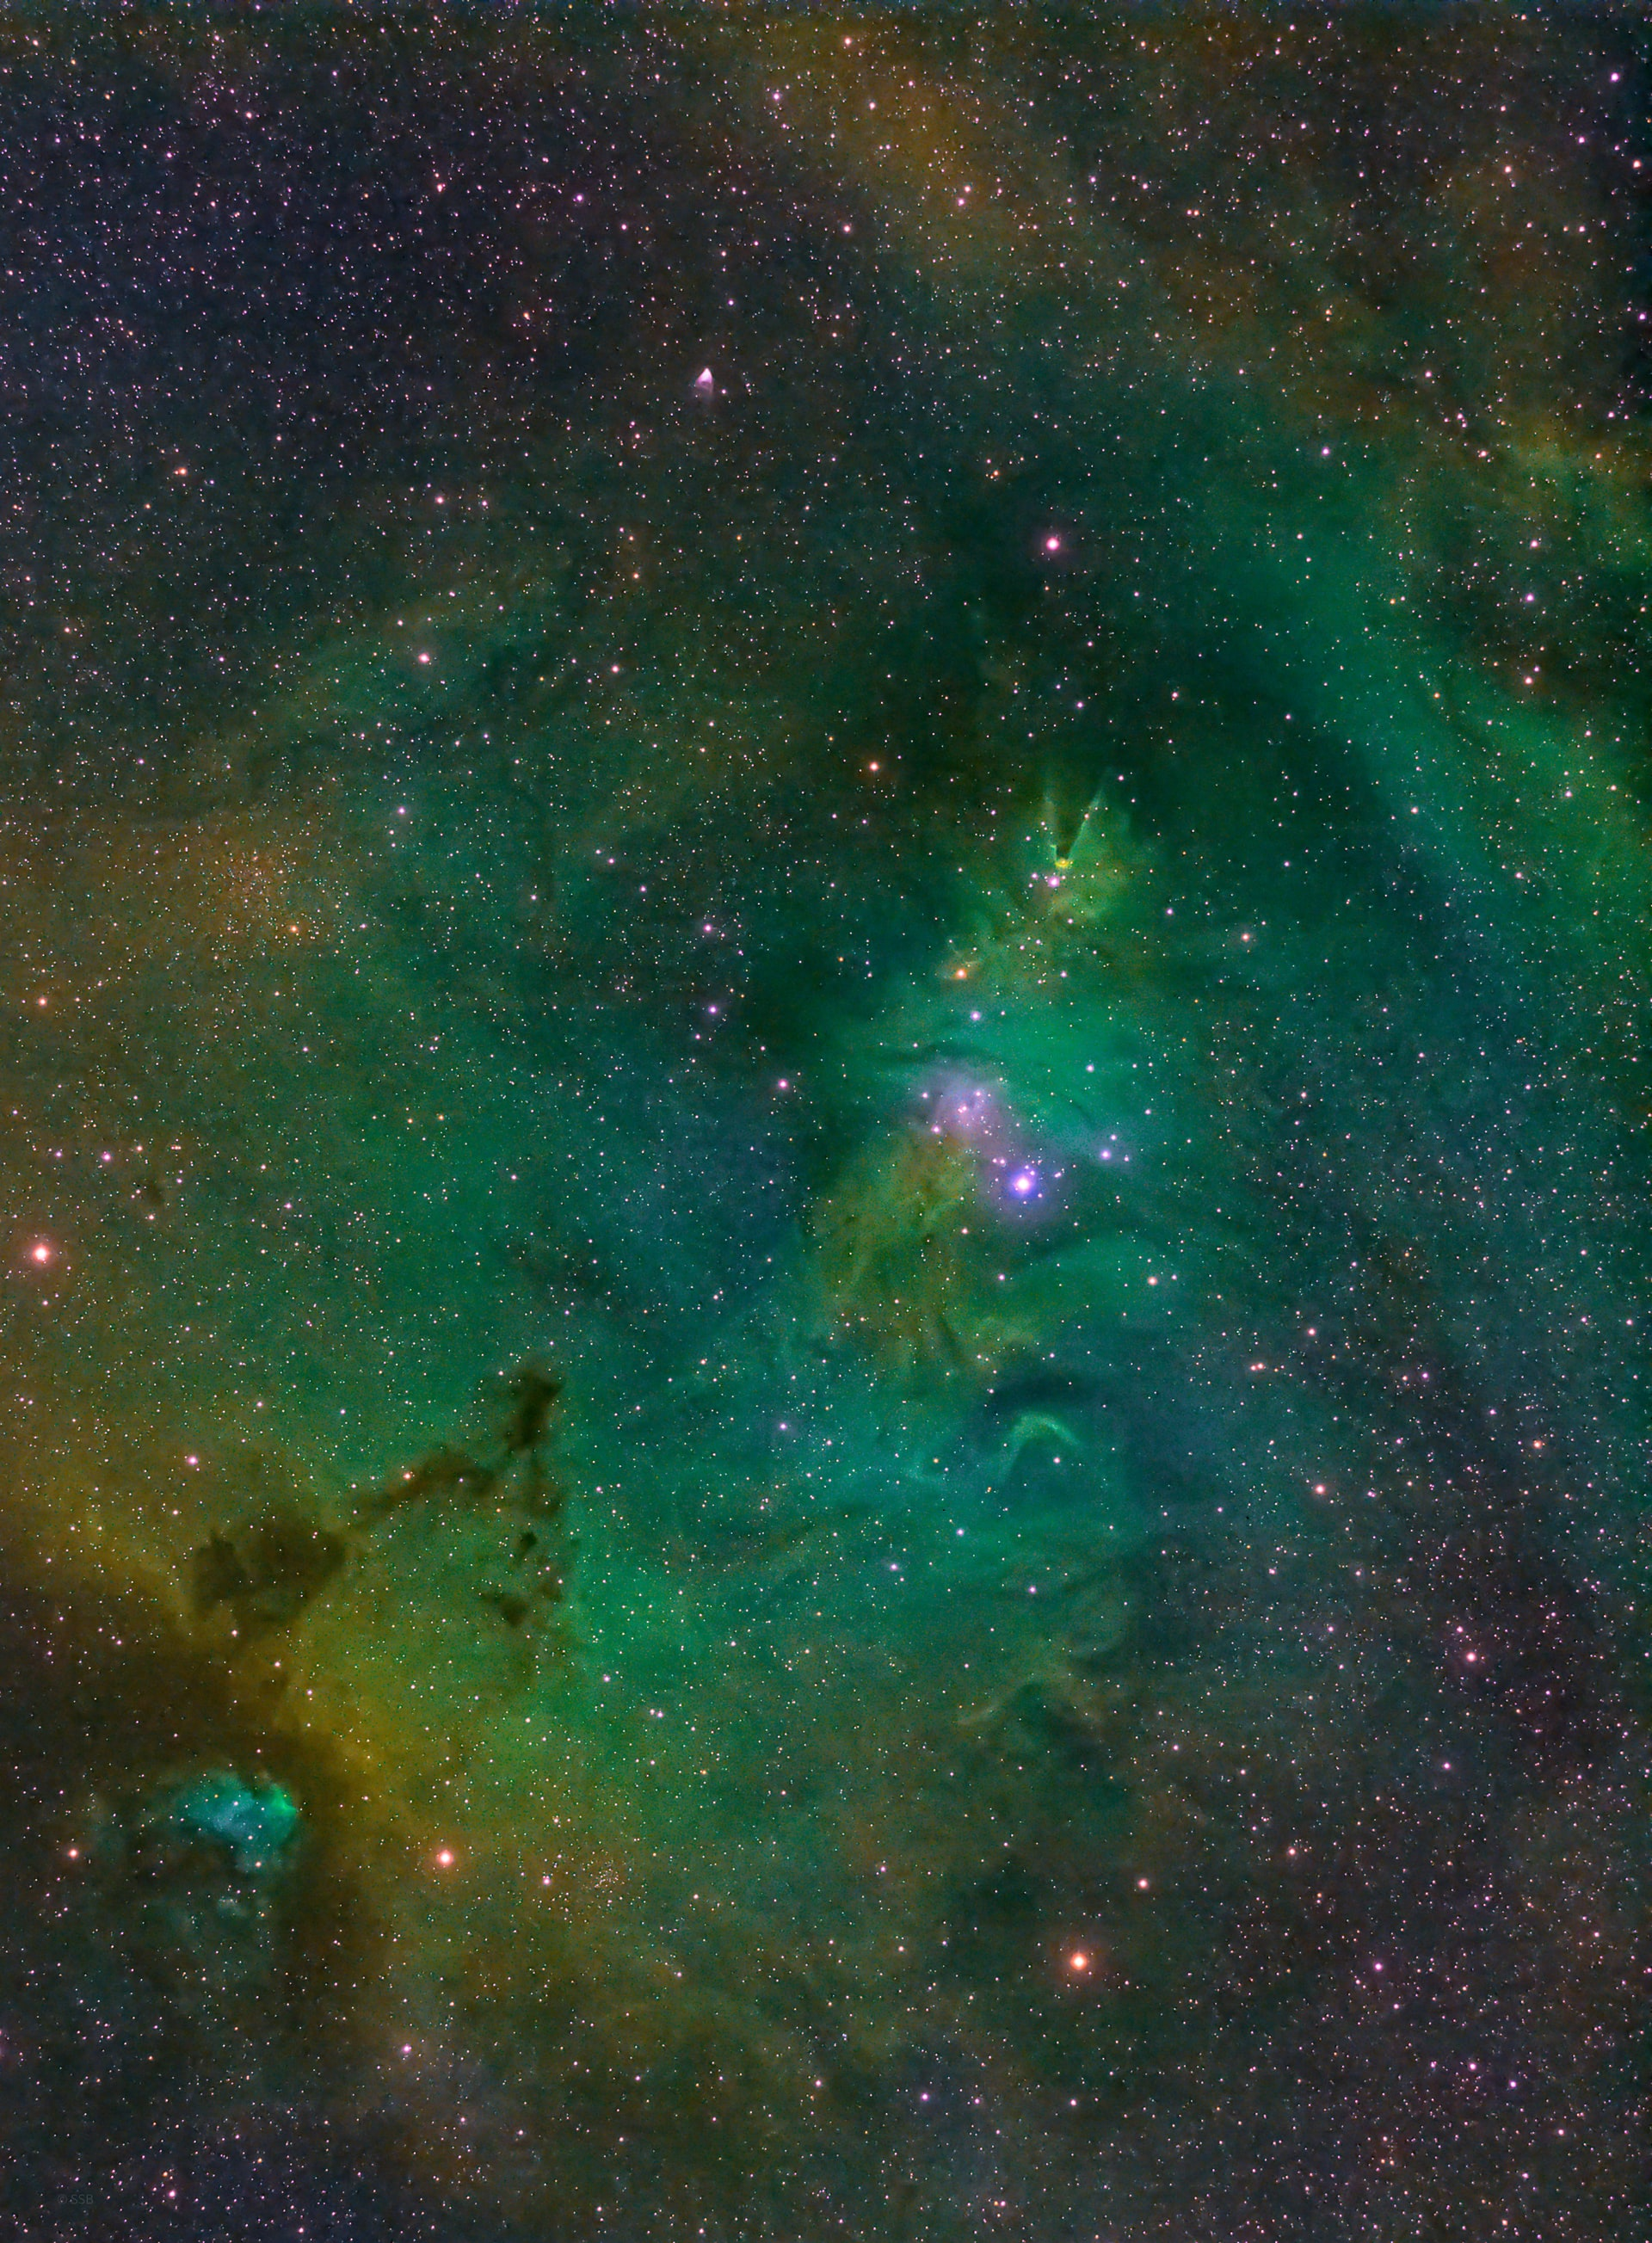
\includegraphics[width=\paperwidth]{./img/aldebaran.jpg}}
\begin{frame}
%\hspace{0.0cm}
\huge{\textcolor{white}{\textbf{0x2: Recon}}}
\end{frame}
}

%\usebackgroundtemplate{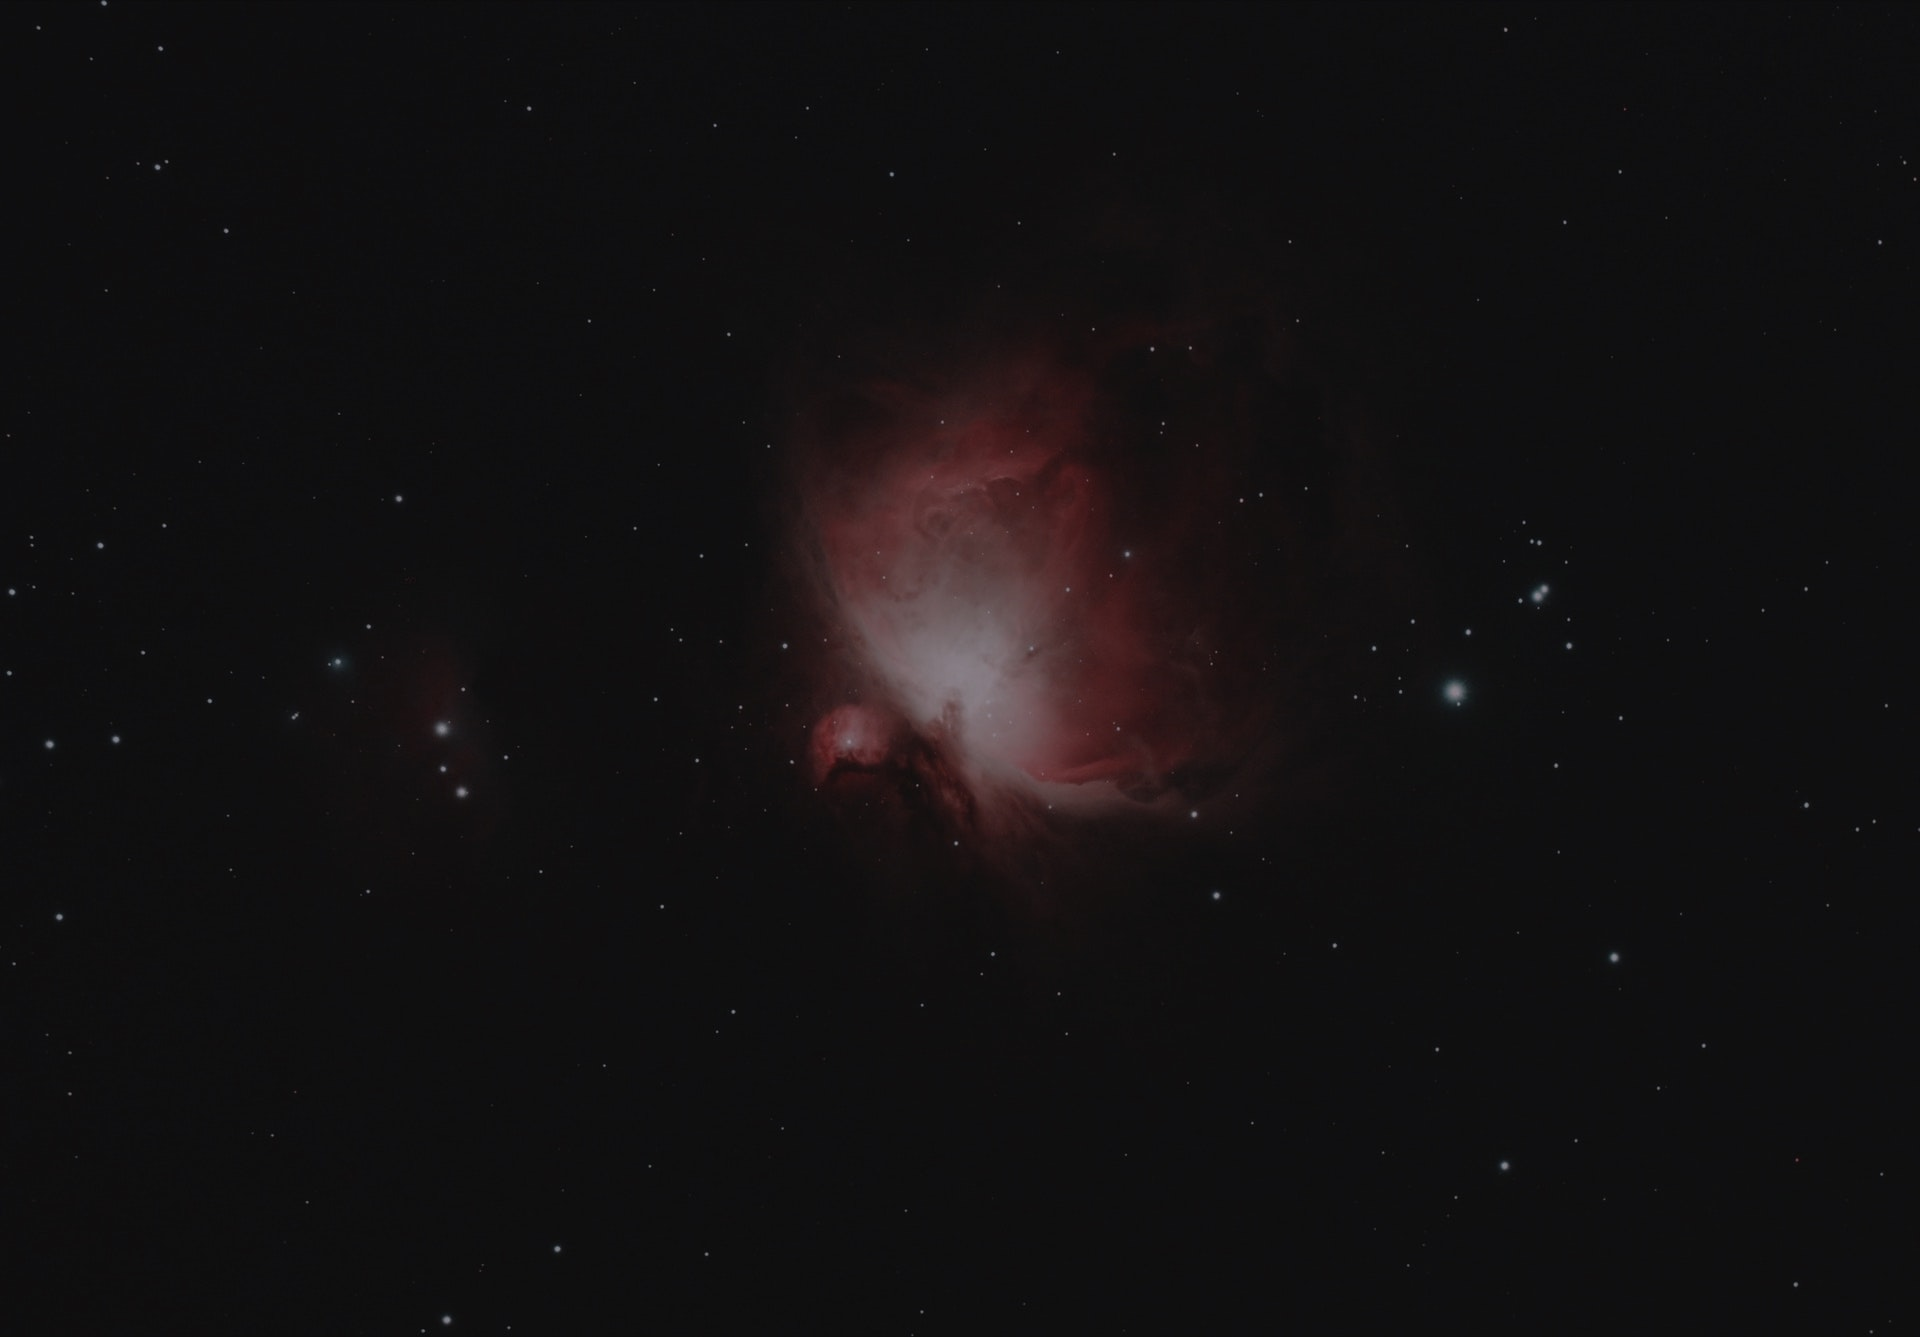
\includegraphics[width=\paperwidth]{./img/orion-nebula-copy.jpg}}

\begin{frame}%{Reconnaissance}
    \textbf{reconnaissance}: \textit{n}. 1. Military observation of a region to locate an enemy or ascertain strategic features. 2. Preliminary surveying or research.
\end{frame}

\begin{frame}
    \frametitle{Why Reconnaissance?}
    \begin{center}
        {\fontsize{70}{80}\selectfont \faQuestionCircle}
        \vfill
        Hint: consider the anatomy of a typical cybersecurity attack.
    \end{center}
\end{frame}

\begin{frame}
    \frametitle{Kill Chain}
    The term \href{https://en.wikipedia.org/wiki/Kill_chain}{kill chain} was originally coined by the military to describe the structure of an attack: finding adversary targets suitable for engagement; fixing their location; tracking and observing; targeting with a suitable weapon or asset to create desired effects; engaging the adversary; assessing the effects;
    \vfill
    In 2011, Hutchins et al~\cite{hutchins2011intelligence} from Lockheed-Martin expanded this concept to an \textbf{intrusion kill chain} for (network) security. They defined intrusion kill chain as reconnaissance, weaponization, delivery, exploitation, installation, command and control (C2), and actions on objectives. 
    \vfill
    Later on, security organizations have adopted this concept under the name "cyber kill chain".
\end{frame}

\begin{frame}
    \frametitle{Intrusion Kill Chain}
    \begin{figure}
        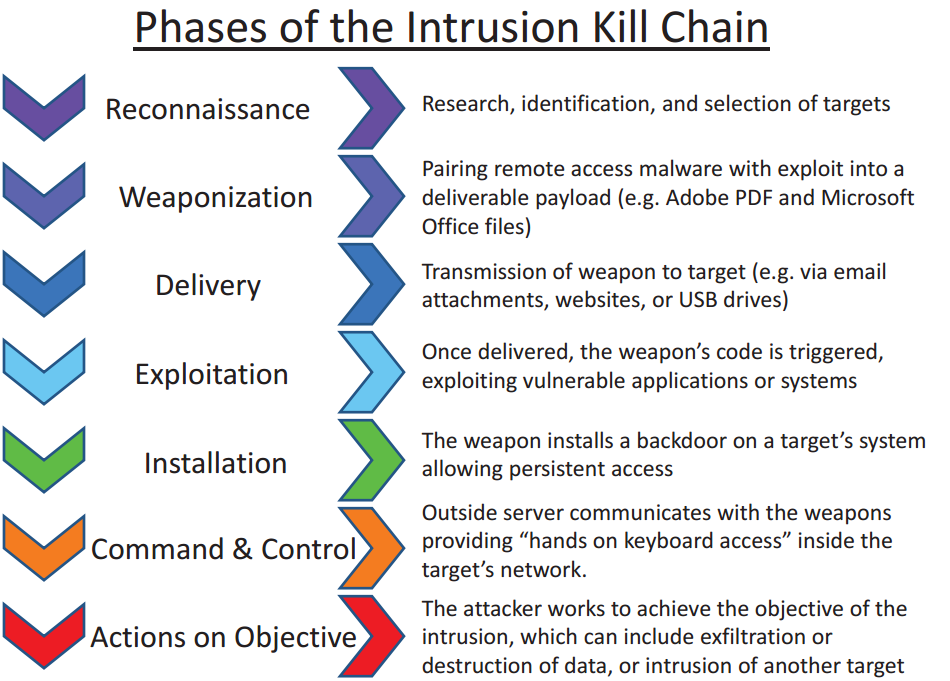
\includegraphics[scale=.35]{img/intrusion-kill-chain.png}
    \end{figure}
    \vfill
    \small{Source: \href{https://commons.wikimedia.org/wiki/File:Intrusion_Kill_Chain_-_v2.png}{Wikimedia Commons}.}
\end{frame}

\begin{frame}
    \frametitle{Mimicking the Attacker}
    Every attack starts by collecting information about the target, e.g., a web application ($\rightarrow$ cyber kill chain).
    \vfill
    Likewise, to test a web application for security vulnerabilities, you must first get to know it. You must understand what functions it uses and what parameters these functions have. You have to test every parameter whether it can be exploited (e.g., using illegitimate values). You need to check whether the web application code contains known vulnerabilities.
    \vfill
    \textbf{Systematic collection and documentation} allows you to understand what a real attacker would learn and where she could break your application's security.
\end{frame}

\begin{frame}
    \frametitle{Collecting Rudimentary Information}
    Document any \textbf{easy-to-spot hints} to security vulnerabilities:
    \begin{itemize}
        \item Suspicious comments in the HTML code (\texttt{<!-- default password:...})
        \item Sensitive information embedded in the HTML code
        \item Error messages from the web application
        \item Error messages from the web server and HTTP responses
    \end{itemize}
\end{frame}


\begin{frame}
    \frametitle{Learning the Web Application Structure}
    Catalogue \textbf{all pages, resources and parameters} that belong to or are used by the web application:
    \begin{itemize}
        \item using a general-purpose tool like \href{https://www.gnu.org/software/wget/}{\texttt{wget}}
        \item using a special-purpose tool like the \href{https://www.zaproxy.org/}{OWASP Zed Attack Proxy (ZAP)} crawler
        \item by manually visiting all web pages of the application (works well for small web applications)
    \end{itemize}
    \vfill
    While \texttt{GET} parameters are displayed in the URL, you'll need a web proxy like OWASP ZAP to access \texttt{POST} parameters and cookies.
    \vfill
    If your web application has different roles (guest, admin, \ldots), you'll have to test it for all these roles (i.e., first as a guest, then logged in as admin, etc.)
\end{frame}

\begin{frame}
    \frametitle{Investigating Individual Web Pages}
    Visit all pages and \textbf{inspect their source code}. Look for things like:
    \begin{itemize}
        \item \textbf{Leaky HTML comments} (comments containing e.g., code fragments, configuration parameters, server names, SQL table descriptions, etc.)
        \item \textbf{Hidden input fields} (\texttt{<input type='hidden' ...>})
        \item \textbf{SQL queries} printed in the page source due to programming or configuration errors (reveal the structure of the database and the queries used)
        \item \textbf{IP addresses of internal servers}
        \item \textbf{Web or email addresses}, e.g., email addresses of the developers (might reveal who wrote the application. Maybe it's just an optical tweak of a well-known application?)
    \end{itemize} 
    

\end{frame}

\begin{frame}
    \frametitle{Investigating Parameters}
    Investigate \textbf{all parameters} passed to the application:
    \begin{itemize}
        \item What happens when you change their values or use invalid values, e.g., a string instead of an integer?
        \item Do invalid parameters return error message that leak information about the application like database table names?
    \end{itemize}
\end{frame}

\begin{frame}
    \frametitle{Collecting More Information}
   \begin{itemize}
       \item Are there unlinked resources likes directories or files?
       \item E.g., if there are links to files financial-report18.pdf and financial-report19.pdf, is there an unpublished file financial-report20.pdf?
       \item Are there any hints to the structure of file names or sub directories?
       \item E.g., if the web application contains user profiles, is it possible to access an arbitrary profile using \texttt{user-[number].html} or \texttt{user.php?id=[number]}?
       \item Are there unlinked sub-directories like \texttt{test/} or \texttt{admin/}?
       \item Does the web server contain unused libraries or example application code that contains hints to known vulnerabilities or the internals of the web application? 
       \item What else is running on the server? SSH?
   \end{itemize}
\end{frame}

\begin{frame}
    \frametitle{Investigating Client-Side Code}
    %One of the main differences between classic static websites and client-side code: JavaScript is stateful $\rightarrow$ the order of the user interactions might change the outcome of running the JS code.
    \textbf{What input parameters are sanitized} in the client-side code (JavaScript or plain HTML)?
\end{frame}

\begin{frame}
    \frametitle{Investigating Client-Side Code: Static Pages}
    If user input is checked, i.e., sanitized, at client side (either in JavaScript or in HTML), chances are that no sanitization is implemented on the server. 
    
    Because an attacker can easily manipulate the client-side code, she can manipulate the user inputs sent to the server.
\end{frame}

\begin{frame}
    \frametitle{Investigating Client-Side Code: Static Pages}
    Check \textbf{all input fields} like text input, drop-down menus, radio buttons and select tags for \textbf{constraints for their values}. E.g., is there a maximum text length for a text field? Are numeric input values scoped? If yes, change these values and check how the web application is behaving.
\end{frame}

\begin{frame}
    \frametitle{Investigating Client-Side Code: Static Pages}
    There are 3 ways to change the client-side values:
    \begin{itemize}
        \item Parameters transmitted via \texttt{GET} requests can be manipulated directly in the URL
        \item Parameters transmitted via \texttt{POST} requests can be manipulated directly in a local copy of the website code
        \item On the fly, using a proxy like the \href{https://www.zaproxy.org/}{OWASP ZAP} or web developer tools in the web browser
    \end{itemize}
\end{frame}

\begin{frame}
    \frametitle{Investigating Client-Side Code: Static Pages}
    Hidden forms (\texttt{type="hidden"}) are sometimes used to store values used by the web application. A classic mistake is to store the price of the items in a web shop application (since you can easily manipulate them before sending them to the server).
\end{frame}

\begin{frame}
    \frametitle{A Trivial Example}
    Say there is a drop-down menu to select the number of items to be added to a shopping cart. The drop-down menu allows numbers in the range 0 to 100. What happens when you set this parameter to a negative value and transmit it to the server?
    
    Maybe there is no sanitization on the server side because only values greater or equal to zero can be selected from the drop-down menu? In this case, the final price is calculated by multiplying the price of the item with a negative number.
\end{frame}

\begin{frame}
    \frametitle{Collecting JavaScript-related Information}
    After checking HTML, next step is to check the JavaScript code.
    \vfill
    \begin{itemize}
        \item Is JavaScript used to validate input data? If so, maybe the check on the server side is omitted. 
        \item What files and scripts are being loaded? Any known vulnerabilities?
        \item Are there vulnerabilities in the JavaScript program logic itself? Any logic flaws that can be exploited?
    \end{itemize}   
\end{frame}


\begin{frame}
    \frametitle{Reconnaissance of the Demo Application}
    \begin{figure}
        \centering
        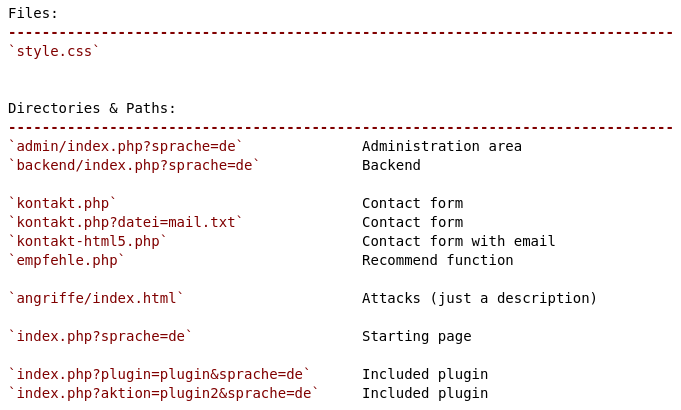
\includegraphics[scale=.4]{img/01-recon/recon-files-directories-paths.png}        
    \end{figure}
\end{frame}

\begin{frame}
    \frametitle{Reconnaissance of the Demo Application}
    \begin{figure}
        \centering
        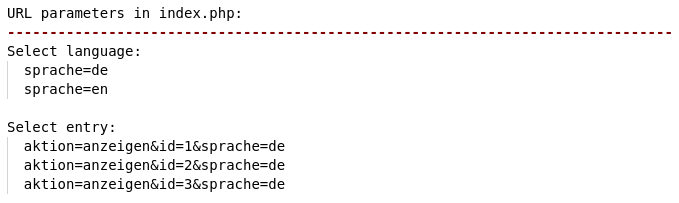
\includegraphics[scale=.4]{img/01-recon/recon-url-parameters.png}        
    \end{figure}
\end{frame}

\begin{frame}
    \frametitle{Reconnaissance of the Demo Application}
    \begin{figure}
        \centering
        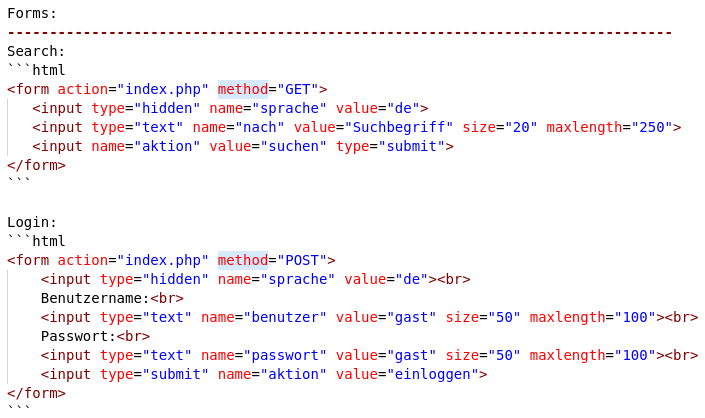
\includegraphics[scale=.4]{img/01-recon/recon-forms.png}        
    \end{figure}
\end{frame}

\begin{frame}
    \frametitle{Reconnaissance of the Demo Application}
    \begin{figure}
        \centering
        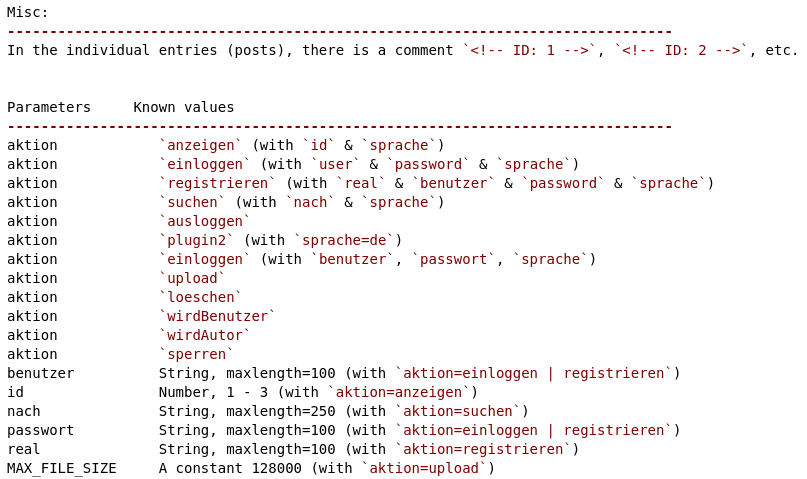
\includegraphics[scale=.4]{img/01-recon/recon-misc-and-parameters.png}        
    \end{figure}
\end{frame}

\begin{frame}
    \frametitle{Reconnaissance of the Demo Application}
    \begin{figure}
        \centering
        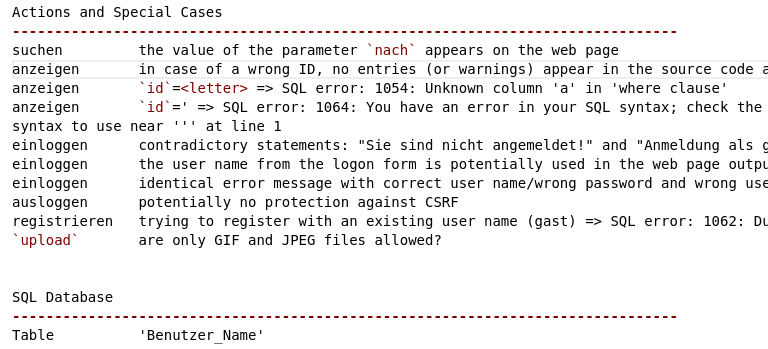
\includegraphics[scale=.4]{img/01-recon/recon-action-database.png}        
    \end{figure}
\end{frame}



%\begin{frame}
%    \frametitle{Sample frame title}
%    
%    In this slide, some important text will be
%    \alert{highlighted} because it's important.
%    Please, don't abuse it.
%    
%    \begin{block}{Remark}
%    Sample text
%    \end{block}
%    
%    \begin{alertblock}{Important theorem}
%    Sample text in red box
%    \end{alertblock}
%    
%    \begin{examples}
%    Sample text in green box. The title of the block is ``Examples".
%    \end{examples}
%
%\end{frame}

%\begin{frame}
%    \frametitle{Example}
%
%    \begin{itemize}
%        \item<1-> one
%        \item<2-> two
%        \item<3-> theorem
%    \end{itemize}
%
%\end{frame}

%\begin{frame}
%    \frametitle{Example 1}
%    One \pause
%    Two \pause
%    Three
%\end{frame}

\section{0x3: Attacks on Web Application's State}
{
\usebackgroundtemplate{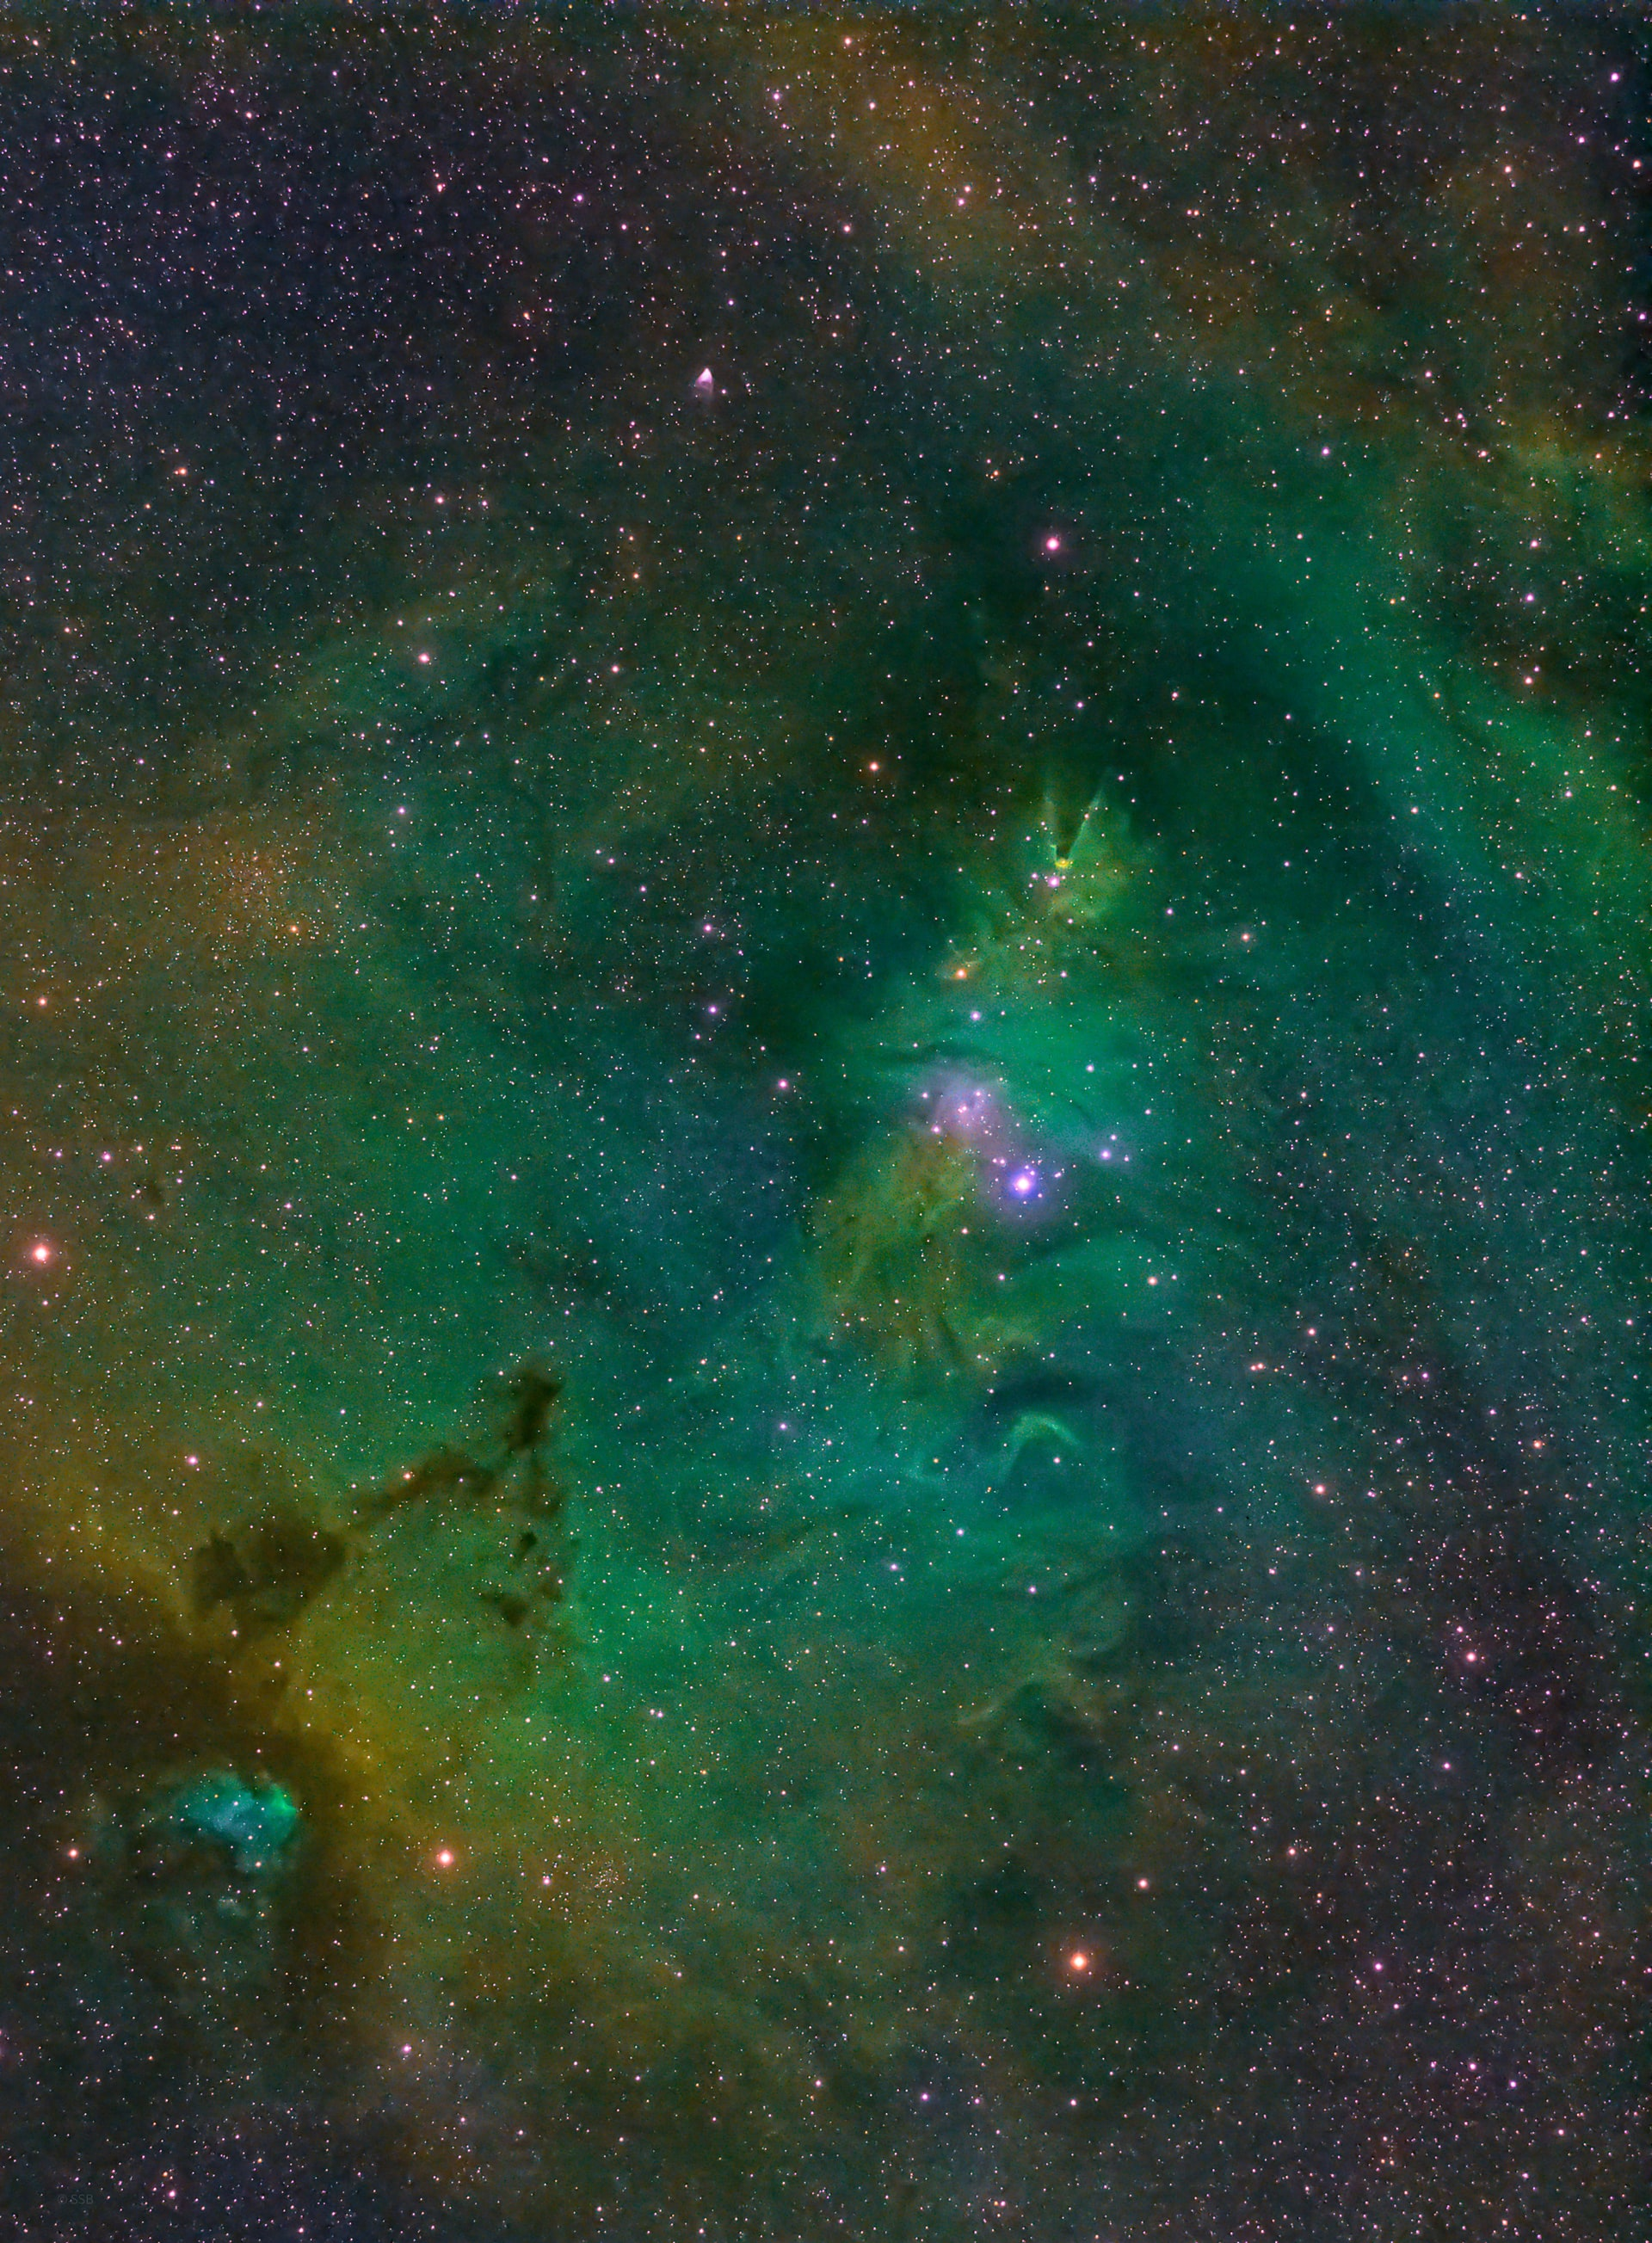
\includegraphics[width=\paperwidth]{./img/aldebaran.jpg}}
\begin{frame}
\huge{\textcolor{white}{\textbf{0x3: Stateful Attacks}}}
\end{frame}
}

%%%%%%%%%%%%%%%%%%%%%%%%%%%%%%%%%%%%%%%%%%%%%%%%%%%%%%%%%%%%%%%%%%%%%%%%%%%%%%%
%%% Attacks on Web Application State %%%%%%%%%%%%%%%%%%%%%%%%%%%%%%%%%%%%%%%%%%
%%%%%%%%%%%%%%%%%%%%%%%%%%%%%%%%%%%%%%%%%%%%%%%%%%%%%%%%%%%%%%%%%%%%%%%%%%%%%%%

\begin{frame}
    \frametitle{State in Web Applications}
        \begin{itemize}
        \item HTTP, the protocol for transferring data between the server and the client, is stateless
        \item Example: HTTP doesn't manage information about pages previously visited by the client, i.e., any URL can be requested by the client at any time. 
        \item If statefulness is required (e.g., page B shall only be served if the client has previously visited page A), the web application must manage a \textit{session}
    \end{itemize}
\end{frame}

\begin{frame}
    \frametitle{Statefulness: Web Shop Example}
    \begin{itemize}
        \item Malicious user adds items into the shopping cart
        \item She then skips the page where credit card information must be entered and proceeds directly to the checkout page
        \item If the web application doesn't enforce the correct sequence of pages, the user would successfully place an order without having entered any payment details 
    \end{itemize}
\end{frame}

\begin{frame}
    \frametitle{Managing State Information}
    There are two options to manage state information in web:
    \begin{itemize}
        \item the state information is stored on the server; the users are identified using a \textit{session ID}
        \item the state information is stored on the client
    \end{itemize}
\end{frame}

\begin{frame}[fragile]
    \frametitle{Hidden Input Fields}
    State information can be located in hidden input fields, e.g., 
    \begin{center}
        \begin{verbatim}
            <input name="id" value="1234" type="hidden">        
        \end{verbatim}
    \end{center}

    Such data fields can be easily manipulated using a tool like ZAP-Proxy or using web developer tools in the web browser. Thus, an attacker can easily manipulate hidden input fields. 
\end{frame}

\begin{frame}
    \frametitle{Detecting Hidden Input Field Vulnerabilities}
    For every hidden input field in the application, you must examine whether the web application's behavior changes if the values of these input fields are altered.

    A classical anti-pattern (luckily not so common anymore) is the use of hidden input fields for storing item price in a web shop. Yet another example is the storage of the user's status, e.g., a signed in user instead of a "guest" or administrator instead of a standard user.
\end{frame}

\begin{frame}
    \frametitle{Defending against Hidden Input Field Attacks}
    \begin{itemize}
        \item Core issue with hidden input fields: state information is stored \textit{on the client} where it can be easily manipulated by a malicious user
        \item Main defense philosophy: \textit{never trust the client}
        \item Critical information must always be stored on the server
        \item Values received from the client must always be checked \& validated
        \item If values must be stored on the client (e.g., session IDs), they should be encrypted or hashed
    \end{itemize}     
\end{frame}

\begin{frame}
    \frametitle{URL Parameters}
    \begin{itemize}
        \item (State) information can be transmitted in the URL
        \item In contrast to forms, transmitting information via URL parameters does not require clicking a submit button
    \end{itemize}
\end{frame}

\begin{frame}[fragile]
    \frametitle{URL Parameters: Finding Vulnerabilities}
    \begin{itemize}
        \item Using URL parameters to transmit information is a threat, because it is trivial to manipulate them
        \item Look for URL parameters identified during the recon phase
        \item Investigate what happens when you change these parameters. Does this cause an unexpected and unintended change of the state of the web application?
        \item \verb|http://www.webapp.example/editprofile.php?id=123|
        \item What happens when you change \verb|id|? Can you edit the profile of a different user?
        \item Are there (hidden) parameters to activate debug information, e.g., \verb|debug=on|, \verb|debug=1| or \verb|debug=true|?
    \end{itemize}
\end{frame}

\begin{frame}
    \frametitle{Defending against URL Parameter Manipulation}
    \begin{itemize}
        \item Core issue with URL parameters: state information is stored \textit{on the client} where it can be easily manipulated by a malicious user
        \item URL parameters must always be checked \& validated
        \item If possible, they should be encrypted or hashed
    \end{itemize}
\end{frame}

\begin{frame}
    \frametitle{Cookie Parameters}
    \begin{itemize}
        \item For a long time, cookies were the only option to persistently store data on the client
        \item It is still the prevailing solution
        \item Cookies are frequently used for user identification, e.g., at consecutive visits of a web application
        \item Attacks based on cookie manipulation are called \textit{cookie poisoning}  
    \end{itemize}
\end{frame}

\begin{frame}[fragile]
    \frametitle{Cookies}
    \begin{itemize}
        \item Persistent vs non-persistent cookies
        \item \verb|secure| vs \verb|HttpOnly| cookies
        \item Persistent cookies are stored on client's hard drive as long as their date is validated
        \item Non-persistent cookies are stored in RAM and are deleted when the web browser is closed
        \item \verb|secure| cookies are transmitted only via an HTTPS connection
        \item \verb|HttpOnly| cookies are transmitted via HTTP or HTTPS, but cannot be accessed by JavaScript
    \end{itemize}
\end{frame}

\begin{frame}
    \frametitle{Cookie Parameters: Storage and Manipulation}
    \begin{itemize}
        \item All web browsers store cookies in known file system locations and in known formats
        \item An attacker can easily manipulate this data before it is used by a web application
        \item It is possible to manipulate cookies \textit{on the fly}, e.g., using a tool like the ZAProxy
    \end{itemize}
\end{frame}

\begin{frame}
    \frametitle{Cookie Parameters: Storage and Manipulation}
    \begin{itemize}
        \item Unlike with URL parameters, the attacker can also manipulate the date when the cookie expires, i.e., she can manipulate the cookie's lifetime
        \item In general, cookies can give you access to things like sessions, profiles, etc.
    \end{itemize}
\end{frame}

\begin{frame}
    \frametitle{Cookie Parameters: Storage and Manipulation}
    Example:
    \begin{itemize}
        \item \texttt{weather.xyz} offers detailed weather information against payment
        \item \texttt{weather.xyz} uses cookies that contain \texttt{userID} to identify users
        \item The cookie is valid for the user's subscription period, e.g., a month
        \item Information stored in the cookie is processed by \texttt{weather.xyz} without additional authentication
        \item Attack 1: malicious user manipulates \texttt{userID} to access \texttt{weather.xyz} as another user
        \item Attack 2: malicious user extends their subscription by manipulating the cookie expiration date (by changing the Unix-timestamp in the cookie)
        \item Attack 3: cookies often store the number of failed login attempts. When they reach a specific threshold, say 5, \texttt{weather.xyz} deactivates that user account for 10 minutes to protect against brute force attacks. The attacker bypasses this defense by setting the value of failed login attempts to 0 after each login attempt. Since this can be easily automated, brute force attacks become trivial.
    \end{itemize}
\end{frame}

\begin{frame}
    \frametitle{Cookie Parameters: Finding Vulnerabilities}
    \begin{itemize}
        \item For every cookie found during recon phase, you must check whether a parameter manipulation results in an illegal state change of the web application
        \item Manipulation should also include cookie parameters like expiration
        \item To detect cookie-related vulnerabilities more efficiently, \textit{decrease} the expiration date and check whether the web application denies its service
        \item As an alternative -- if you have access to the server-side source code of the web application -- check whether the source code uses the cookie expiration date as input parameter
    \end{itemize}
\end{frame}

\begin{frame}
    \frametitle{Cookie Parameters: Defending Against Attacks}
    \begin{itemize}
        \item In general, cookie poisoning -- attacks that manipulate cookies -- cannot be eliminated
        \item Cookies are stored on the client and a malicious user can always manipulate data on the client (even data of other users)
        \item Two prominent attacks in this context are \textit{cross-site-scripting} (XSS) and \textit{cross-site-request-forgery} (CSRF)
        \item Attacker exploits web browser capabilities to set a cookie for a different domain
    \end{itemize}
\end{frame}

\begin{frame}
    \frametitle{Cookie Parameters: Defending Against Attacks}
    \begin{itemize}
        \item As a general rule, never trust data supplied by the client
        \item For example, store subscription's expiration date or the number of failed login attempts on the server
        \item If storing data on the client is unavoidable, encrypt or hash that data
        \begin{itemize}
            \item Question to the audience: why?
        \end{itemize} 
    \end{itemize}
\end{frame}



%%%%%%%%%%%%%%%%%%%%%%%%%%%%%%%%%%%%%%%%%%%%%%%%%%%%%%%%%%%%%%%%%%%%%%%%%%%%%%%
%%% URL Jumping %%%%%%%%%%%%%%%%%%%%%%%%%%%%%%%%%%%%%%%%%%%%%%%%%%%%%%%%%%%%%%%
%%%%%%%%%%%%%%%%%%%%%%%%%%%%%%%%%%%%%%%%%%%%%%%%%%%%%%%%%%%%%%%%%%%%%%%%%%%%%%%

\begin{frame}
    \frametitle{URL Jumping}
    \begin{itemize}
        \item Eve abuses the intended sequence of web pages. This gives her access to functions that by design must be unavailable at that point in time. 
    \end{itemize}
\end{frame}

\begin{frame}[fragile]
    \frametitle{URL Jumping: An Example}
    In a typical web shop, the intended sequence of transactions -- i.e., pages that a shop's customer visits -- could look something like this:
    \begin{enumerate}
        \item Search for a suitable product at \exurl{catalogue.php}
        \item add an article to the shopping cart at \exurl{add.php}
        \item verify the customer order at \exurl{order.php}
        \item provide shipping information (customer's postal address) at \exurl{shipping.php}
        \item enter credit card information at \exurl{payment.php}
        \item checkout \& finish the order at \exurl{checkout.php}
    \end{enumerate}
\end{frame}

\begin{frame}
    \frametitle{URL Jumping: An Example}
    \begin{itemize}
        \item If \attacker can jump from step 4 (\exurl{shipping.php}) directly to step 6 (\exurl{checkout.php}), she might be able to order an item without paying for it
        \item Another example: \attacker could try to post a message to an online forum with creating an account
        \item In general, \attacker tries to identify URLs that must be called in a specific sequence and tries to manipulate this sequence 
    \end{itemize}
\end{frame}

\begin{frame}
    \frametitle{URL Jumping: Locating the Vulnerabilities}
    \begin{itemize}
        \item Make a complete list of URLs in your web application and whether certain URLs must be called in a specific order
        \item Use information gathered during recon phase
        \item For every URL sequence:
        \begin{itemize}
            \item Call the URLs in the intended order and document the parameters passed to the web application
            \item Diverge from the intended sequence and see what happens. Are there any error messages (e.g., "You first must create a user") or are specific URL/pages not accessible?
            \item If there is no error message and the URLs can be accessed in any order, check whether this represents an actual, exploitable vulnerability
        \end{itemize}
    \end{itemize}
\end{frame}

\begin{frame}
    \frametitle{Defense against URL Jumping}
    \begin{itemize}
        \item URL jumping is a security issue only when the sequence in which URLs are accessed is relevant for the web application
        \item In that case, you need to check that the correct sequence is used, e.g., \texttt{checkout.php} would check if the user previously visited \texttt{payment.php} which, in turn, would check if the user previously visited \texttt{shipping.php}  
    \end{itemize}
\end{frame}

\begin{frame}
    \frametitle{Defending against URL Jumping}
    There are 3 options to identify a previously visited URL:
    \begin{enumerate}
        \item The URL (or the corresponding ID) is stored in a hidden input field or in an URL parameter
        \item The URL (or the corresponding ID) is stored in a cookie
        \item The URL, from which the user is allegedly coming, is compared to the \texttt{Referer} field value in the HTTP header 
    \end{enumerate}
\end{frame}

\begin{frame}[fragile]
    \frametitle{Defending against URL Jumping}
    \begin{itemize}
        \item As shown previously, option 1 (hidden input field) and option 2 (cookie) are insecure as they can be easily manipulate by \attacker
        \item That leaves us with option 3 (\texttt{Referer} value)
    \end{itemize}
    An HTTP request could look like this:
    \begin{center}
        \begin{verbatim}
            Get /checkout.php HTTP/1.1
            Host: www.shop.xyz
            User-Agent: Mozilla/5.0 (Macintosh; U; PPC Mac OS X; de-de) [...]
            Accept: */*
            Accept-Encoding: gzip, deflate
            Accept-Language: de-de
            Connection: keep-alive
            Referer: https://www.shop.xyz/payment.php
        \end{verbatim}
    \end{center}
\end{frame}

\begin{frame}
    \frametitle{Defending against URL Jumping}
    \begin{itemize}
        \item The \texttt{Referer} value is automatically set by the web browser
        \item In case of a bookmark or a direct entry in the web browser's address field the \texttt{Referer} value does not exist in the HTTP header
        \item However, the \texttt{Referer} value can be omitted by the web browser (for privacy reasons), removed from the HTTP request by a proxy or manipulated by \attacker
        \item \texttt{Referer} value can be manipulated using a tool like ZAProxy or using a dedicated client where the individual values of the HTTP header can be defined manually
        \item So \texttt{Referer} value is also insecure
    \end{itemize}
\end{frame}

\begin{frame}
    \frametitle{Defending against URL Jumping}
    \begin{itemize}
        \item In the end, the only effective defense against URL jumping -- similar to other attacks -- is to store state information on the server
        \item Specifically, the information about the visited URLs for each user can be stored temporarily in the web application (or persistently in a database)
    \end{itemize}
\end{frame}



%%%%%%%%%%%%%%%%%%%%%%%%%%%%%%%%%%%%%%%%%%%%%%%%%%%%%%%%%%%%%%%%%%%%%%%%%%%%%%%
%%% Session Hijacking %%%%%%%%%%%%%%%%%%%%%%%%%%%%%%%%%%%%%%%%%%%%%%%%%%%%%%%%%
%%%%%%%%%%%%%%%%%%%%%%%%%%%%%%%%%%%%%%%%%%%%%%%%%%%%%%%%%%%%%%%%%%%%%%%%%%%%%%%

\begin{frame}
    \frametitle{Session Highjacking}
    \begin{itemize}
        \item Numerous attacks can be alleviated by storing state information on the server (instead of client)
        \item In that case, the web application needs a way to identify the user
        \item The notion of a \emph{session} is used to associate state information (stored on the server) to a specific user
        \item The web application assigns each session a unique \emph{session identifier} (session-ID)
    \end{itemize}
\end{frame}

\begin{frame}
    \frametitle{Session Highjacking}
    \begin{itemize}
        \item Session-ID is a number or a combination of numbers and letters that uniquely identifies a session
        \item Session-ID is assigned to the client (user) upon the first HTTP request to the web application
        \item Every subsequent request carries the session-ID so that the web application can identify the client (user) and retrieve the corresponding state information stored on the server
    \end{itemize}
\end{frame}

\begin{frame}
    \frametitle{Session Highjacking}
    \begin{figure}[htb]
        \centering
        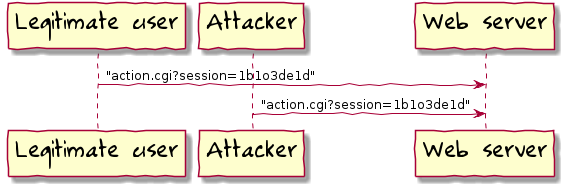
\includegraphics[scale=.5]{uml/session-hijacking.png}
    \end{figure}
    \begin{itemize}
        \item Because the session-ID must be stored on the client, it can be manipulated or stolen
        \item An attack exploiting this vulnerability is referred to as \emph{session hijacking}
        \item \Attacker gets hold of the session-ID information to gain unauthorized access to the web application
    \end{itemize}
\end{frame}

\begin{frame}[fragile]
    \frametitle{Session Highjacking}

    \begin{center}
        \begin{verbatim}
            Name=Alice
            userID=1234
            last=2021-08-24
        \end{verbatim}
    \end{center}

    \begin{itemize}
        \item A special case of session hijacking is the so-called \emph{authorization bypass}
        \item Example: web application identifies the client (user) based on a cookie containing the user name, the user ID and the date of the last session
        \item Is there are user with ID 1235?
        \item \Attacker can change \verb|userID| and use the manipulated cookie to take on the identity of another user
    \end{itemize}
\end{frame}

\begin{frame}
    \frametitle{Finding Session Highjacking Vulnerabilities}
    \begin{itemize}
        \item First, identify the session-ID in the web application, e.g., search for parameters whose names contain \texttt{ID}, \texttt{TOKEN}, \texttt{SESSIONID}, \texttt{ID} or similar strings. These parameters can be located in hidden input fields, URL parameters or in cookies.
        \item Once you identified a potential session-ID, change it and check whether you can impersonate another user
    \end{itemize}
\end{frame}

\begin{frame}
    \frametitle{Defending against Session Highjacking}
    \begin{itemize}
        \item Session hijacking requires a valid session-ID. \Attacker has essentially 4 options to get hold of it:
        \begin{itemize}
            \item Cross-site-scripting (XSS): XSS attacks are commonly used to steal cookies (more on this later). Make sure your web application has no XSS vulnerabilities. In addition, you can set \texttt{HTTPOnly} flag to prevent access to cookies from within JavaScript 
            \item Eavesdropping network traffic: if \attacker can read network traffic between the client and the web application, she can extract the session-ID. Ensure that you web application uses TLS (HTTPS).
            \item Searching logfiles: if \attacker has access to the web server (or proxy) logfiles, she can search them for session-IDs that were transmitted via \texttt{GET} requests. Session-ID should therefore be transmitted in cookies or via \texttt{POST} requests.  
            \item Brute-force attack: \attacker can try to guess the format of your session-IDs and try out various (random) combination until she finds a valid session-ID. You should use large random values as session-IDs.
        \end{itemize}
    \end{itemize}
\end{frame}

\begin{frame}
    \frametitle{Defending against Session Highjacking}
    \begin{itemize}
        \item Performing session identification based on the combination of the session-ID and the IP address of the client makes session hijacking more difficult
        \item Instead of the IP address, you can also use e.g., the \texttt{User-Agent} header (i.e., user the client browser "model" as an additional identification factor)
        \item To reduce session hijacking-related risks, you should end the sessions after a specific time and make the corresponding session-IDs invalid
        \item This can be done using a "hard" time-out (e.g., every session ends after 30 minutes) or a "soft" time-out (e.g., session ends after 10 minutes of inactivity)
    \end{itemize}
\end{frame}



%%%%%%%%%%%%%%%%%%%%%%%%%%%%%%%%%%%%%%%%%%%%%%%%%%%%%%%%%%%%%%%%%%%%%%%%%%%%%%%
%%% Session Fixation %%%%%%%%%%%%%%%%%%%%%%%%%%%%%%%%%%%%%%%%%%%%%%%%%%%%%%%%%%
%%%%%%%%%%%%%%%%%%%%%%%%%%%%%%%%%%%%%%%%%%%%%%%%%%%%%%%%%%%%%%%%%%%%%%%%%%%%%%%

\begin{frame}
    \frametitle{Session Fixation}
    \begin{figure}[htb]
        \centering
        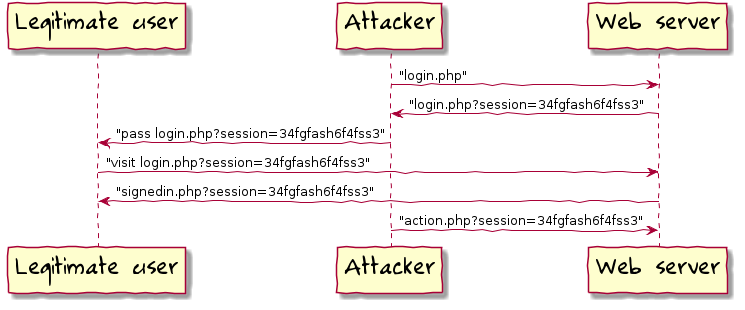
\includegraphics[scale=.5]{uml/session-fixation.png}
    \end{figure}
    \begin{itemize}
        \item Instead of stealing or guessing the session-ID, \attacker attempts to fixate other user's session-ID
        \item Session fixation attacks are typically web based and rely on session identifiers being accepted from URL parameters or POST data
        \item Example: \attacker sends Alice an email with a link to \texttt{login.php?session=34fgfash6f4fss3}
    \end{itemize}
\end{frame}

\begin{frame}
    \frametitle{Detecting Session Fixation Vulnerabilities}
    \begin{itemize}
        \item Use the information from the recon phase to identify session-IDs
        \item Call the web application with a session-ID that is already used, i.e., has been set by the web application
        \item Example: if the entry to the web application is \texttt{www.examle.xyz} and the web application, in turn, returns \texttt{www.example.xyz/index.php?session=[valid-session-ID]}, call this URL directly
        \item If you can login and your session-ID is \texttt{[valid-session-ID]}, you've found a session fixation vulnerability
        \item If session-ID is transmitted in a cookie, use ZAProxy to manipulate it   
    \end{itemize}
\end{frame}

\begin{frame}
    \frametitle{Defending against Session Fixation}
    \begin{itemize}
        \item Make sure your web application generates a new, random session-ID each time a user logs in
        \item The same behaviour must be implemented when a new users signs up
        \item Some web applications accept arbitrary session-IDs, i.e., session-IDs that they have not generated
        \item This makes Eve's life easier because she doesn't need to obtain a valid session-ID
        \item Thus, your web application should only accept session-IDs that it actually generated 
        \item Make sure it's impossible to reactivate expired sessions with known "old" session-IDs. If a session expired, a new session must be created with a new session-ID and a new state. Otherwise Eve can mount replay attacks.
        \item You should also leverage the information in HTTP header's \texttt{Referer} field. If the observed sequence of URLs doesn't match the expected sequence, either URL jumping is taking place or two clients (users) are using the same session-ID
    \end{itemize}
\end{frame}



%%%%%%%%%%%%%%%%%%%%%%%%%%%%%%%%%%%%%%%%%%%%%%%%%%%%%%%%%%%%%%%%%%%%%%%%%%%%%%%
%%% Clickjacking %%%%%%%%%%%%%%%%%%%%%%%%%%%%%%%%%%%%%%%%%%%%%%%%%%%%%%%%%%%%%%
%%%%%%%%%%%%%%%%%%%%%%%%%%%%%%%%%%%%%%%%%%%%%%%%%%%%%%%%%%%%%%%%%%%%%%%%%%%%%%%

\begin{frame}
    \frametitle{Clickjacking}
    \begin{figure}
        \centering
        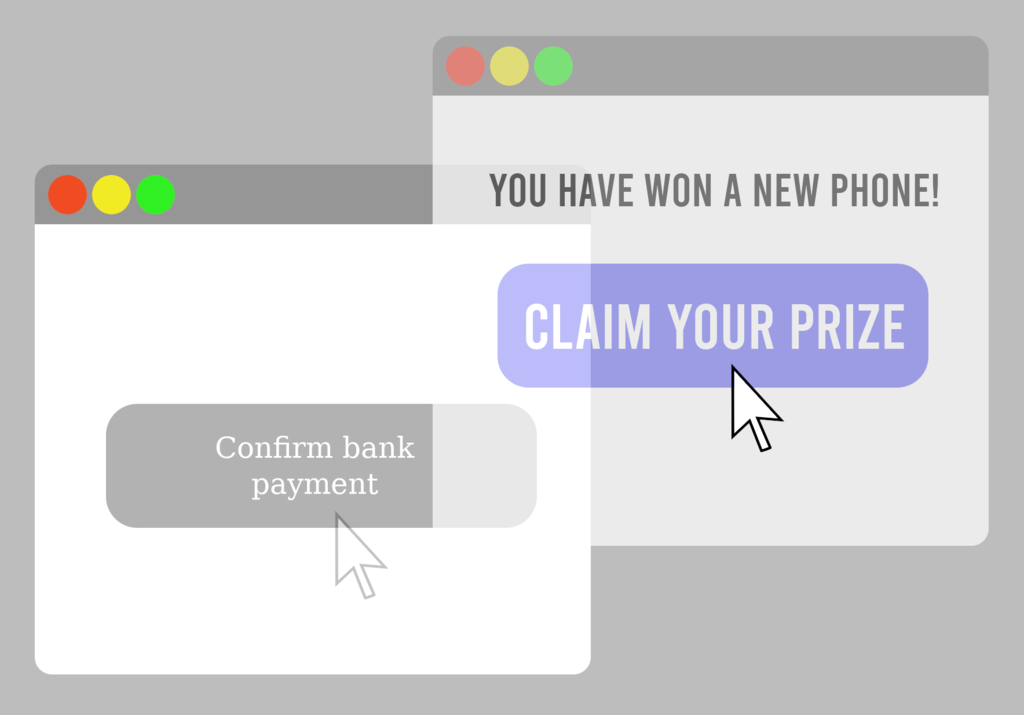
\includegraphics[scale=.3]{img/clickjacking.png}
    \end{figure}
    \begin{itemize}
        \item \eve tricks \alice into clicking on something different from what \alice perceives and, as a result, 
        \item This way, \eve can trick \alice into performing undesired actions by clicking on concealed links
        \item Clickjacking works because JavaScript allows to load a transparent layer over a web page and have the user's input affect that transparent layer without the user noticing
        \item For clickjacking to work, \alice must visit a page under Eve's control (because JavaScript is needed to create the transparent layer)
    \end{itemize}
    Image source: \href{https://upload.wikimedia.org/wikipedia/commons/thumb/0/0f/Clickjacking.png/1024px-Clickjacking.png}{Wikimedia}
\end{frame}

\begin{frame}
    \frametitle{Clickjacking}
    Example:
    \begin{itemize}
        \item Alice receives an email with a link to a video about a news item on a page under Eve's control
        \item Eve overlays a product page on Amazon on top of the "play" button of the news video
        \item Alice clicks on "play" to start the video, but actually buys the product from Amazon
        \item Eve can only send a single click, so she relies on the fact that Alice is both logged into Amazon.com and has the 1-click ordering enabled 
    \end{itemize}
\end{frame}

\begin{frame}
    \frametitle{Clickjacking}
    \begin{itemize}
        \item Technically, Eve embeds the target page an an iframe into the web page that will be displayed to Alice
        \item Eve reduces the size of the iframe such that only the target link is included; the rest of the target page is beyond the iframe
        \item Eve can configure the iframe to follow the mouse pointer. So regardless where Alice clicks, she will always clock on the target link
        \item Finally, Eve adjusts the opacity of the \texttt{div} element that spans the iframe such that the iframe becomes invisible to Alice
        \item After tricking Alice into clicking the target link, Eve can bring the visible page into the foreground so that Alice will likely not notice the attack
    \end{itemize}
\end{frame}

\begin{frame}
    \frametitle{Detecting Clickjacking Vulnerabilities}
    \begin{itemize}
        \item Check whether your application contains pages where only authenticated users can perform certain actions
        \item Then, check whether these pages can be embedded in iframes
    \end{itemize}
\end{frame}

\begin{frame}
    \frametitle{Defending against Clickjacking}
    \begin{itemize}
        \item To defeat clickjacking, you must prevent relevant web pages of your web application from being embedded in an iframe
        \item A \emph{framebuster} is a small JS script that prevents the web page from being displayed in a frame (however, HTML5 capabilities -- loading a page in a frame with the \texttt{sandbox} attribute -- allow Eve to bypass any framebusters)
        \item \texttt{X-Frame-Option} header can be used (by the web server) to specify preferred framing policy:
        \begin{itemize}
            \item \texttt{deny} prevents any framing
            \item \texttt{sameorigin} prevents framing by external sites
            \item \texttt{allow-from origin} allows framing only by the specified site
        \end{itemize}
        \item The \texttt{frame-ancestors} directive of the Content Security Policy can be used to allow or disallow embedding a web page in an iframe
    \end{itemize}
\end{frame}



%%%%%%%%%%%%%%%%%%%%%%%%%%%%%%%%%%%%%%%%%%%%%%%%%%%%%%%%%%%%%%%%%%%%%%%%%%%%%%%
%%% Cross-Site Request Forgery (CSRF) %%%%%%%%%%%%%%%%%%%%%%%%%%%%%%%%%%%%%%%%%
%%%%%%%%%%%%%%%%%%%%%%%%%%%%%%%%%%%%%%%%%%%%%%%%%%%%%%%%%%%%%%%%%%%%%%%%%%%%%%%

\begin{frame}
    \frametitle{Cross-Site Request Forgery}
    \begin{itemize}
        \item Cross-Site Request Forgery (CSRF) attacks exploit web application's trust in Alice to perform unauthorized actions on her behalf
        \item Eve's goal is to trick Alice into unknowingly submitting an HTTP/web request to a web application that Alice has privileged access to (but Eve does not)
        \item Unlike Cross-Site Scripting (XSS) which exploits the trust a user has for a particular site, CSRF exploits he trust that a site has in a user's browser
        \item 
    \end{itemize}
\end{frame}

\begin{frame}
    \frametitle{Cross-Site Request Forgery}
    \begin{itemize}
        \item At risk are web applications that perform actions based on input from trusted and authenticated users without requiring the user to authorize the specific action
        \item For instance, a user who is authenticated by a cookie saved in the user's web browser could unknowingly send an HTTP request to a site that trusts the user and thereby cause an unwanted action
    \end{itemize}
\end{frame}

\begin{frame}[fragile]
    \frametitle{Cross-Site Request Forgery}
    Example 1:
    \begin{itemize}
        \item \verb|www.server.xyz/app/index.php?action=logout| is used to log out users
        \item The web application identifies users through a session-ID stored in a cookie
        \item The cookie is automatically sent by the user's web browser
        \item The web application is an online forum where links can be stored in posts
        \item Eve publishes a post with the above link disguised by an \verb|<a href="...">more info here</a>|
        \item Alice clicks on the link and is logged out
    \end{itemize}
\end{frame}

\begin{frame}[fragile]
    \frametitle{Cross-Site Request Forgery}
    Example 2:
    \begin{itemize}
        \item New user is added when \verb|www.server.xyz/app/admin/adduser.php?name=NAME&pass=PWD| is called by an admin
        \item The web application identifies users through a session-ID stored in a cookie
        \item Eve prepares a malicious web page and tricks the admin to open this page
        \item The web page contains \verb|<img src=www.server.xyz/app/admin/adduser.php?name=eve&pass=eve">|
        \item The (loged in via cookie) admin opens the malicious page
        \item Admin's web browser sends a \verb|GET| request to load the image
        \item The URL to create a new user is called instead
        \item The cookie to authenticate the admin is automatically sent by her web browser
    \end{itemize}
\end{frame}

\begin{frame}[fragile]
    \frametitle{Cross-Site Request Forgery}
    Example 3:
    \begin{itemize}
        \item Instead of a \verb|GET| request, the web application uses a form -- and, thus, a \verb|POST| request -- to add new users:
        \begin{verbatim}
            <form method="post" action="http://www.server.xyz/app/admin/adduser.php">
              Name: <input name="username"> <br>
              Passwort: <input name="password"> <br>
              <input type=submit value="Add User">
            </form>
        \end{verbatim}
        \item The data sent to the application is in the \verb|POST| request, i.e., it doesn't show in the URL
        \item Eve prepares a malicious web page and tricks the admin to open this page
        \item The web page contains a form that is auto-submitted upon opening the pages:
        \begin{verbatim}
            <form name="csrf" method="post" action="http://www.server.xyz/app/admin/adduser.php">
              <input type="hidden" name="username" value="eve">
              <input type="hidden" name="password" value="eve">
            </form>
            <script>document.CSRF.submit()</script>
        \end{verbatim}
        \item The (loged in via cookie) admin opens the malicious page
        \item The form is submitted automatically, as if the admin clicked on "Add User"
        \item The cookie to authenticate the admin is automatically sent by her web browser
    \end{itemize}
\end{frame}

\begin{frame}[fragile]
    \frametitle{Cross-Site Request Forgery}
    Example 3 (cont'd):
    \begin{itemize}
        \item Eve prepares a malicious web page and tricks the admin to open this page
        \item The web page contains a form that is auto-submitted upon opening the pages:
        \begin{verbatim}
            <form name="csrf" method="post" action="http://www.server.xyz/app/admin/adduser.php">
              <input type="hidden" name="username" value="eve">
              <input type="hidden" name="password" value="eve">
            </form>
            <script>document.CSRF.submit()</script>
        \end{verbatim}
        \item The (loged in via cookie) admin opens the malicious page
        \item The form is submitted automatically, as if the admin clicked on "Add User"
        \item The cookie to authenticate the admin is automatically sent by her web browser
    \end{itemize}
\end{frame}

\begin{frame}
    \frametitle{Cross-Site Request Forgery}
    \begin{itemize}
        \item Essentially, it is sufficient to trick an authorized user to send a maliciously crafted HTTP request
        \item As a result, CSRF is not limited to web pages
        \item Any document format that supports scripting can be exploited, e.g., HTML e-mails and multimedia files
    \end{itemize}
\end{frame}

\begin{frame}
    \frametitle{Detecting CSRF Vulnerabilities}
    \begin{itemize}
        \item A web application is susceptible to CSRF when it implements actions that can be triggered via a static URL (\texttt{GET} request) or a static \texttt{POST} request (like a static form)
        \item To prevent CSRF attacks, the corresponding URLs or forms (\texttt{POST} requests) contain the so-called \emph{Anti-CSRF-Token}
        \item The \emph{anti-CSRF-token} is a random value that Eve cannot guess
        \item The action associated with the \texttt{GET} or \texttt{POST} request is only performed if the token contains the correct value
    \end{itemize}
\end{frame}

\begin{frame}
    \frametitle{Detecting CSRF Vulnerabilities}
    \begin{itemize}
        \item Thus, you need to check whether all \texttt{GET} and \texttt{POST} requests perform an action that requires authorization contain a CSRF-token  
        \item Check whether these requests contain parameters that change every time the request is Sensitive
        \item If any of these requests is static, i.e., doesn't change over time, the web application is vulnerable to CSRF
    \end{itemize}
\end{frame}

\begin{frame}
    \frametitle{Defending against CSRF}
    \begin{itemize}
        \item You must add a unique, random token to every relevant \texttt{GET} and \texttt{POST} request
        \item It is important that the token has sufficient entropy so that Eve cannot simply send multiple request with highly likely token values
        \item The web application must only perform actions when the correct token is supplied
        \item Then, Eve cannot prepare a valid request because she can't guess the random token value (she could learn the token value using XSS, though) 
        \item For really important actions, you should add an additional password check
    \end{itemize}
\end{frame}

\begin{frame}
    \frametitle{Defending against CSRF}
    \begin{itemize}
        \item 
    \end{itemize}
\end{frame}

\begin{frame}
    \frametitle{Defending against CSRF}
    \begin{itemize}
        \item 
    \end{itemize}
\end{frame}

\section{0x4: Attacks on Authentication}
{
\usebackgroundtemplate{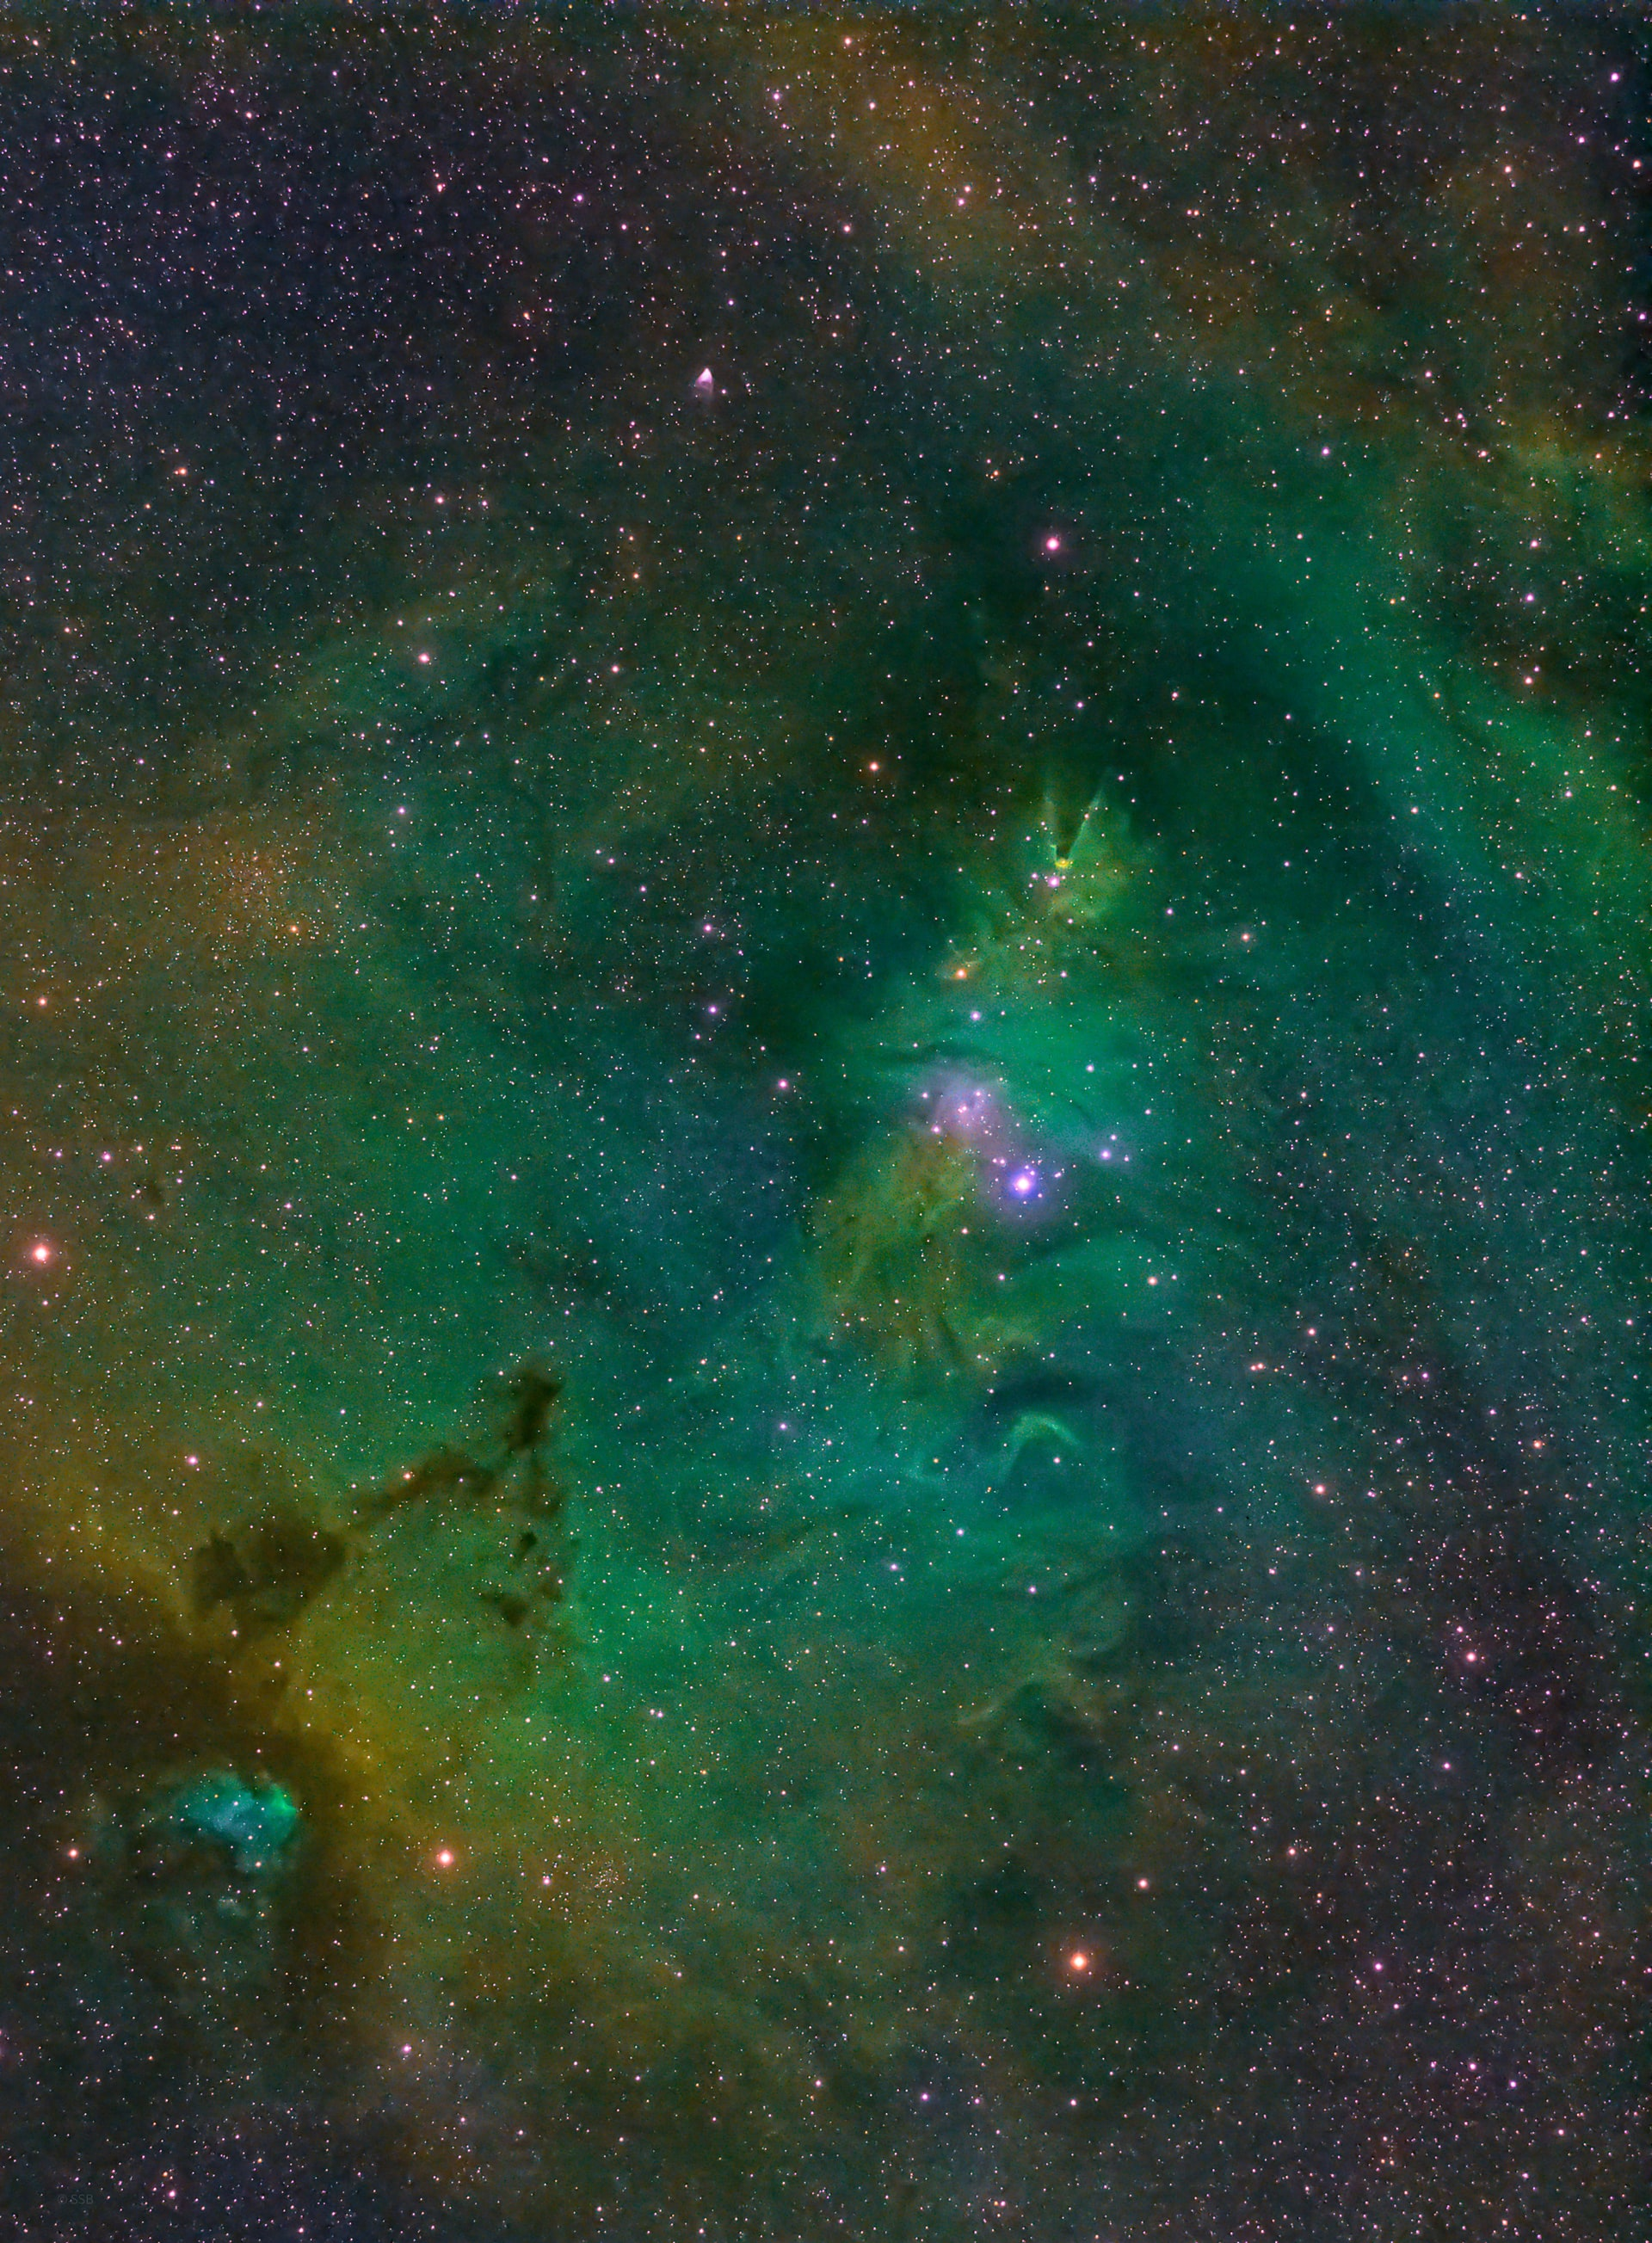
\includegraphics[width=\paperwidth]{./img/aldebaran.jpg}}
\begin{frame}
\huge{\textcolor{white}{\textbf{0x4: Attacks on Authentication}}}
\end{frame}
}

\section{0x5: Cross-Site-Scripting (XSS)}
{
\usebackgroundtemplate{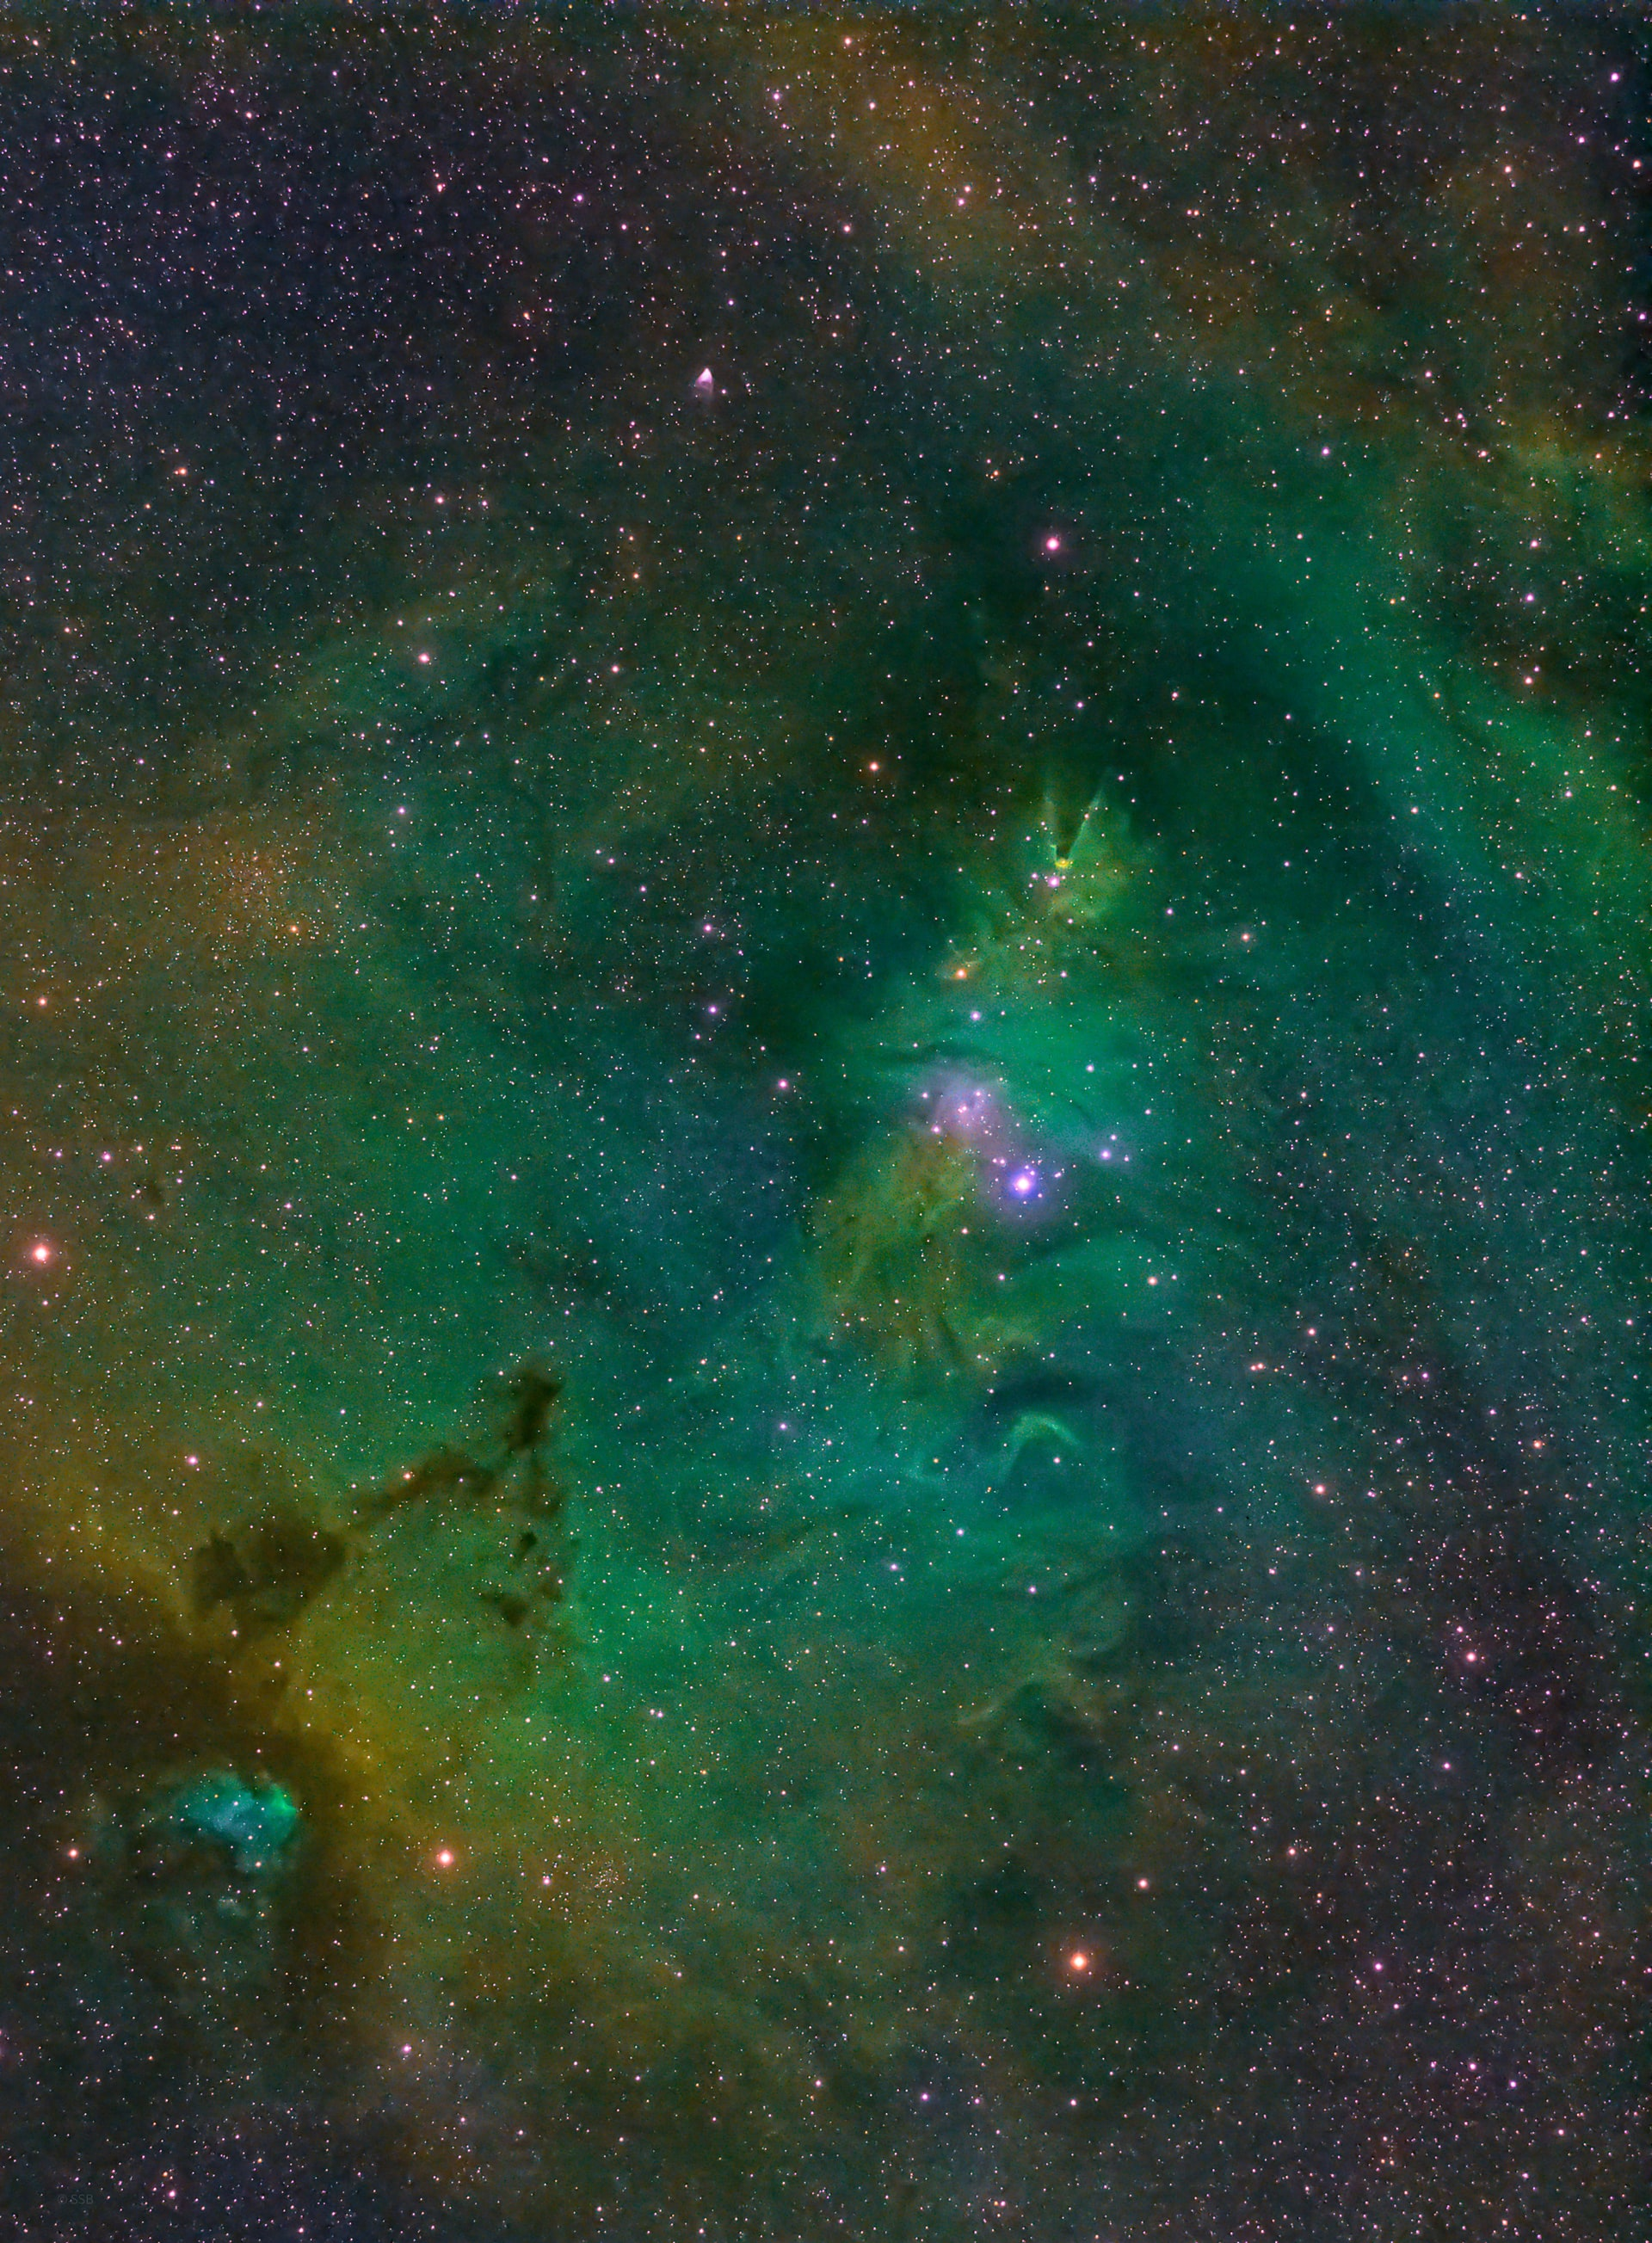
\includegraphics[width=\paperwidth]{./img/aldebaran.jpg}}
\begin{frame}
\huge{\textcolor{white}{\textbf{0x5: Cross-Site-Scripting (XSS)}}}
\end{frame}
}

\section{0x6: SQL Injection}
{
\usebackgroundtemplate{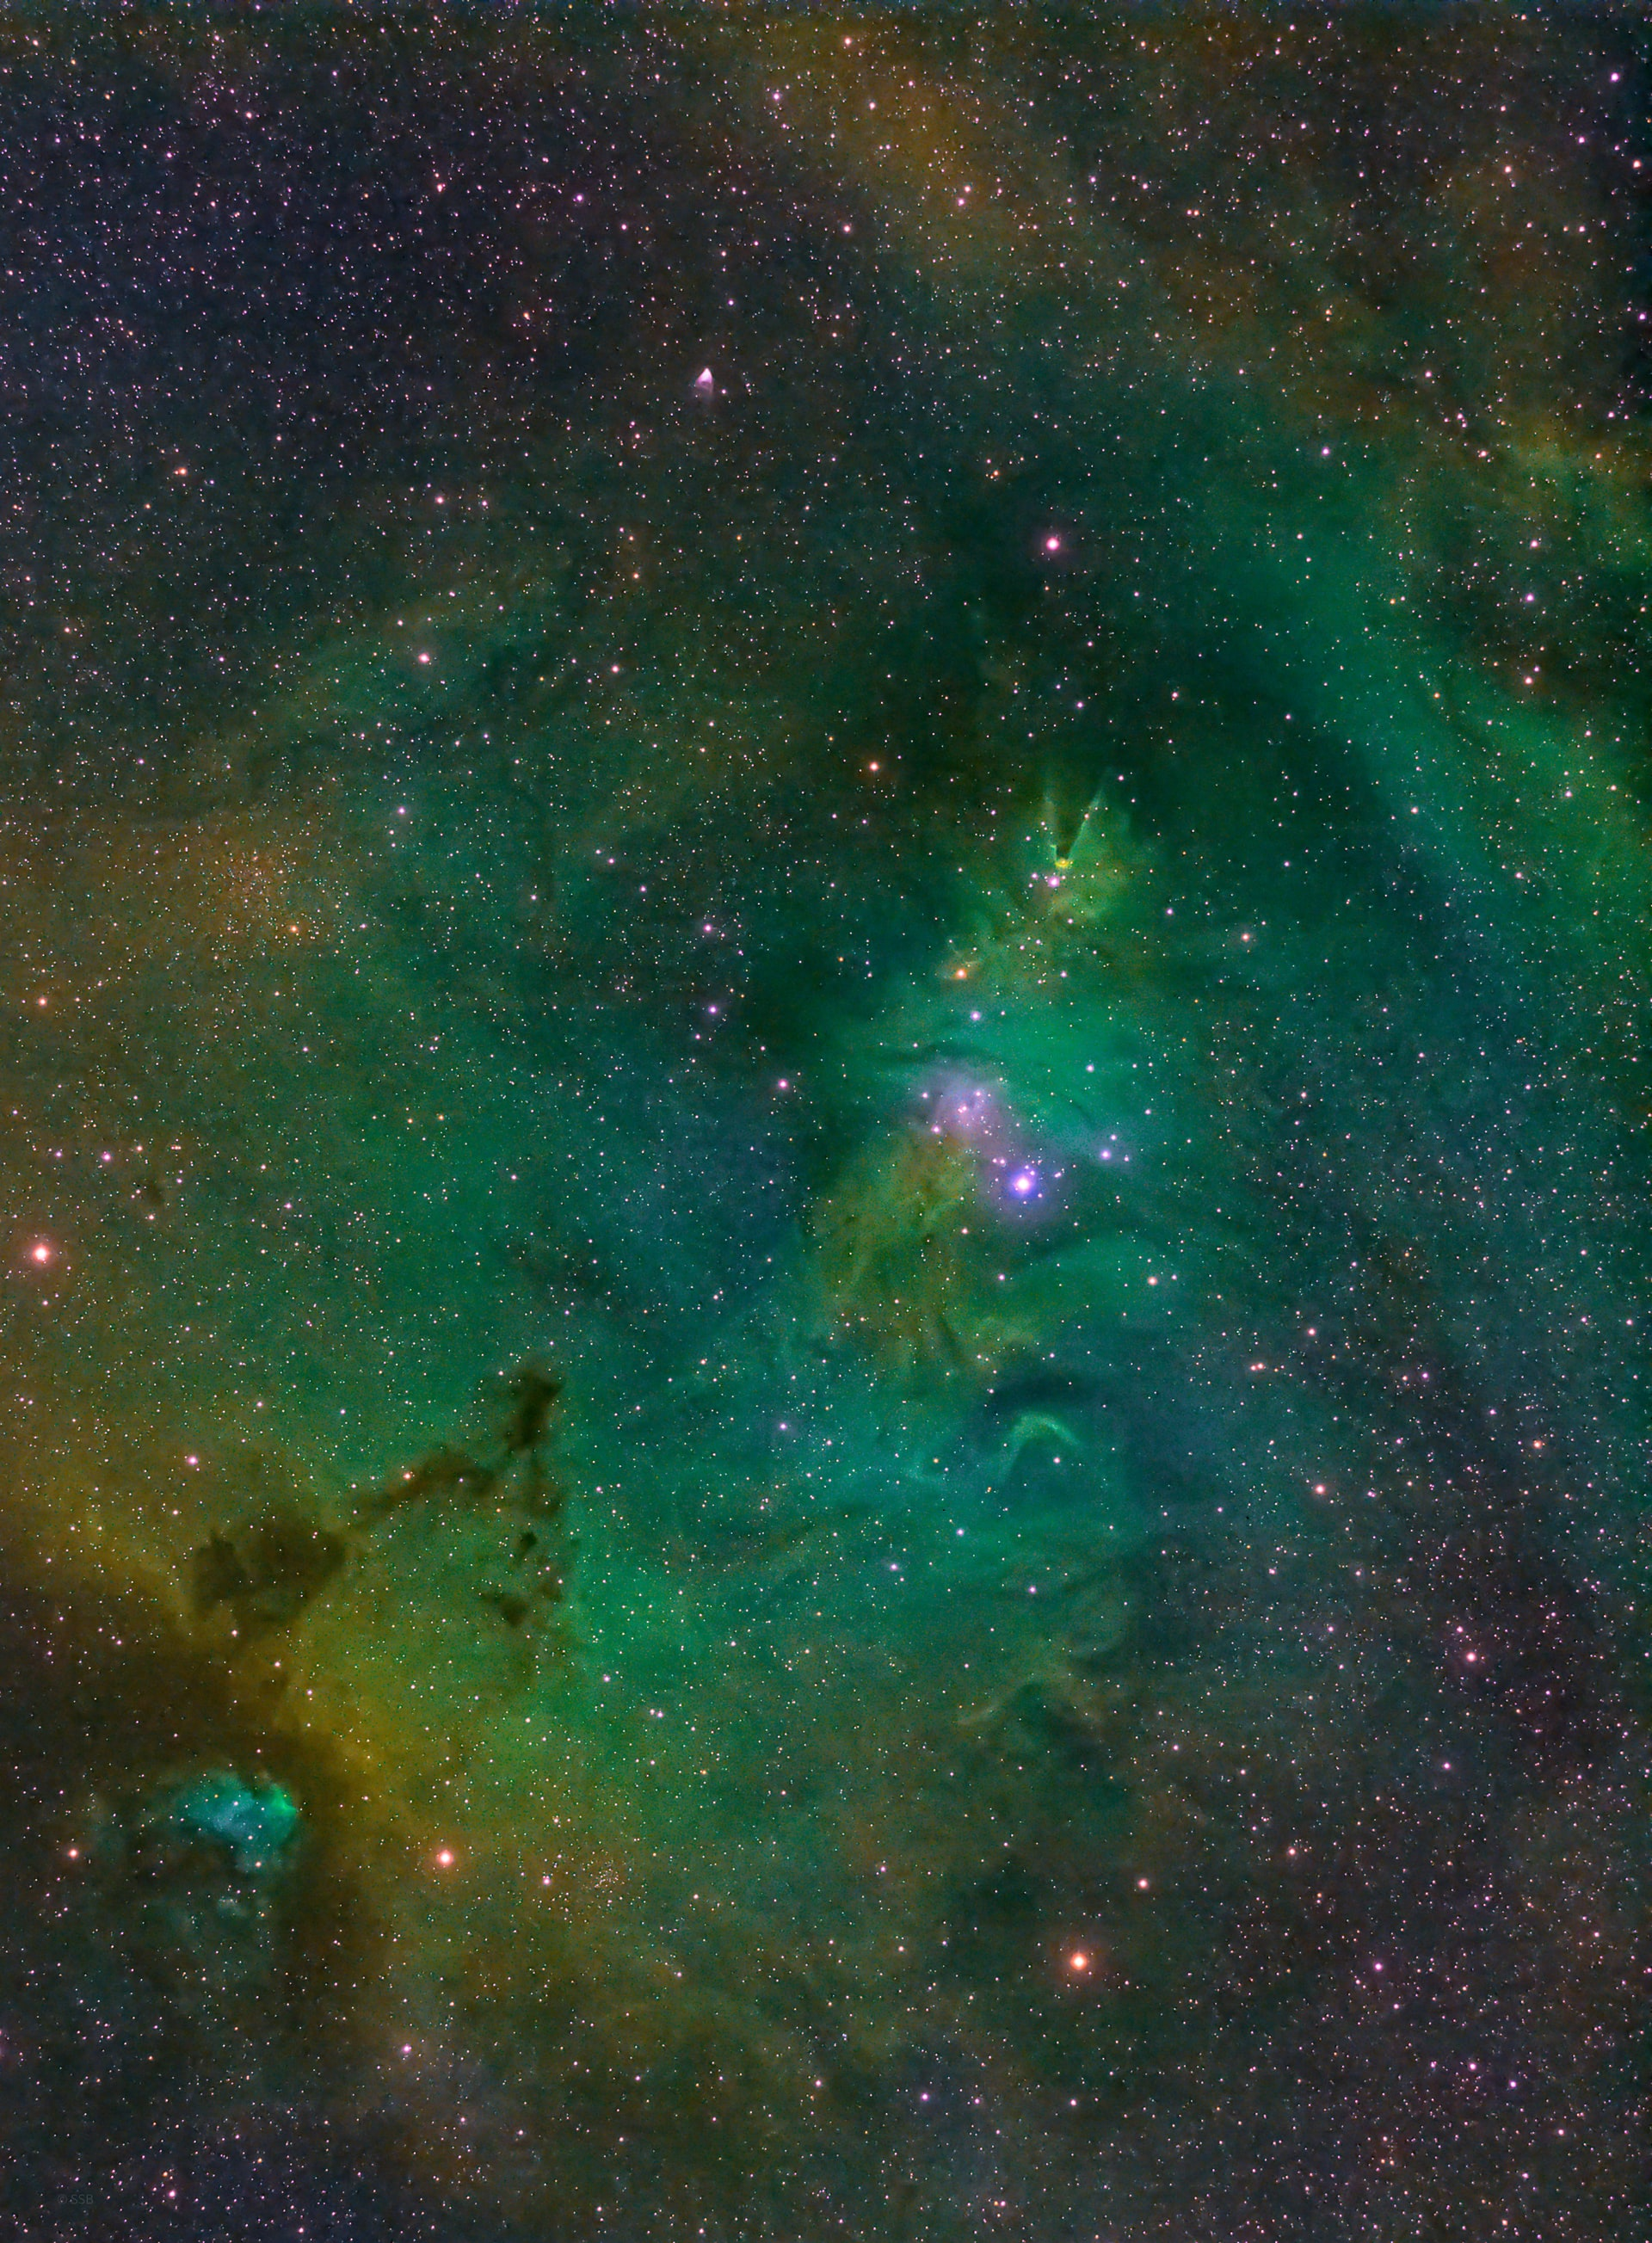
\includegraphics[width=\paperwidth]{./img/aldebaran.jpg}}
\begin{frame}
\huge{\textcolor{white}{\textbf{0x6: SQL Injection}}}
\end{frame}
}

\section{0x7: Other Injection-Based Vulnerabilities}
{
\usebackgroundtemplate{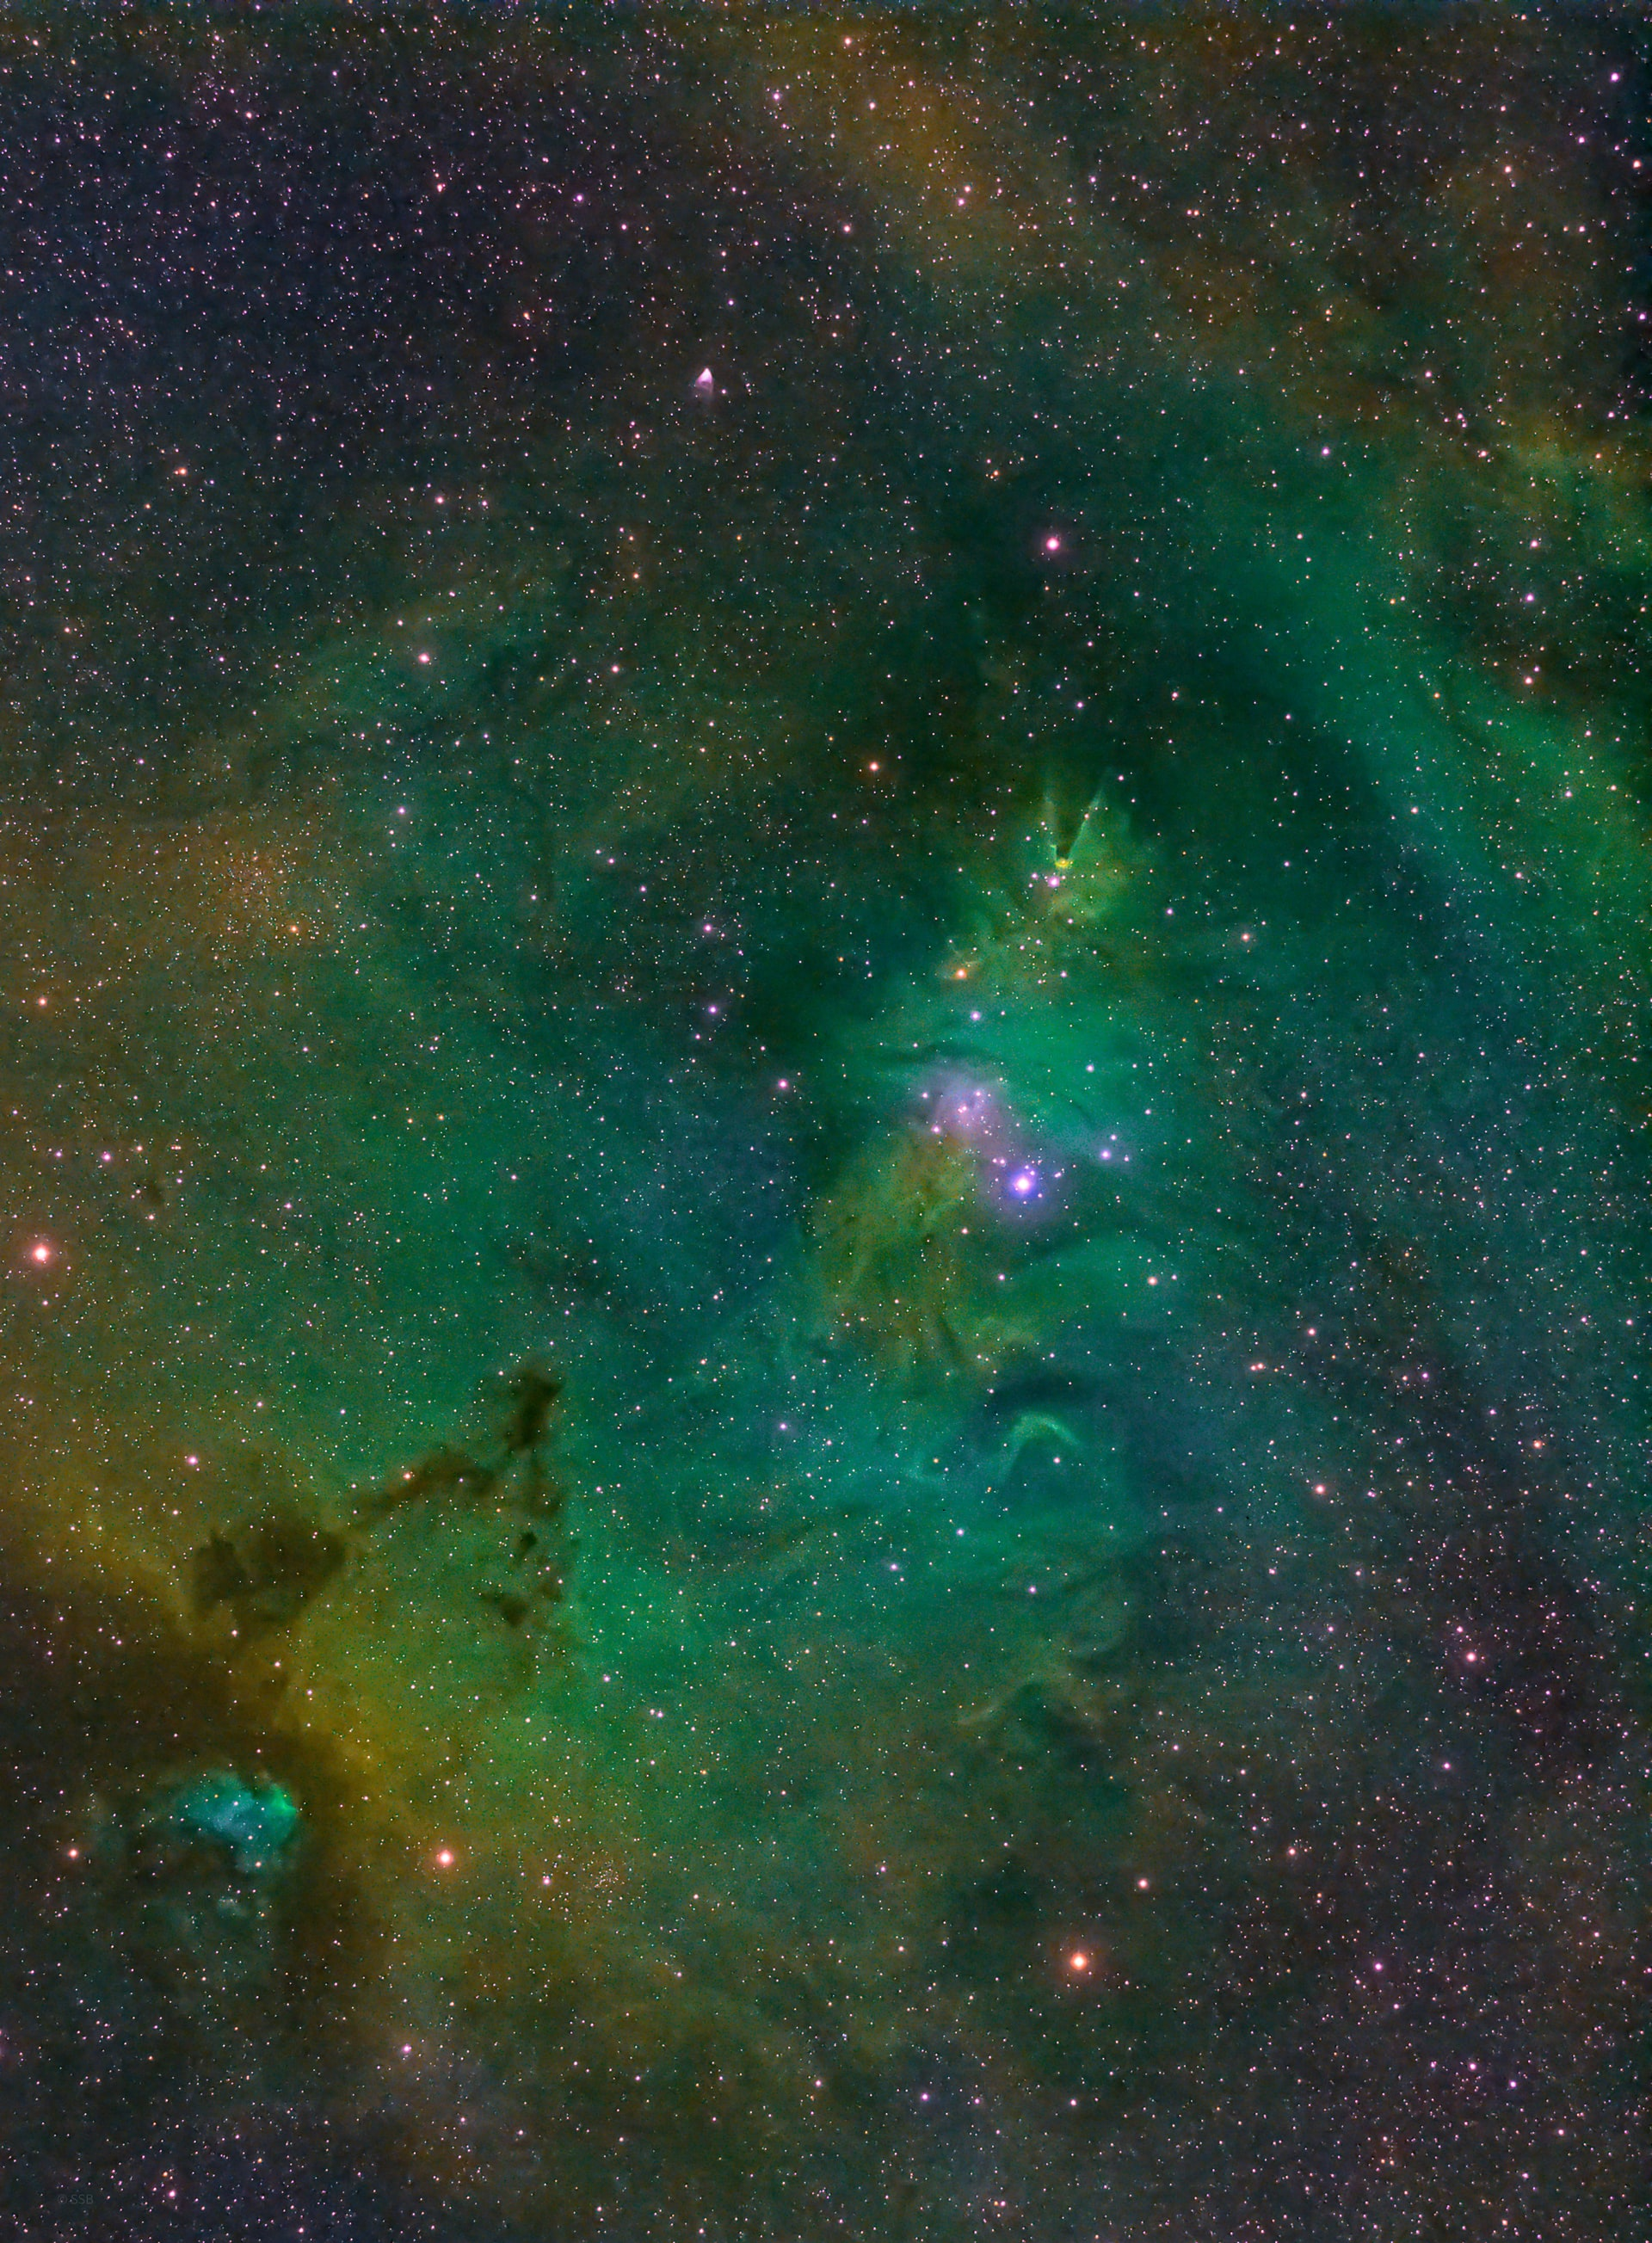
\includegraphics[width=\paperwidth]{./img/aldebaran.jpg}}
\begin{frame}
\huge{\textcolor{white}{\textbf{0x7: Other Injection-Based Vulnerabilities}}}
\end{frame}
}

\section{0x8: Attacks on File Operations}
{
\usebackgroundtemplate{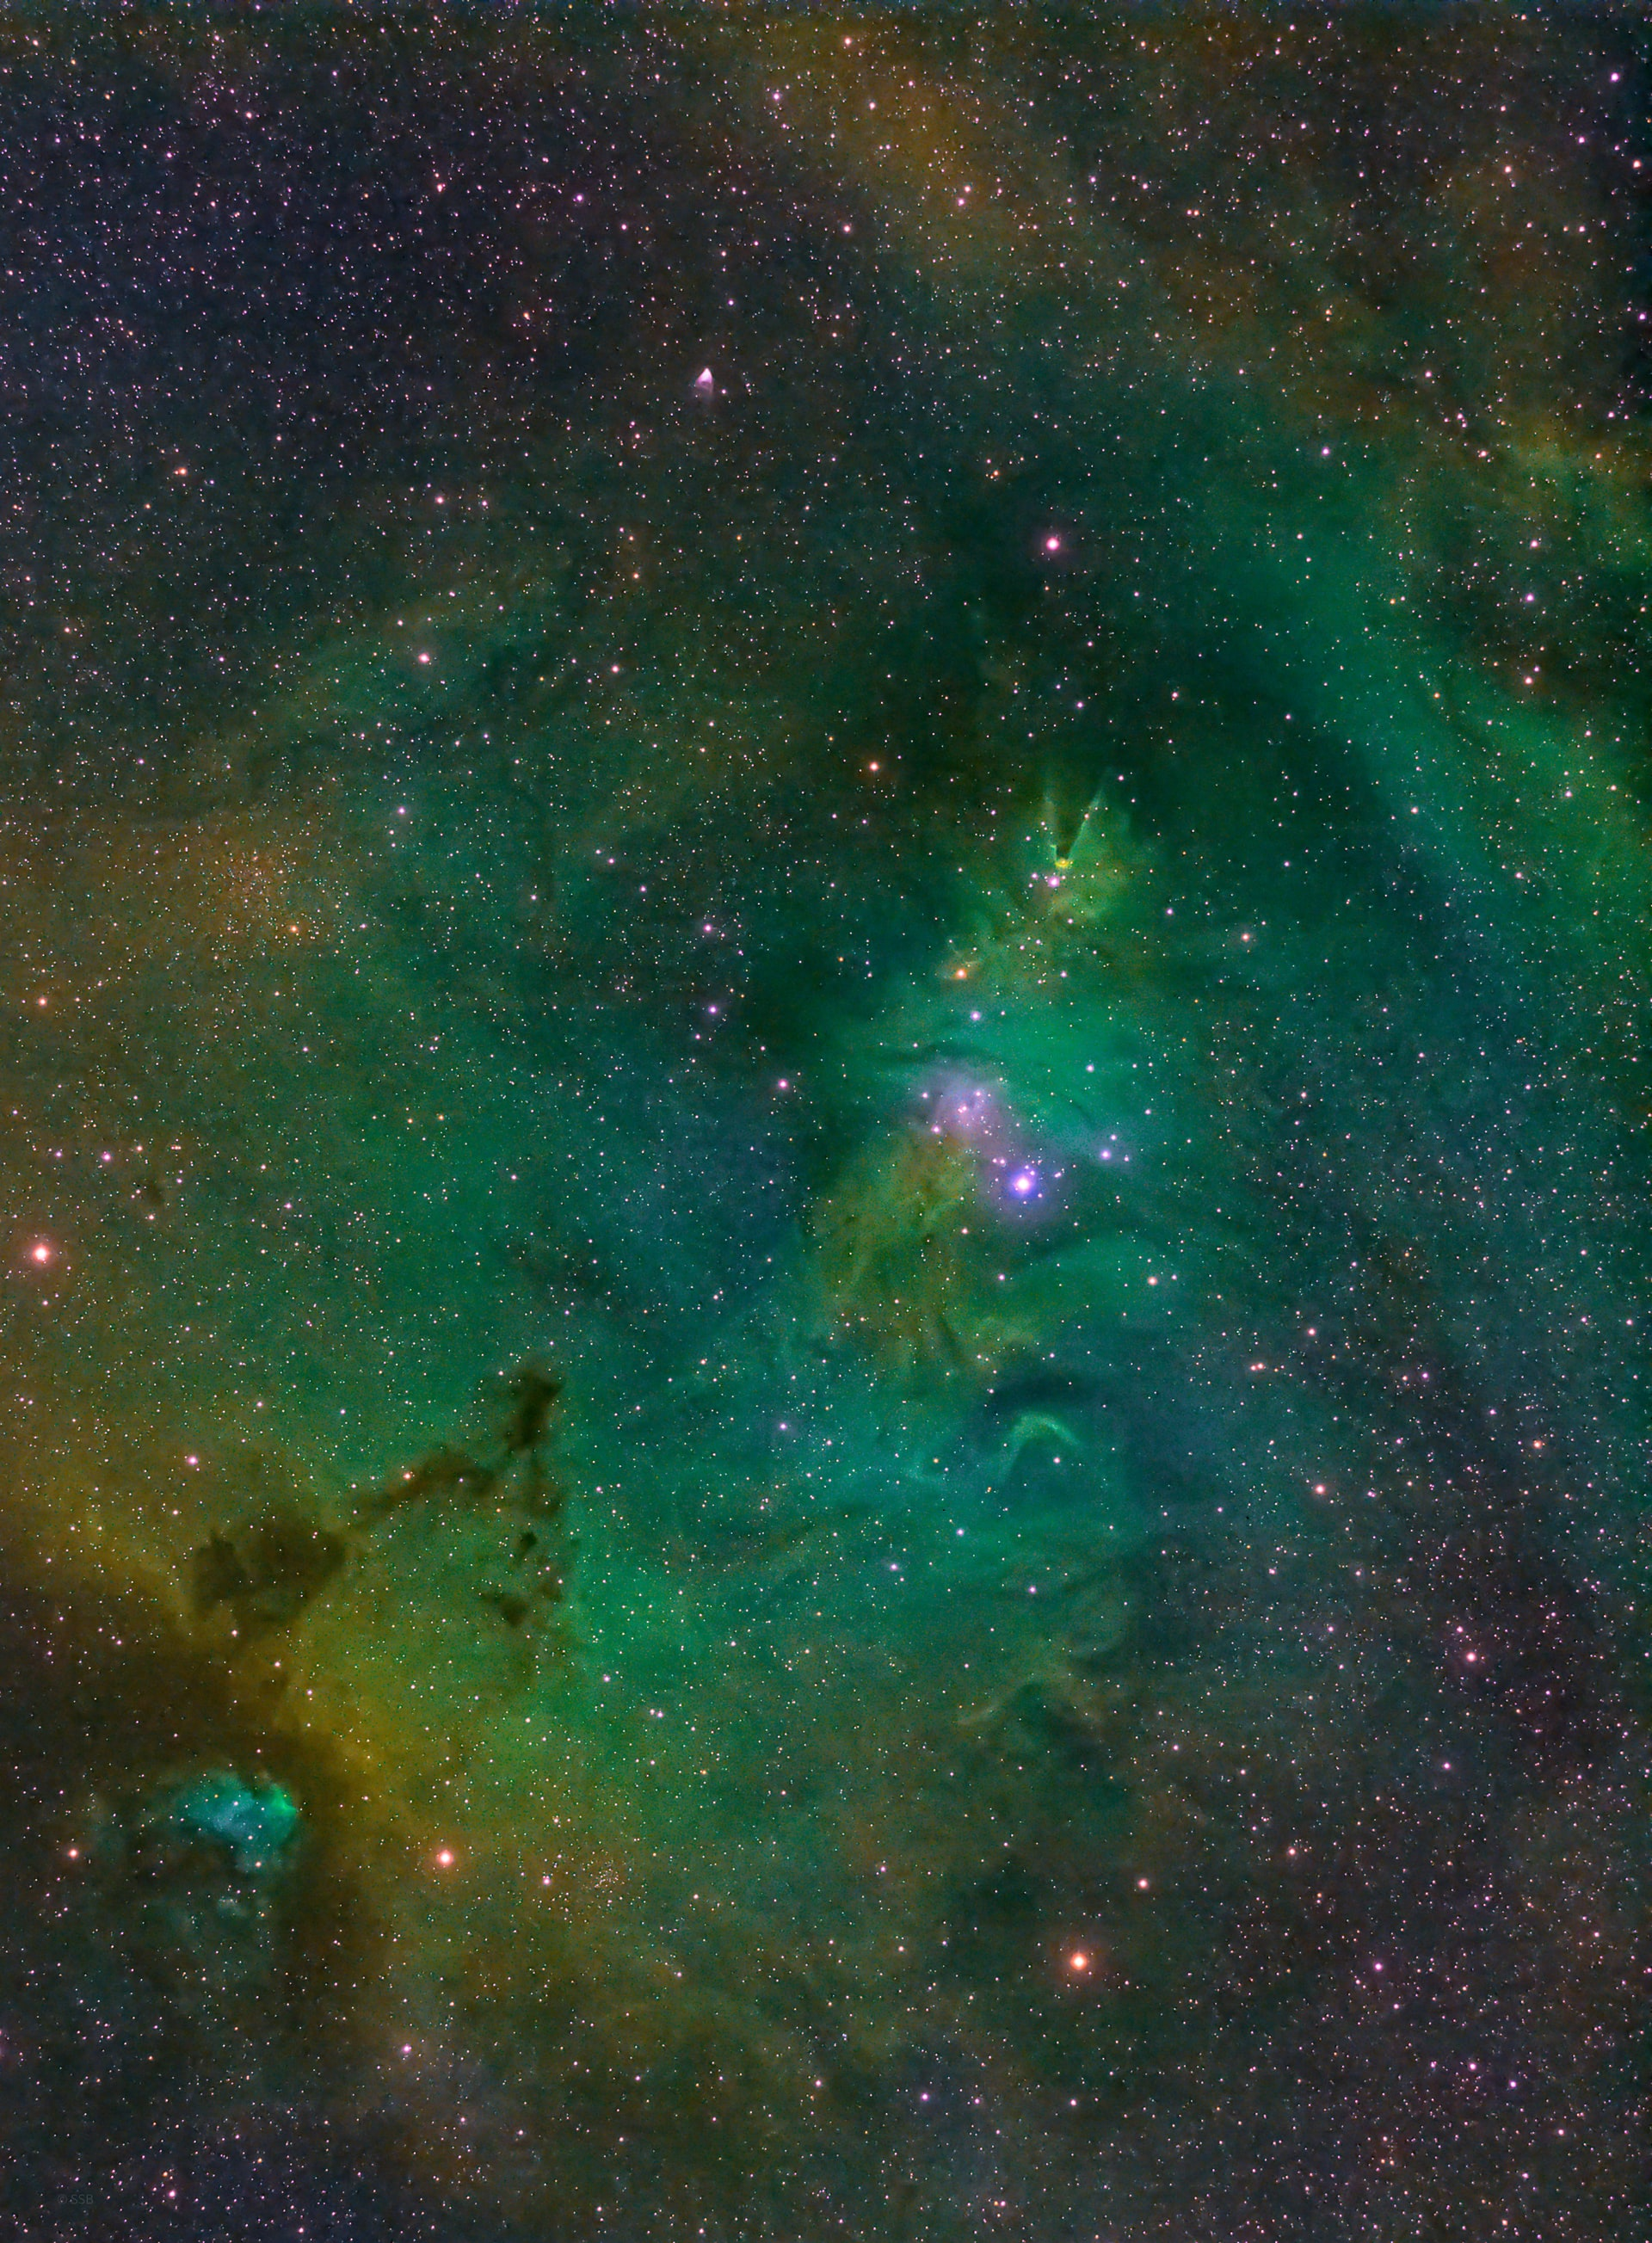
\includegraphics[width=\paperwidth]{./img/aldebaran.jpg}}
\begin{frame}
\huge{\textcolor{white}{\textbf{0x8: Attacks on File Operations}}}
\end{frame}
}

\section{0x9: Buffer Overflows, Format Strings and Integer Bugs}
{
\usebackgroundtemplate{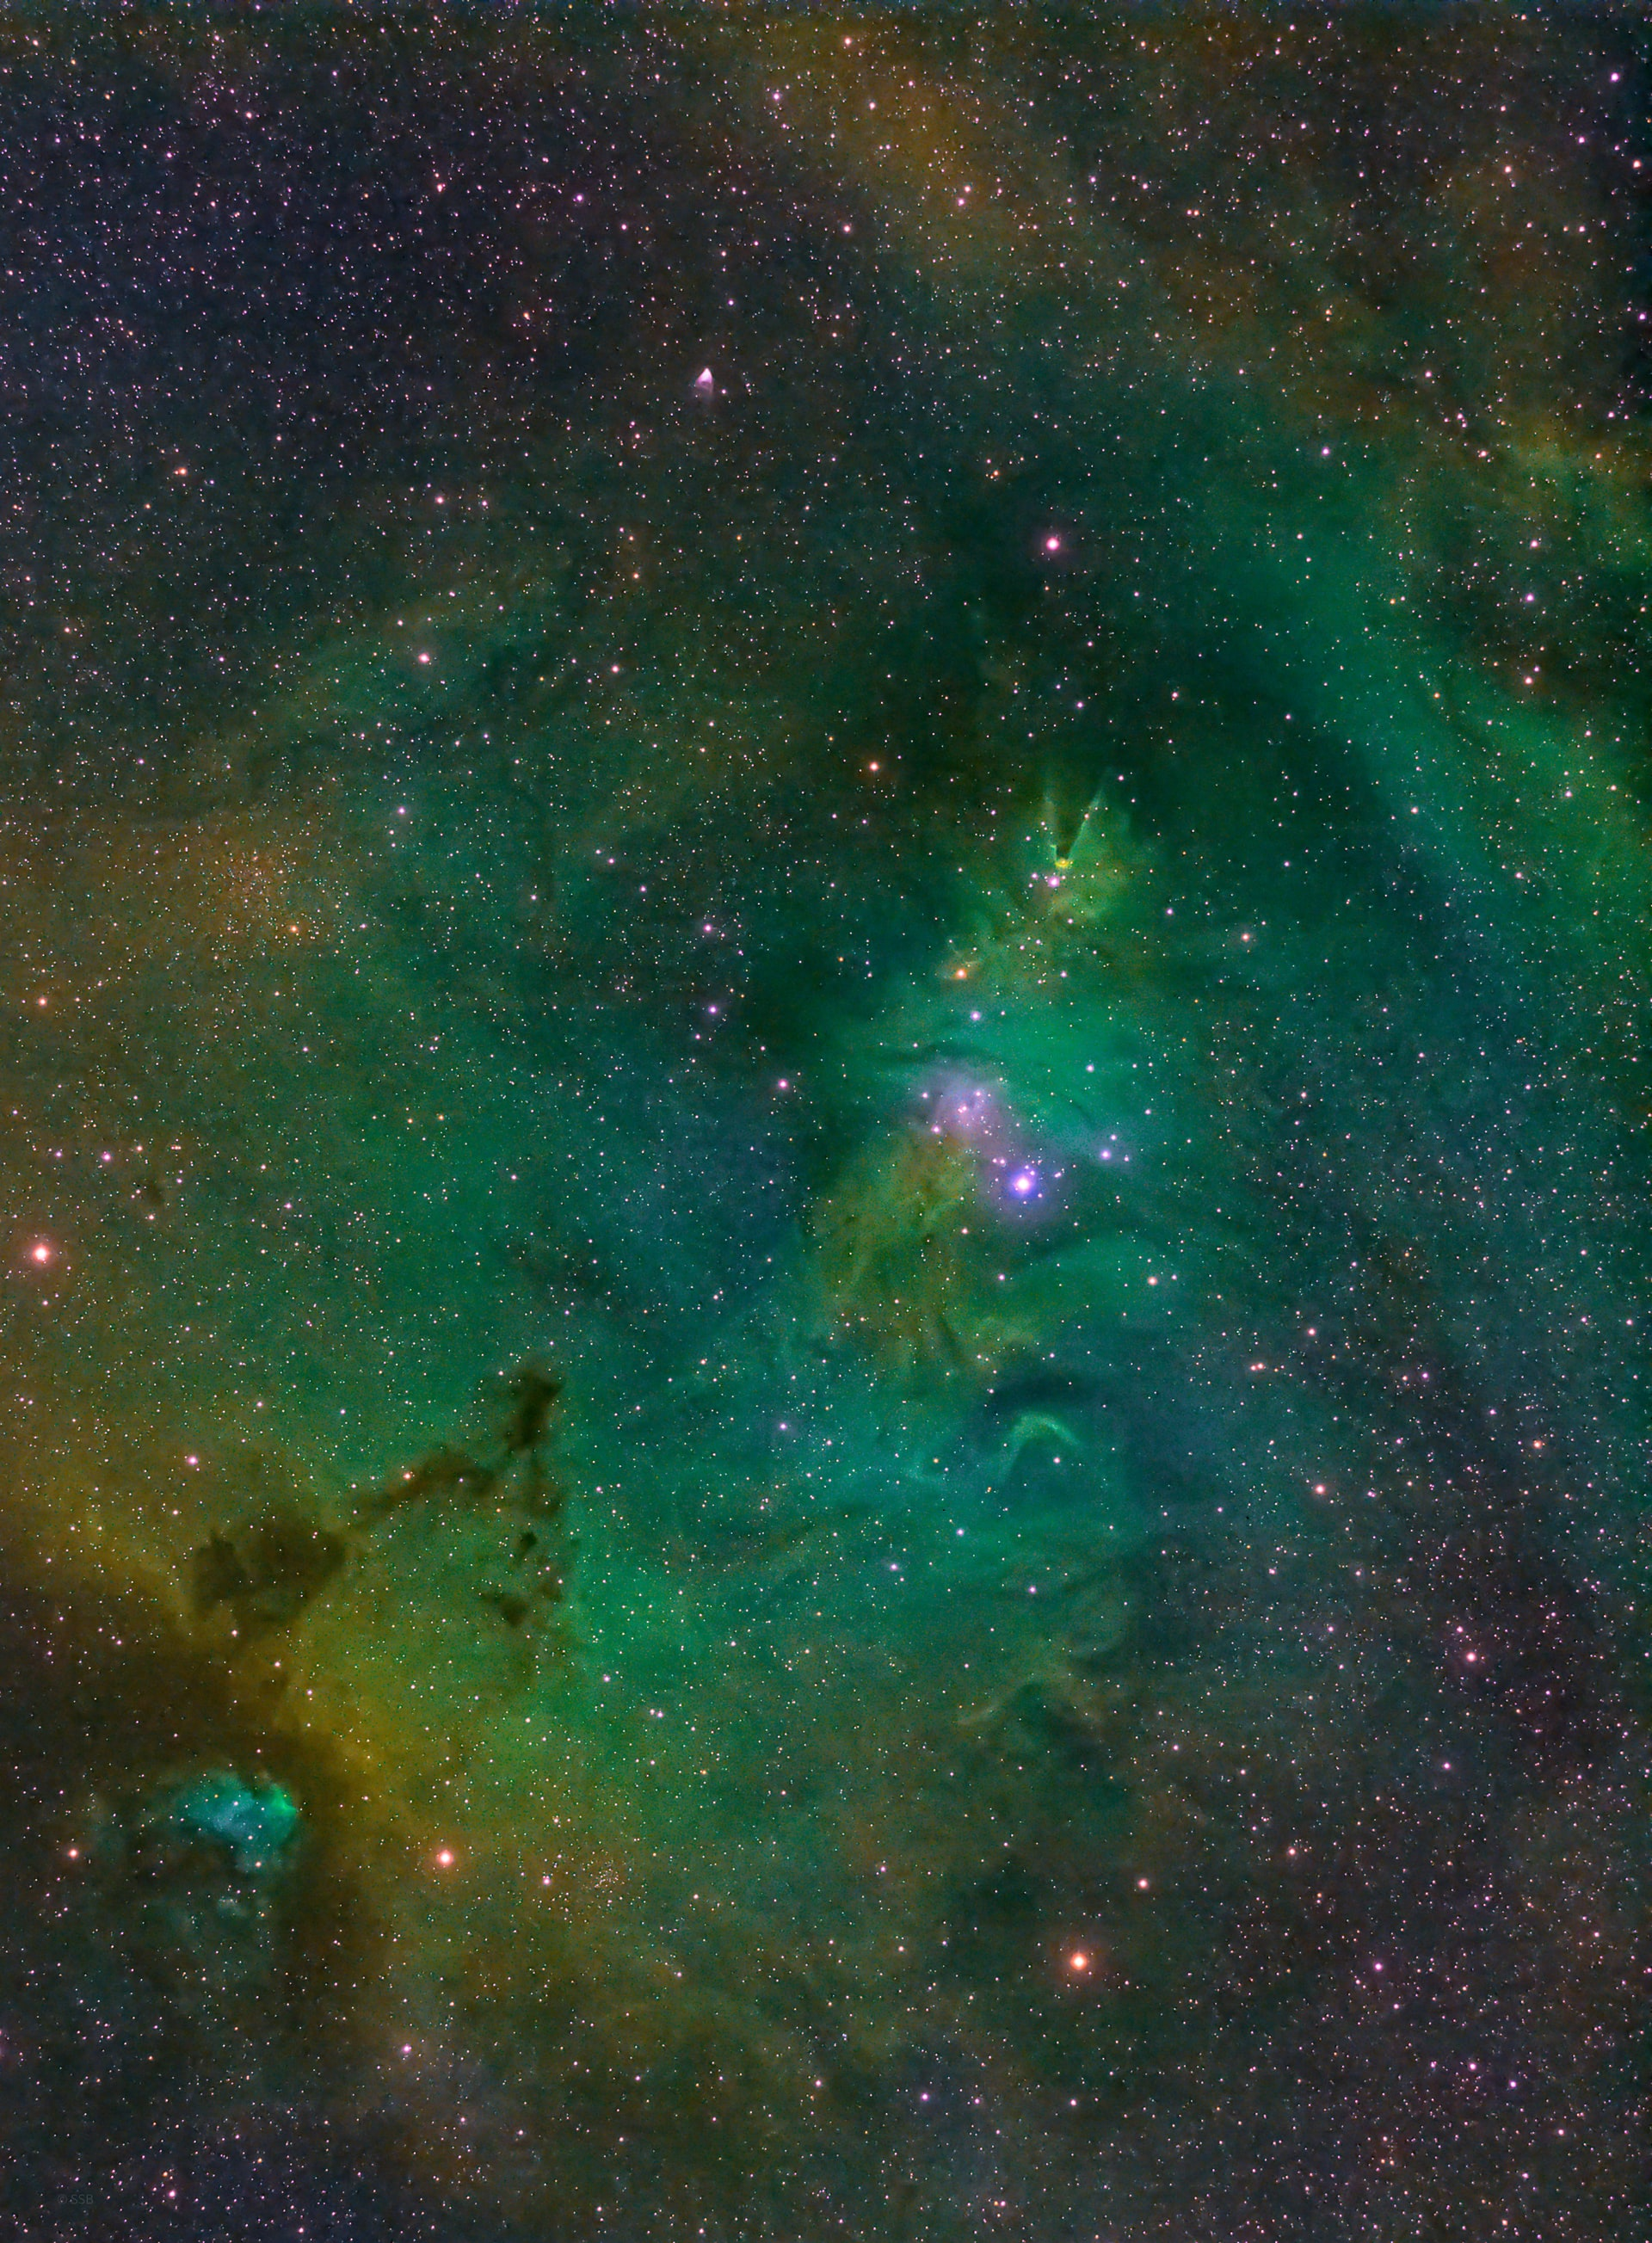
\includegraphics[width=\paperwidth]{./img/aldebaran.jpg}}
\begin{frame}
\huge{\textcolor{white}{\textbf{0x9: Buffer Overflows, Format Strings and Integer Bugs}}}
\end{frame}
}

\section{0xA: Architectural Attacks}
{
\usebackgroundtemplate{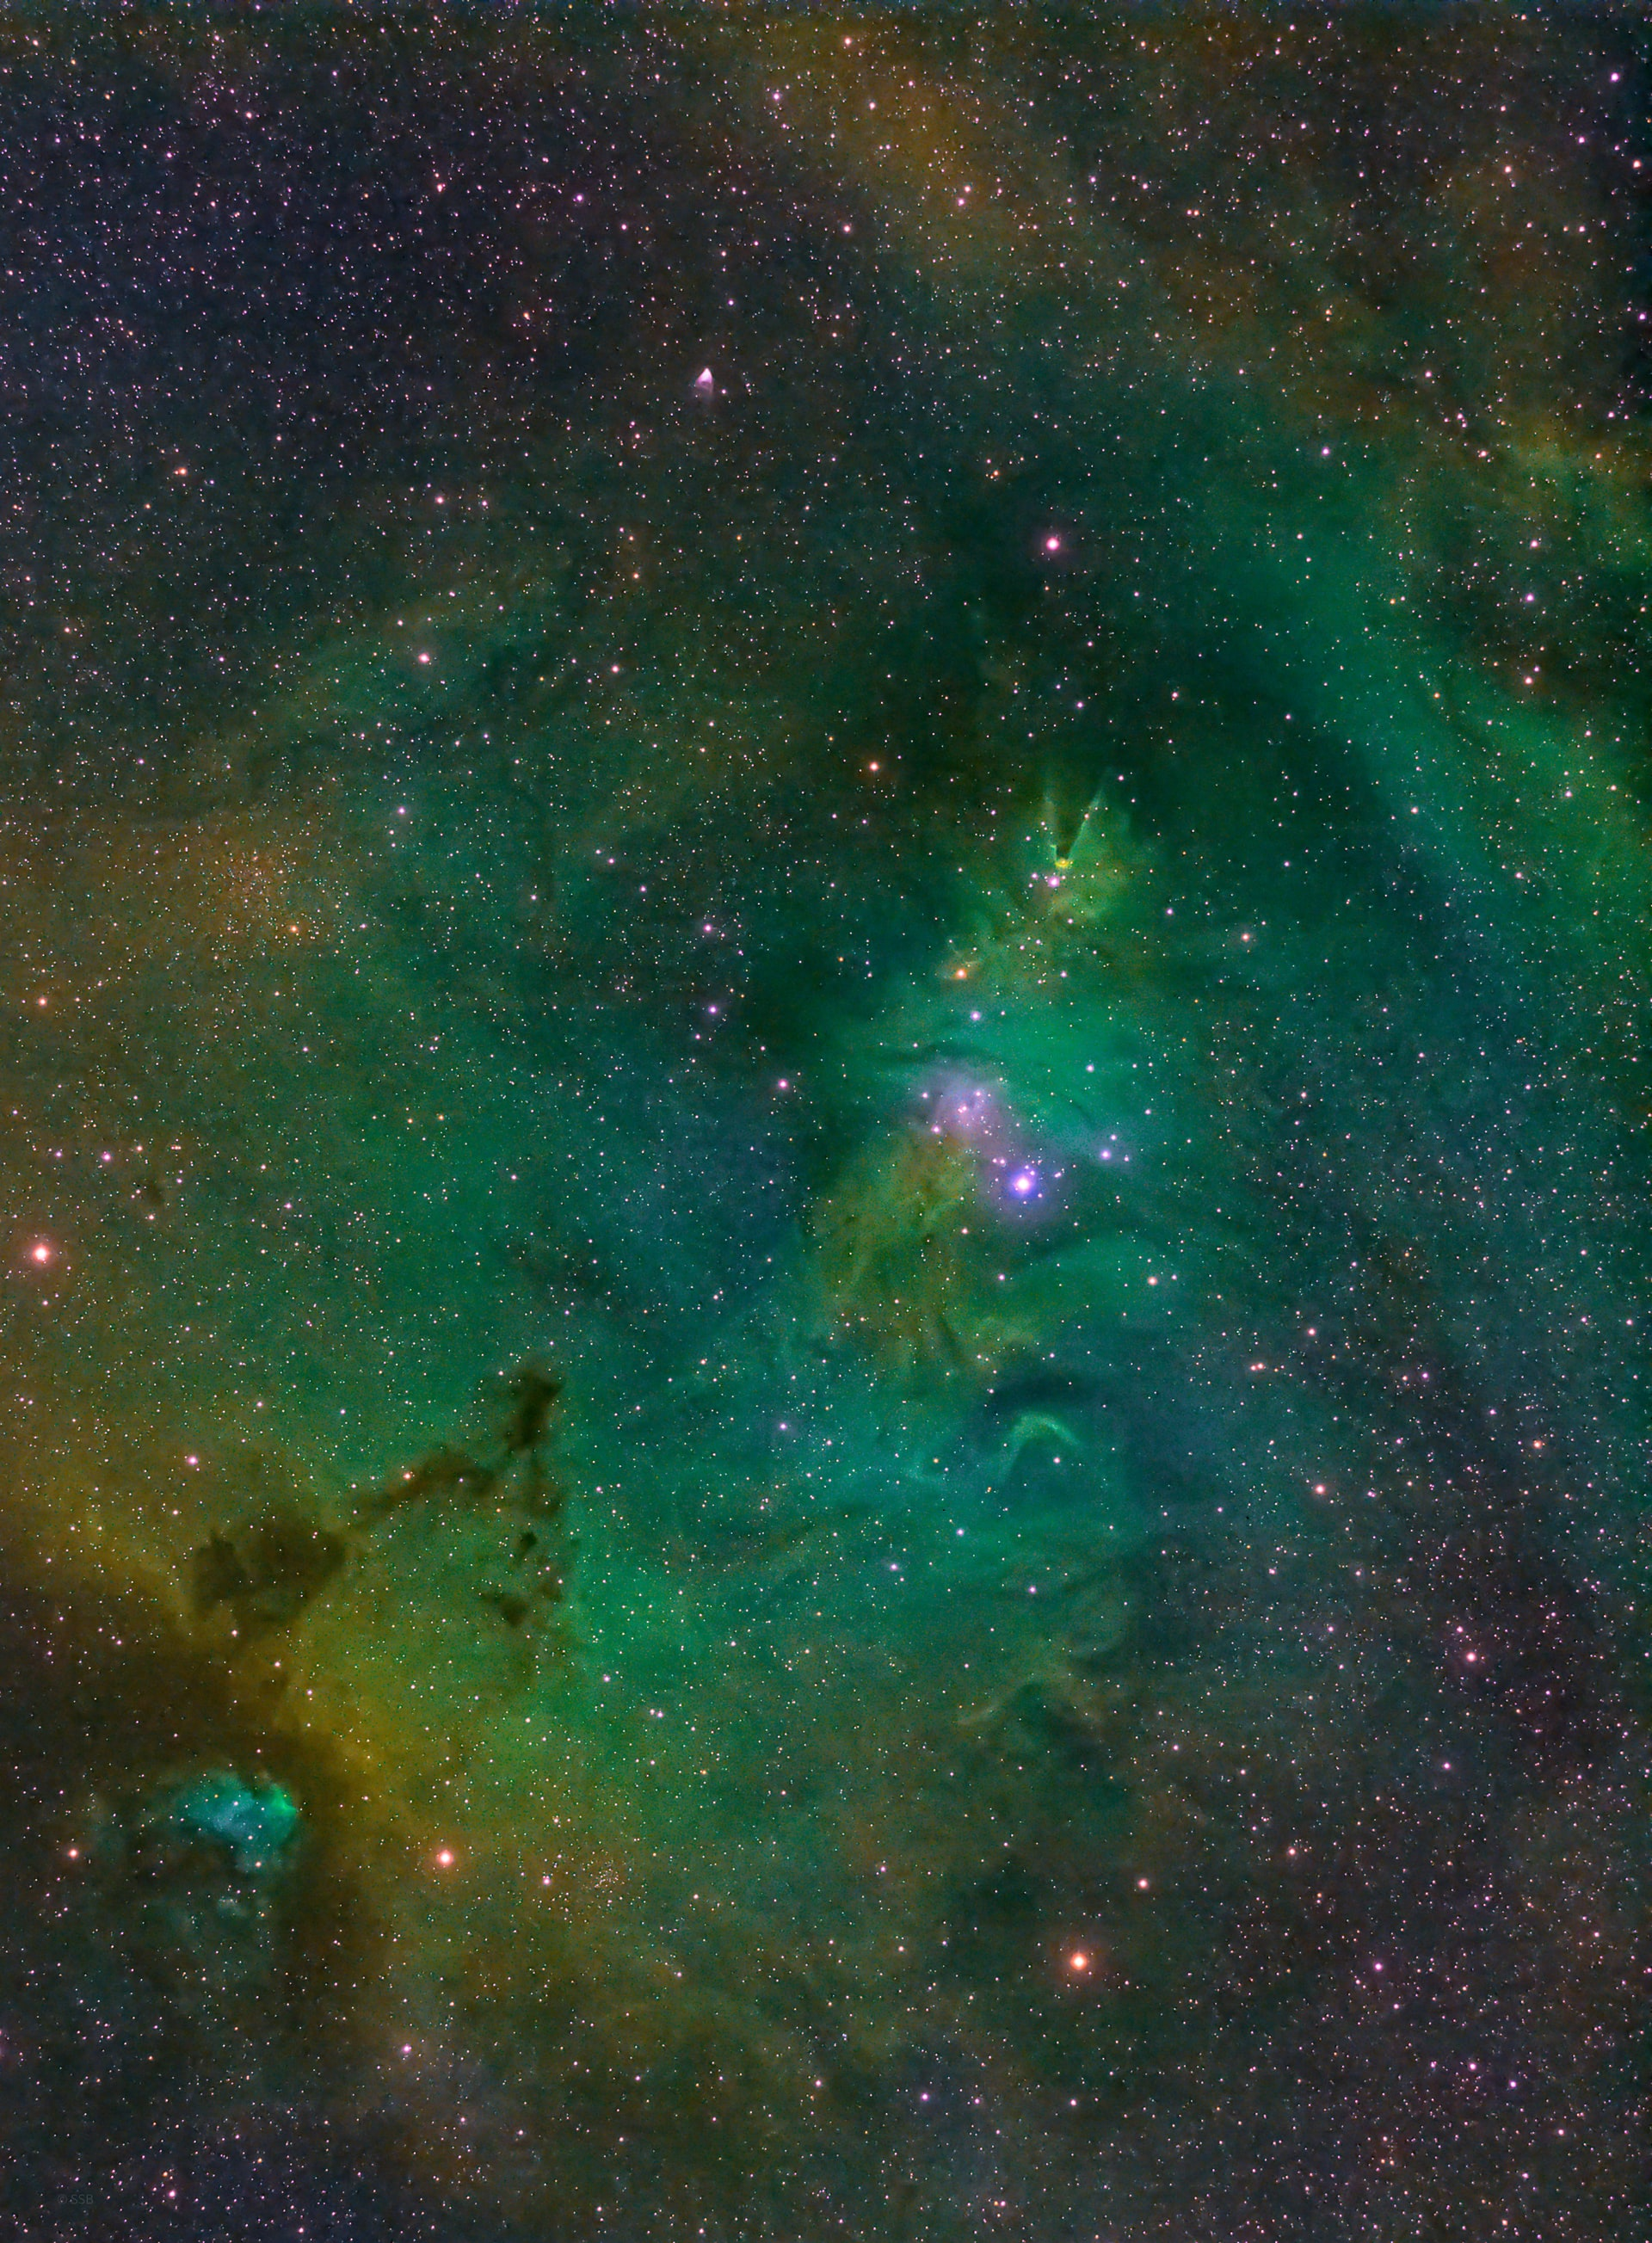
\includegraphics[width=\paperwidth]{./img/aldebaran.jpg}}
\begin{frame}
\huge{\textcolor{white}{\textbf{0xA: Architectural Attacks}}}
\end{frame}
}

\section{0xB: Attacks on the Web Server}
{
\usebackgroundtemplate{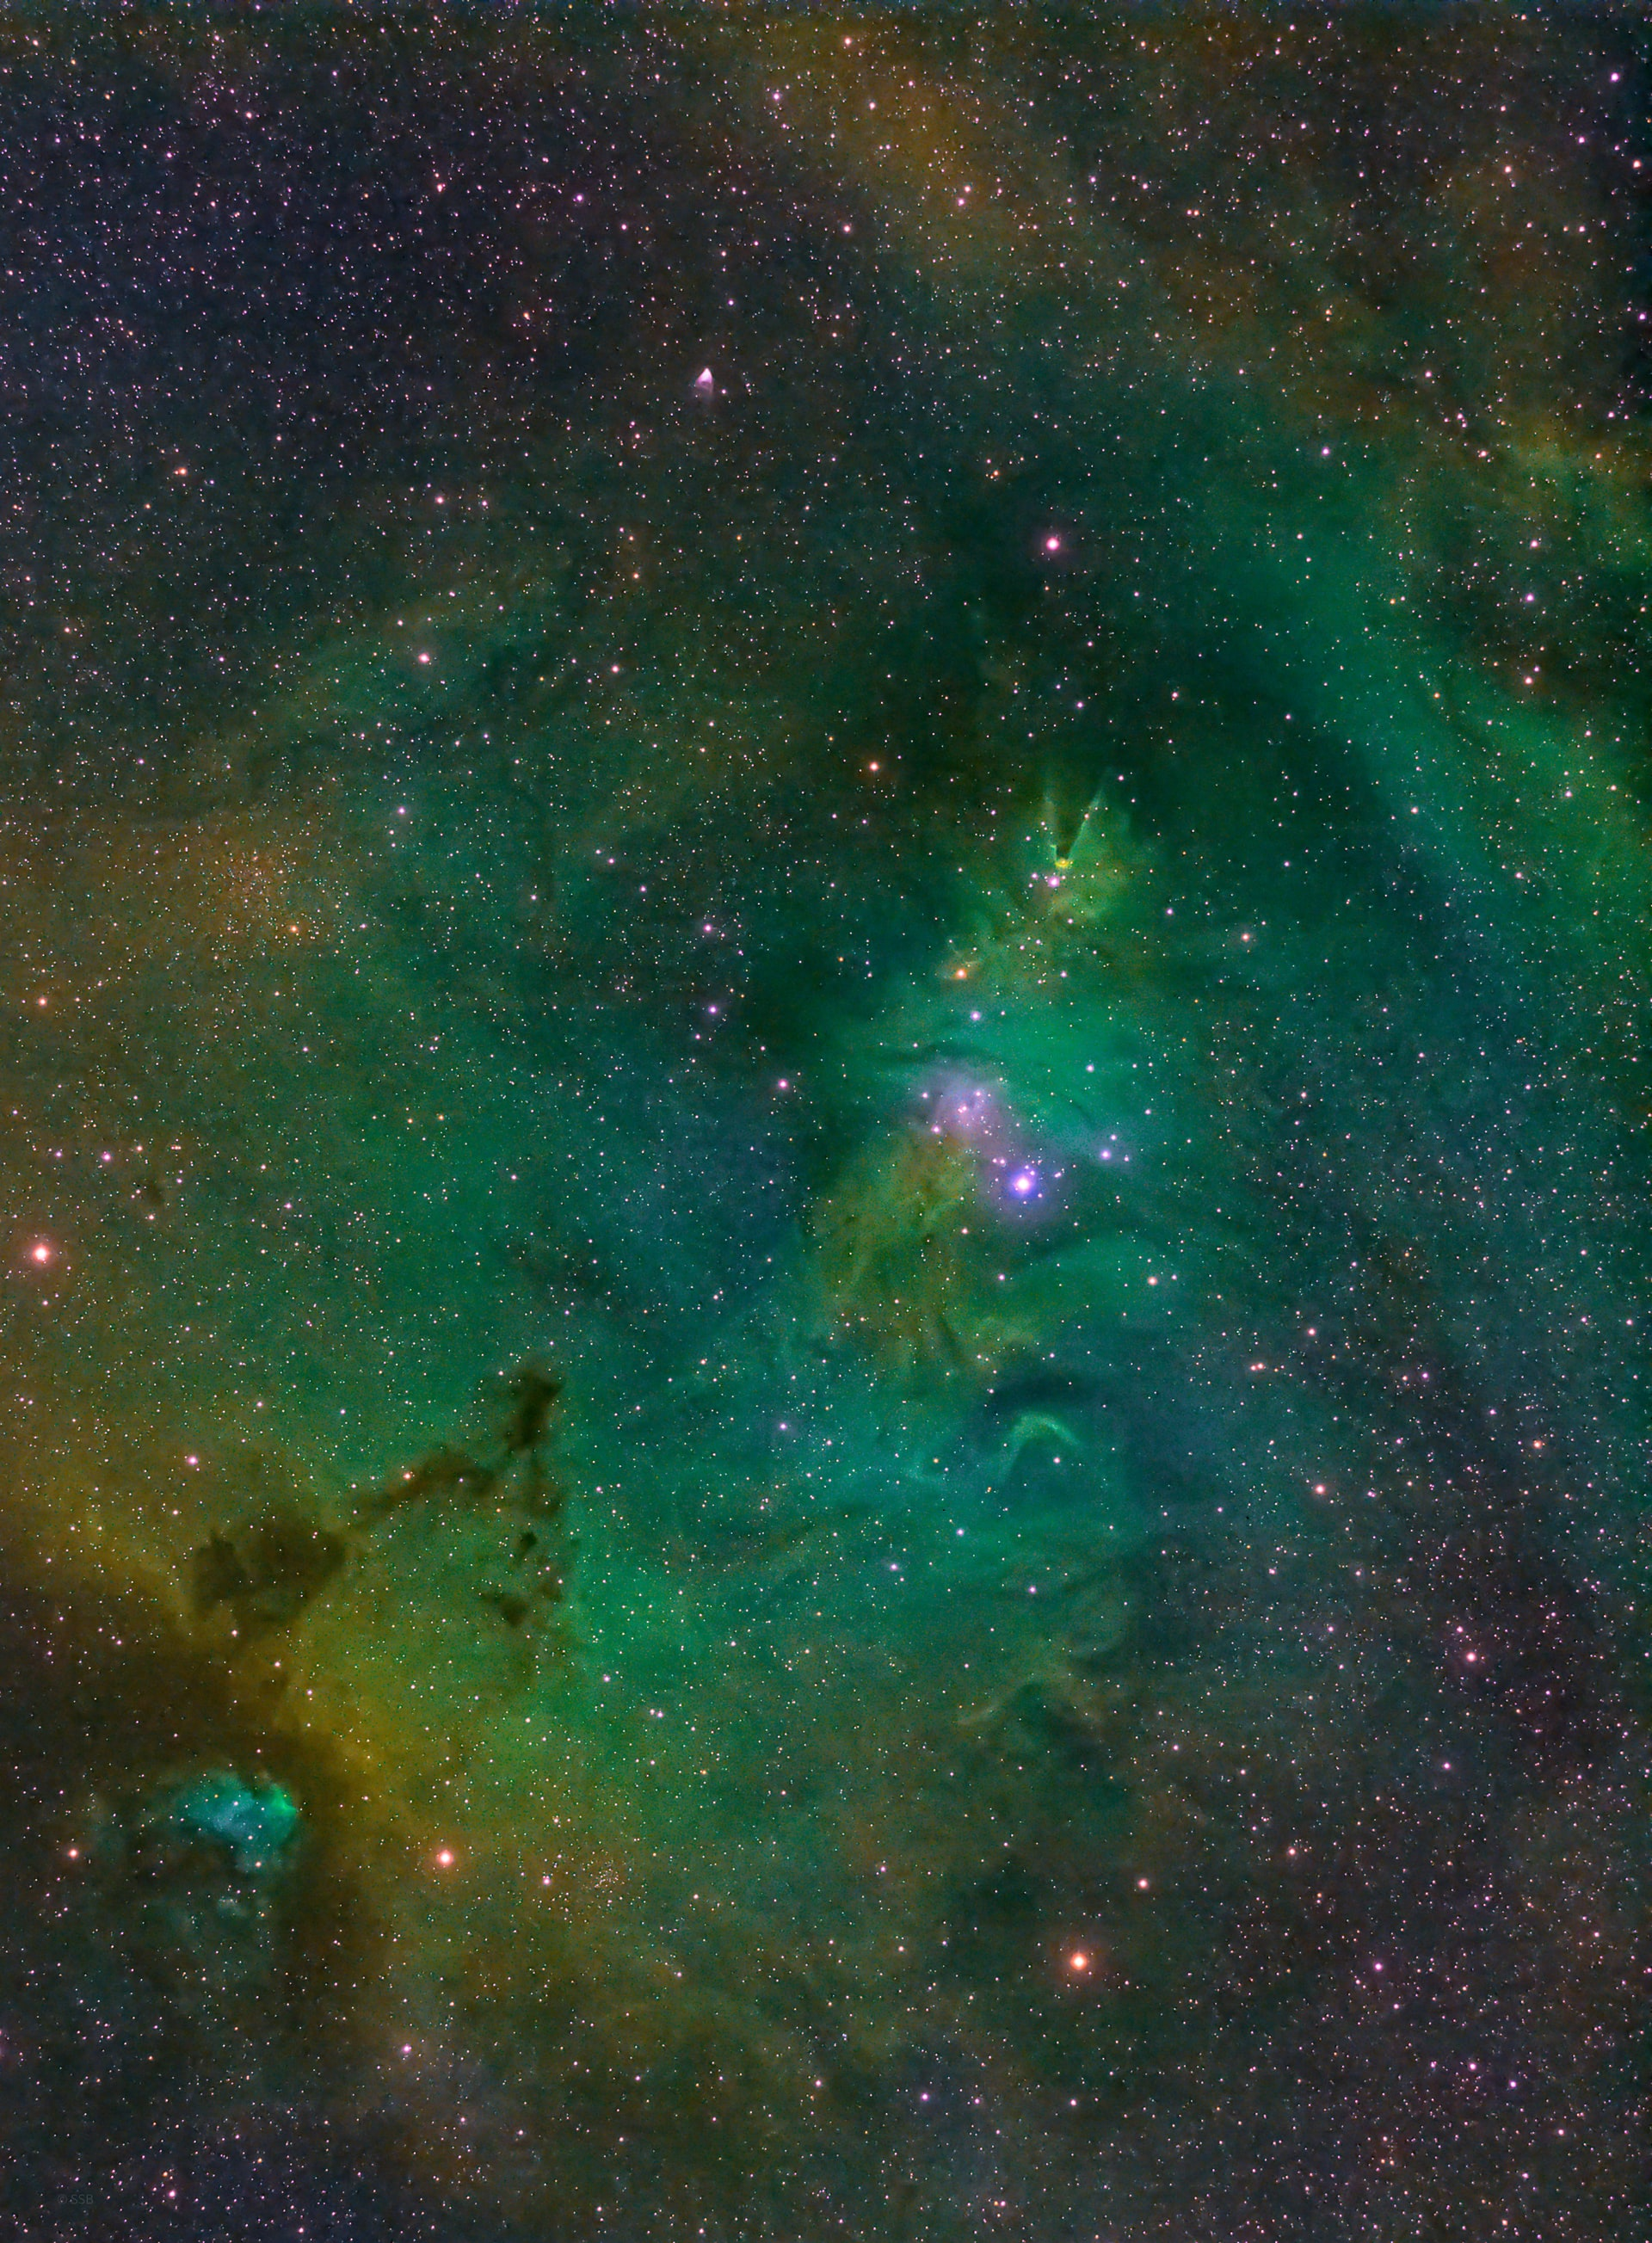
\includegraphics[width=\paperwidth]{./img/aldebaran.jpg}}
\begin{frame}
\huge{\textcolor{white}{\textbf{0xB: Attacks on the Web Server}}}
\end{frame}
}


{
\usebackgroundtemplate{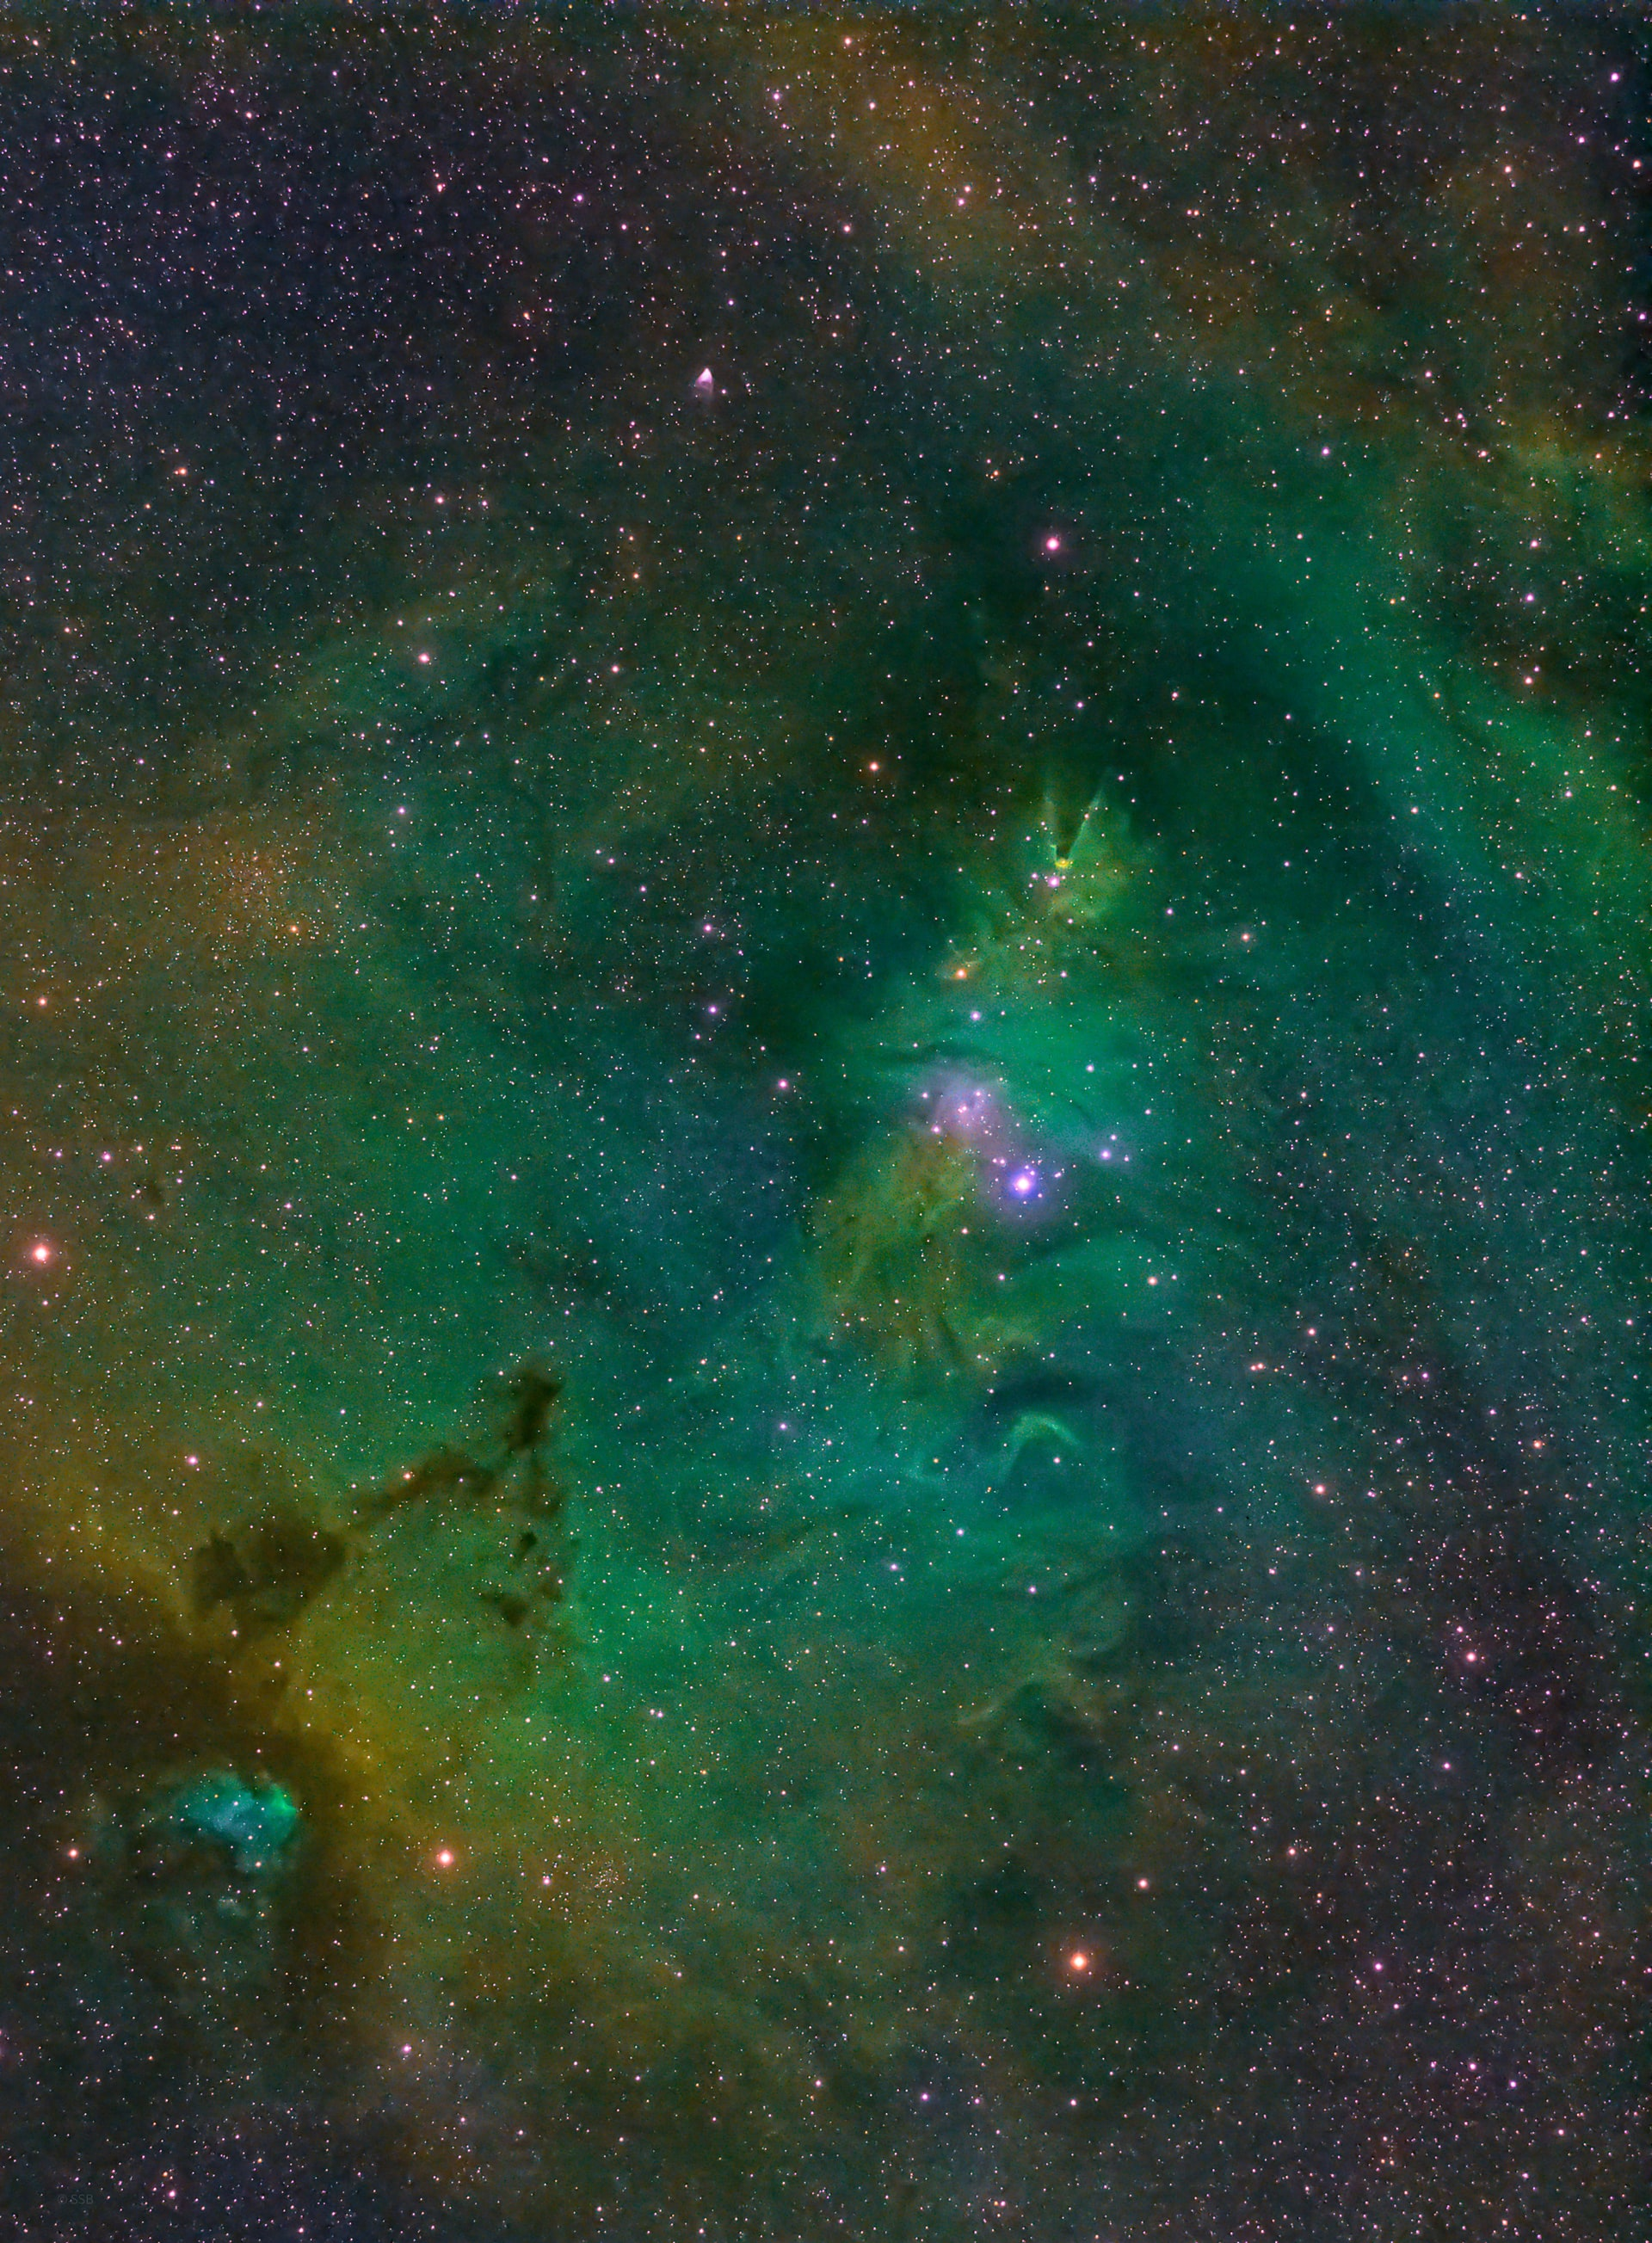
\includegraphics[width=\paperwidth]{./img/aldebaran.jpg}}
\begin{frame}
\huge{\textcolor{white}{\textbf{0xC: Misc}}}
\end{frame}
}

\begin{frame}
    \frametitle{More Things to Consider}
    One \pause
    Two \pause
    Three
\end{frame}

\begin{frame}
    \frametitle{Bibliography}

\end{frame}

\bibliographystyle{plain}
\bibliography{ref/bibliography}

\end{document}